\documentclass{article}
\usepackage[utf8]{inputenc}
\usepackage[T1]{fontenc}
\usepackage{mathtools}
\usepackage{amssymb}
\usepackage{amsmath}
\usepackage{amsthm}
%\usepackage{csquotes}
\usepackage{amsfonts}
\usepackage[ngerman]{babel}
\usepackage[linesnumbered,ruled]{algorithm2e}
\usepackage[hidelinks]{hyperref}
\usepackage{graphicx}
\usepackage{ulem}
\usepackage{icomma}
\usepackage{bbm}
\usepackage{eufrak}
\usepackage{upgreek}
\usepackage{bm}
\usepackage{fix-cm}

\usepackage{mathtools}

\usepackage{tikz}
\usetikzlibrary{datavisualization}
\usetikzlibrary{datavisualization.formats.functions}

%\usepackage{geometry}
%\geometry{left=47.2mm, right=47.2mm, top=44mm}

\relpenalty=10000
\binoppenalty=10000

\usepackage{stackengine,scalerel,graphicx,amssymb,amsmath,wasysym}

%New sum symbols
\DeclareMathOperator*{\Sigmacirc}{%
  \ThisStyle{\mathop{\ensurestackMath{\stackinset{c}{-0.75\LMpt}{c}{}{%
  \rotatebox[origin=lb]{-90}{$\circ$}}{\SavedStyle\Sigma}}}}}

\DeclareMathOperator*{\sumcirc}{%
  \ThisStyle{\mathop{\ensurestackMath{\stackinset{c}{-1.5\LMpt}{c}{}{%
  \rotatebox[origin=lb]{-90}{$\SavedStyle\scalerel*{\bm\Circle}{%
  i}$}}{\SavedStyle\sum}}}}}

\DeclareMathOperator*{\sumbar}{\overline{\sum}}

\newcommand{\algebra}{\mathbin{
  \mathchoice
    {\mbox{\normalsize\textcircled{\scriptsize A}}}
    {\mbox{\normalsize\textcircled{\scriptsize A}}}
    {\mbox{\scriptsize\textcircled{\tiny A}}}
    {\mbox{\tiny\textcircled{\fontsize{3.5}{3.5}\selectfont A}}}
  }
}

\newcommand{\mink}{\mathbin{
  \mathchoice
    {\mbox{\normalsize\textcircled{\scriptsize M}}}
    {\mbox{\normalsize\textcircled{\scriptsize M}}}
    {\mbox{\scriptsize\textcircled{\tiny M}}}
    {\mbox{\tiny\textcircled{\fontsize{3.5}{3.5}\selectfont M}}}
  }
}

\begin{document}

\SetArgSty{textnormal}

\newtheorem{theorem}{Satz}
\numberwithin{theorem}{section}

\newtheorem{lemma}{Lemma}
\numberwithin{lemma}{section}

\newtheorem{corollary}{Korollar}
\numberwithin{corollary}{section}

\theoremstyle{remark}
\newtheorem{example}{Beispiel}
\numberwithin{example}{section}

\theoremstyle{definition}
\newtheorem{definition}{Definition}
\numberwithin{definition}{section}

\theoremstyle{remark}
\newtheorem{remark}{Anmerkung}
\numberwithin{remark}{section}

\begin{titlepage}
\title{Methoden algewandter Algebra 1/2}
\date{\today}
\author{Alex Ivliev}
\maketitle
\end{titlepage}

\tableofcontents 
\newpage

\section{allgemeine Definitionen}
\begin{definition}
  Die Menge der natürlichen Zahlen ist ${\mathbb{N} = \{0, 1, 2, ...\}}$.
\end{definition}

\begin{definition}
  Es sei $\mathbbm{2} = \{0, 1\}$.
\end{definition}

\begin{definition}
  Für eine natürliche Zahl $n$ ist $[n] = \{1, 2, ..., n\}$.
\end{definition}

\begin{definition}
  Die Menge $[0, \infty]$ ist definiert als $[0, \infty] = \mathbb{R}_{\geq 0} \cup \{\infty\}$.
\end{definition}

\begin{definition}
  Sei $M$ eine Menge. 
  Dann ist $m \mathrel{\subseteq_\text{fin}} M$, falls $m \subseteq M$ und $m$ endlich ist.
\end{definition}

\begin{definition}
  Sei $M$ eine Menge.
  Dann ist $\mathcal{P}(M) = \{m \mid m \subseteq M\}$
  die Menge aller Teilmengen von $M$.
\end{definition}

\begin{definition}
  Sei $M$ eine Menge und $n$ eine natürliche Zahl. Dann ist
  \begin{equation*}
    \binom{M}{n} = \{m \subseteq M \mid |m| = n\}.
  \end{equation*}
\end{definition}

\begin{definition}
  Sei $f \colon X \to Y$ eine Abbildung zwischen zwei Mengen.
  Sei weiterhin $y \in Y$ ein Element aus der Zielmenge.
  Dann ist 
  \begin{equation*}
    f^{-1}(y) = \{ x \in X \mid f(x) = y \}.
  \end{equation*}

  Ist $f$ eine bijektive Abbildung, so bezeichet $f^{-1}(y)$
  den Funktionswert von $y$ der Umkehrabbildung von $f$.
\end{definition}

\begin{definition}
  Sei $f \colon A \to B$ eine Abbildung.
  Dann ist 
  \begin{equation*}
    f(A) = \{b \in B \mid \exists a \in A \colon f(a) = b\}.
  \end{equation*}
\end{definition}

\begin{definition}
  Das Tripel $\mathbb{M} = (M, *, \varepsilon)$ heißt Monoid, falls
  $M$ eine beliebige Menge, $* \colon M \times M \to M$ eine innere zweistellige Verknüpfung und
  $\varepsilon \in M$ ist und zusätzlich folgende Eigenschaften gelten:
  \begin{itemize}
    \item Assoziativität: $\forall a,b,c \in M \colon (a * b) * c = a * (b * c)$
    \item neutrales Element: $\forall m \in M \colon \varepsilon * m = m = m * \varepsilon$
  \end{itemize}
  $M$ wird dabei die Grundmenge des Monoids genannt. Gilt darüber hinaus noch
  \begin{itemize}
    \item Kommutativität: $\forall a,b \in M \colon a * b = b * a$,
  \end{itemize}
  dann ist $\mathbb{M}$ ein kommutatives Monoid.
\end{definition}

\begin{definition}
  Eine Abbildung $f \colon A \to B$ heißt konstant falls
  \begin{equation*}
    \forall a \in A \colon f(a) = b
  \end{equation*}
  für ein Element $b \in B$.
\end{definition}

\begin{definition}
  Seien $f \colon A \to B$ und $g \colon B \to C$ Abbildungen.
  Dann ist ${g \circ f \colon A \to C, a \mapsto g(f(a))}$ die kontravariante Verkettung von $(f, g)$. 
  Dagegen bezeichnet man $f \bullet g \colon A \to C, a \mapsto ((a)f)g$ als die kovariante Verkettung von $(f, g)$.

  Es gilt also $g \circ f = f \bullet g$.
\end{definition}

\begin{definition}
Sei $P$ eine Menge und $R \subseteq P \times P$ eine Relation auf dieser Menge.
Dann ist das Paar $\mathbb{P} = (P, R)$ ein binäres Relat.

Für $(p, q) \in R$ schreibe auch $p \mathrel{R} q$.
\end{definition}

\begin{definition}
  Ein binäres Relat $\mathbb{P} = (P, R)$ heißt Präordnung, falls folgende Eigenschaften gelten:
  \begin{itemize}
    \item Reflexivität: $\forall p \in P \colon p \mathrel{R} p$
    \item Transitivität: $\forall p, t, q \in P \colon p \mathrel{R} t \wedge t \mathrel{R} q \implies p \mathrel{R} q$
  \end{itemize}
  $\mathbb{P}$ heißt Ordnung (partiell geordnete Menge), falls zusätzlich folgende Eigenschaften gilt:
  \begin{itemize}
    \item Antisymmetrie: $\forall p, q \in P \colon p \mathrel{R} q \wedge q \mathrel{R} p \implies p = q$
  \end{itemize}
\end{definition}

  \begin{example}
    Sei $\Omega$ eine Menge. Dann ist $\mathbb{P} = (P, R)$ mit $P = \mathcal{P}(\Omega)$ und 
    $R = \{ (X, Y) \in (\mathcal{P}(\Omega))^2 \mid X \subseteq Y \}$ eine Ordnung.
    Diese Ordnung soll mit $R^\Omega = (\mathcal{P}(\Omega), \subseteq)$ bezeichnet werden.
  \end{example}

\newpage

\section{Inzidenzstrukturen}

\begin{definition}
 Seien $P$, $B$ und $I$ Mengen, wobei $I \subseteq P \times B$.
 Das Tripel $\mathcal{I} = (P, B, I)$ heißt Inzidenzstruktur.
 
 Die Menge $P$ wird als Menge von Punkten interpretiert und $B$ als Menge von Blöcken.
 Für ein $p \in P$ und ein $b \in B$ $(p, b) \in I$, so schreibe $p \mathrel{I} b$.
\end{definition}

\begin{example}[Würfel]\label{Example_InzidenzstrukturWuerfel}
  Bei einem Würfel ist $P$ die Menge der 8 Ecken und $B$ die Menge der 6 Seiten.
  Es gilt $p \mathrel{I} b$ für ein $p \in P$ und ein $b \in B$
  genau dann wenn $p$ eine Ecke der Seite $b$ ist.
\end{example}

\begin{definition}
  Eine Inzidenzstruktur $(P, B, I)$ heißt endlich falls $P$ und $B$ (und daher $I$) endlich sind.
\end{definition}

\begin{definition}
  Für eine Inzidenzstruktur $(P, B, I)$ und ein Element $p \in P$ ist weiterhin $pI = \{b \in B \mid p \mathrel{I} b\}$
  die Menge aller Blöcke, die mit $p$ inzidieren. 
  
  Für ein Element $b \in B$ ist $Ib = \{p \in P \mid p \mathrel{I} b\}$ die Menge alle Punkte, 
  die mit $b$ inzidieren.
\end{definition}

\begin{definition}
  Eine Inzidenzstruktur $\mathcal{I} = (P, B, I)$ heißt taktische Konfiguration mit den Parametern $(v, r, b, k) \in \mathbb{N}^4$
  falls folgende Bedingungen gelten:
  \begin{itemize}
    \item $|P| = v$ und $|B| = b$
    \item $\forall p \in P \colon |pI| = r$
    \item $\forall b \in B \colon |Ib| = k$
  \end{itemize}
\end{definition}

\begin{example}[Würfel]
  Die Inzidenzstruktur des Würfels aus Beispiel \ref{Example_InzidenzstrukturWuerfel}
  ist eine taktische Konfiguration mit Parametern $(8, 3, 6, 4)$.
\end{example}

\begin{theorem}[Doppelte Abzählung]\label{Theorem_DoppelteAbzaehlung}
  Sei $\mathcal{I} = (P, B, I)$ eine endliche Inzidenzstruktur.
  Dann gilt
  \begin{equation*}
    \sum_{p \in P} |pI| = \sum_{b \in B} |Ib|.
  \end{equation*}
\end{theorem}
\begin{proof}
  Es gilt
  \begin{equation*}
    \dot{\bigcup} \{\{p\} \times pI \mid p \in P\} = I = \dot{\bigcup} \{ Ib \times \{b\} \mid b \in B\}
  \end{equation*}
  und daher
  \begin{equation*}
    \sum_{p \in P} |pI| = |I| = \sum_{b \in B} |Ib|.
  \end{equation*}
\end{proof}

\begin{theorem}
  Ist $\mathcal{I} = (P, B, I)$ eine endliche taktische Konfiguration mit Parametern $(v, r, b, k)$,
  dann gilt:
  \begin{equation*}
    v \cdot r = b \cdot k.
  \end{equation*}
\end{theorem}
\begin{proof}
  Mithilfe von Satz \ref{Theorem_DoppelteAbzaehlung} ergibt sich folgende Gleichungskette:
  \begin{align*}
    v \cdot r = \sum_{p \in P} r &= \sum_{p \in P} |pI| \\
    &= \sum_{b \in B} |Ib| = \sum_{b \in B} k = b \cdot k.
  \end{align*}
\end{proof}

\begin{definition}
  Sei $\mathcal{I} = (P, B, I)$ eine Inzidenzstruktur.
  Die Inzidenzstruktur ${\mathcal{I}^{-1} = (B, P, I^{-1})}$
  mit ${I^{-1} = \{(b, p) \in {B \times P} \mid p \mathrel{I} b\}}$
  ist die zu $\mathcal{I}$ duale Inzidenzstruktur.
\end{definition}

\begin{theorem}
  Eine Inzidenzstruktur $\mathcal{I} = (P, B, I)$ ist genau dann eine taktische Konfiguration,
  wenn $\mathcal{I}^{-1} = (P^{-1}, B^{-1}, I^{-1})$ auch eine ist, wobei $P^{-1} = B$ und $B^{-1} = P$.
\end{theorem}
\begin{proof}
  Sei $\mathcal{I}$ eine taktische Konfiguration mit Parametern $(v, r, b, k)$. 
  Laut Definition gilt daher:
  \begin{itemize}
    \item $|P| = v$ und $|B| = b$
    \item $\forall p \in P \colon |pI| = r$
    \item $\forall b \in B \colon |Ib| = k$
  \end{itemize}
  Für $\mathcal{I}^{-1}$ ergeben sich folgende Parameter:
  \begin{itemize}
    \item $|P^{-1}| = |B| = b$ und $|B^{-1}| = |P| = v$
    \item $\forall p^{-1} \in P^{-1} \colon |p^{-1}I^{-1}| = k$
    \item $\forall b^{-1} \in B^{-1} \colon |I^{-1}b^{-1}| = b$
  \end{itemize}
  Also ist $\mathcal{I}^{-1}$ eine taktische Konfiguration mit den Parametern $(b, k, v, r)$.
\end{proof}

\begin{example}    
  Der Ikosaeder ist eine taktische Konfiguration mit Parametern $(12, 5, 20, 3)$
  und dual zur taktischen Konfiguration mit Parametern $(20, 3, 12, 5)$,
  was dem Dodekaeder entspricht.

  Der Oktaeder ist eine taktische Konfiguration mit Parametern $(6, 4, 8, 3)$ 
  und dual zur taktische Konfiguration mit Parametern $(8, 3, 6, 4)$,
  was dem Hexaeder entspricht.
\end{example}

\begin{theorem}[Dualitätsprinzip]
  Es gilt für alle taktischen Konfigurationen:
  Ist eine Aussage für eine dualitätsabgeschlossene Klasse von Inzidenzstrukturen wahr,
  so ist sie auch für die duale Inzidenzstruktur wahr.
\end{theorem}

\begin{definition}
  Seien $\mathcal{I} = (P, B, I)$ und $\mathcal{I}' = (P', B', I')$ Inzidenzstrukturen.
  Weiterhin seien ${\varphi \colon P \to P'}$ und ${\psi \colon B \to B'}$ Abbildungen,
  für die gilt:
  \begin{equation*}
    \forall p \in P \forall b \in B \colon (p \mathrel{I} b \implies \varphi(p) \mathrel{I'} \psi(b)).
  \end{equation*}
  Dann heißt das Abbildungspaar $(\varphi, \psi)$ Homomorphismus zwischen $\mathcal{I}$ und $\mathcal{I}'$.
  Homomorphismen zwischen Inzidenzstrukturen sind inzidenzerhaltend.
\end{definition}

\begin{definition}
  Ein Homomorphismus $(\varphi, \psi)$ zwischen den Inzidenzstrukturen $\mathcal{I} = (P, B, I)$
  und $\mathcal{I}' = (P', B', I')$ ist (inzidenz-)reflektierend,
  falls gilt:
  \begin{equation*}
    \forall p \in P \forall b \in B \colon (\varphi(p) \mathrel{I'} \psi(b) \implies p \mathrel{I} b).
  \end{equation*}
\end{definition}

\begin{definition}
    Ein reflektierender Homomorphismus $(\varphi, \psi)$ heißt Isomorphismus, 
    falls $\varphi$ und $\psi$ bijektiv sind.
    Zwei Inzidenzstrukturen $\mathcal{I}$ und $\mathcal{I}'$ heißen isomorph zueinander, 
    falls zwischen ihnen ein Isomorphismus existiert.
    In diesem fall schreibe $\mathcal{I} \cong \mathcal{I}'$.
\end{definition}

\begin{theorem}
  Seien $\mathcal{I} = (P, B, I)$ und $\mathcal{I}' = (P', B', I')$ Inzidenzstrukturen.
  Weiterhin seien ${\varphi \colon P \to P'}$ und ${\psi \colon B \to B'}$ bijektive Abbildungen.
  Dann gilt: $(\varphi, \psi)$ ist ein Isomorphismus zwischen $\mathcal{I}$ und $\mathcal{I}'$ genau dann wenn
  $(\varphi, \psi)$ ein Homomorphismus zwischen $\mathcal{I}$ und $\mathcal{I}'$ ist und
  $(\varphi^{-1}, \psi^{-1})$ ein Homomorphismus zwischen $\mathcal{I}'$ und $\mathcal{I}$ ist.
\end{theorem}
\begin{proof}
  Angenommen $(\varphi, \psi)$ ist ein Isomorphismus zwischen  $\mathcal{I}$ und $\mathcal{I}'$.
  Dann ist $(\varphi, \psi)$ ein reflektierender Homomorphismus, weshalb gilt:
  \begin{equation*}
    \forall p \in P \forall b \in B \colon (\varphi(p) \mathrel{I'} \psi(b) \implies p \mathrel{I} b)
  \end{equation*}
  und daher auch
  \begin{equation*}
    \forall p \in P \forall b \in B \colon (\varphi(p) \mathrel{I'} \psi(b) \implies \varphi^{-1}(\varphi(p)) \mathrel{I} \psi^{-1}(\psi(b))).
  \end{equation*}
  Zu jedem Punkt $p' \in P'$ und jedem Block $b' \in B'$ lässt sich 
  wegen der Bijektivität von $\varphi$ und $\psi$ jeweils genau ein Element $p \in P$
  und $b \in B$ finden, sodass $\varphi(p) = p'$ bzw. $\psi(b) = b'$.
  Die obige Aussage kann also wie folgt umgeschrieben werden:
   \begin{equation*}
    \forall p' \in P' \forall b' \in B' \colon (p' \mathrel{I'} b' \implies \varphi^{-1}(p') \mathrel{I} \psi^{-1}(b')).
  \end{equation*}
  Somit ist $(\varphi^{-1}, \psi^{-1})$ ein Homomorphismus zwischen $\mathcal{I}'$ und $\mathcal{I}$.
  
  Nun sei angenommen, dass $(\varphi, \psi)$ und $(\varphi^{-1}, \psi^{-1})$ Homomorphismen sind.
  Das heißt es gilt
  \begin{equation*}
    \forall p' \in P' \forall b' \in B' \colon (p' \mathrel{I}' b' \implies \varphi^{-1}(p') \mathrel{I} \psi^{-1}(b')).
  \end{equation*}
  Analog zum ersten Teil des Beweises lässt sich die Aussage wie folgt umschreiben:
  \begin{equation*}
    \forall p \in P \forall b \in B \colon (\varphi(p) \mathrel{I}' \psi(b) \implies \varphi^{-1}(\varphi(p)) \mathrel{I} \psi^{-1}(\psi(b))).
  \end{equation*}
  Also ist $(\varphi, \psi)$ reflektierend und somit ein Isomorphismus.
\end{proof}

\begin{theorem}
  Seien $\mathcal{I}, \mathcal{I}', \mathcal{I}''$ Inzidenzstrukturen.
  Sei weiterhin $(\varphi, \psi)$ ein Homomorphismus zwischen $\mathcal{I}$ und $\mathcal{I}'$
  und $(\varphi', \psi')$ ein Homomorphismus zwischen $\mathcal{I}'$ und $\mathcal{I}''$.
  Dann ist $(\varphi' \circ \varphi, \psi' \circ \psi)$ ein Homomorphismus
  zwischen $\mathcal{I}$ und $\mathcal{I}''$.
\end{theorem}
\begin{proof}
  Laut Definition gelten folgende Aussagen:
  \begin{equation*}
    \forall p \in P \forall b \in B \colon (p \mathrel{I} b \implies \varphi(p) \mathrel{I'} \psi(b)).
  \end{equation*}
  und
  \begin{equation*}
    \forall p' \in P' \forall b' \in B' \colon (p' \mathrel{I'} b' \implies \varphi'(p') \mathrel{I''} \psi'(b')).
  \end{equation*}
  Da $\varphi(p) \in P'$ und $\psi(b) \in B'$ folgt aus $p \mathrel{I} b$ für alle $p \in P$ und alle $b \in B$:
  \begin{equation*}
    \varphi'(\varphi(p)) \mathrel{I''} \psi'(\psi(b)) = (\varphi' \circ \varphi)(p) \mathrel{I''} (\psi' \circ \psi)(b).
  \end{equation*}
  Also ist $(\varphi' \circ \varphi, \psi' \circ \psi)$ ein Homomorphismus
  zwischen $\mathcal{I}$ und $\mathcal{I}''$.
\end{proof}

\begin{definition}
  Sei $\mathcal{I}$ eine Inzidenzstruktur.
  $\mathcal{I}$ heißt selbstdual falls $\mathcal{I} \cong \mathcal{I}^{-1}$.
\end{definition}

\begin{definition}
  Gegeben seien drei natürliche Zahlen $i, j, k$ mit $i \leq j \leq n$.
  Dann ist ${\mathcal{I}^n_{i, j} = (\binom{[n]}{i}, \binom{[n]}{j}, \subseteq)}$ die sogenannte kombinatorische taktische Konfiguration
  mit den Parametern $(\binom{n}{i}, \binom{n - i}{j - i}, \binom{n}{j}, \binom{j}{i})$.
\end{definition}

\begin{theorem}
  Seien $i, j, k \in \mathbb{N}$ mit $i \leq j \leq n$.
  Dann ist $\mathcal{I}^n_{i, j}$ eine taktische Konfiguration
  mit den Parametern $(\binom{n}{i}, \binom{n - i}{j - i}, \binom{n}{j}, \binom{j}{i})$
\end{theorem}

\begin{proof}
  Sei $I \in \binom{[n]}{i}$ und $J \in \binom{[n]}{j}$.
  Dann ist $I \subseteq J$ genau dann wenn $J$ alle Elemente von $I$ enthält
  und zusätzlich $|J| - |I|$ weitere aus $[n] \setminus I$.
  Das heißt $I$ steht mit $|\binom{[n] \setminus I}{j - i}| = \binom{n - i}{j - i}$ Mengen in Beziehung.

  Umgekehrt steht $J$ genau mit jeder $i$-elementigen Teilmenge von $J$ in Beziehung.
\end{proof}

\begin{theorem}
  Sei $\mathcal{I}^n_{i, n - i}$ mit $i \leq \frac{n}{2}$ eine kombinatorische taktische Konfiguration.
  Dann ist $\mathcal{I}^n_{i, n - i}$ selbstdual.
\end{theorem}
\begin{proof}
  Sei $\varphi \colon \binom{[n]}{i} \to \binom{[n]}{n - i}, X \mapsto [n] \backslash X$ eine bijektive Abbildung.
  Seien weterhin $I \in \binom{[n]}{i}$ und $J \in \binom{[n]}{n - i}$ Mengen
  mit $I \subseteq J$.
  Das heißt für alle $i \in I$ gilt
  \begin{equation*}
    i \in I \implies i \in J.
  \end{equation*}
  Der Kontrapositiv lautet
  \begin{equation*}
    i \notin J \implies i \notin I,
  \end{equation*}
  was äquivalent ist zu
  \begin{equation*}
    i \in [n] \setminus J \implies i \in [n] \setminus I
    \iff i \in \varphi(J) \implies i \in \varphi(I),
  \end{equation*}
  also $\varphi(I) \supseteq \varphi(J)$.
  Das selbe Argument kann auch für $\varphi^{-1}$ verwendet werden,
  womit gezeigt ist,
  dass das Abbildungspaar $(\varphi, \varphi^{-1})$ ein Isomorphismus
  zwischen $\mathcal{I}^n_{i, n - i}$ und $(\mathcal{I}^n_{i, n - i})^{-1}$ ist.
\end{proof}

\begin{example}[Tetraeder]
  Kombinatorische Beschreibung eines Tetraeders lautet: ${\mathcal{I} =  (\binom{[4]}{1}, \binom{[4]}{3}, \subseteq)}$.
  Die duale Inzidenzstruktur ist: ${\mathcal{I}^{-1} = (\binom{[4]}{3}, \binom{[4]}{1}, \supseteq)}$.
  Der Isomorphismus  $(\varphi, \psi)$ ist gegeben durch
  ${\varphi \colon \binom{[4]}{1} \to \binom{[4]}{3}, x \mapsto \overline{x}}$
  und weiterhin ${\psi \colon \binom{[4]}{3} \to \binom{[4]}{1}, x \mapsto \overline{x}}$.
\end{example}

\newpage

\begin{example}[Desargues-Konfiguration]
  \begin{figure}
    \centering {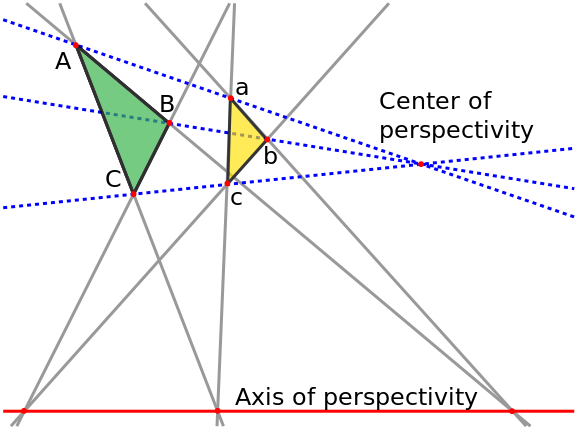
\includegraphics[width=.5\textwidth,height=.5\textheight,keepaspectratio]{DesarguesConfiguration.png}}
    \caption{Desargues-Konfiguration}
    \label{fig:Desargues}
  \end{figure}

  Analog zum Tetraeder, nur das die Inzidenzstruktur durch ${\mathcal{I}^5_{2, 3} = (\binom{[5]}{2}, \binom{[5]}{3}, \subseteq)}$ gegeben ist.
  Die Desargues-Konfi-guration ist selbstdual und hat 10 Punkte (Die Punkte $A, B, C, a, b, c$, das Zentrum der Perspektive und die drei Punkte, die auf der roten Linie liegen)
  und 10 Blöcke (Die 6 Linien der zwei Dreiecke, die 3 Linien, die sich im Zentrum der Perspektive treffen und die Achse der Perspektive).
  In der dazu dualen Konfiguration sind Achse und Zentrum der Perspektive getauscht.
\end{example}



\newpage

\section{Summation}

\begin{definition}
  Ein Paar $(S, \Sigma)$ heißt [finitäre] Summationsstruktur, falls $\Sigma$ eine Abbildungsvorschrift
  (Klassenabbildung) ist, die jeder Abbildung $\alpha \colon I \to S$ mit beliebiger [endlicher] Definitionsmenge $I$ 
  genau ein Element $\Sigma(\alpha)$ aus $S$ zuordnet, sodass gilt:
  \begin{itemize}
    \item Fundierungsaxiom: Ist $\alpha \colon \{ i \} \to S$, so gilt $\Sigma(\alpha) = \alpha(i)$.
    \item Teilsummenaxiom: Sind $\alpha \colon I \to S$ und $\eta \colon I \to A$ Abbildungen [$A$ und $I$ endlich],
          so gilt für die Abbildung $\beta \colon A \to S, a \mapsto \Sigma(\alpha_{\mid \eta^{-1}(a)})$
          stets: 
          \begin{equation*}
            \Sigma(\beta) = \Sigma(\alpha).
          \end{equation*}
  \end{itemize}
  Die Menge $S$ wird Grundmenge genannt.
\end{definition}

\begin{definition}
  Sei $(S, \Sigma)$ eine [finitäre] Summationsstruktur und ${\alpha \colon I \to S}$
  eine beliebige Abbildung [$I$ endlich]. 
  Dann gelten folgende Schreibweisen:
  \begin{itemize}
    \item $(\alpha(i))_{i \in I} = (\alpha(i) \mid i \in I) = \alpha$
    \item $\sum_{i \in I} \alpha(i) = \Sigma(\alpha)$
  \end{itemize}
\end{definition}

\begin{theorem}
  Sei $\Omega$ eine Menge. Dann ist $(\mathcal{P}(\Omega), \bigcup)$ eine Summationsstruktur,
  wobei für jede Abbildung $\alpha \colon I \to \mathcal{P}(\Omega)$ die Summation über $\alpha$ wie folgt
  definitert ist:
  \begin{equation*}
    \bigcup \alpha = \{ x \in \Omega \mid \exists i \in I \colon x \in \alpha(i) \}.
  \end{equation*}
\end{theorem}
\begin{proof}
  Sei $\alpha \colon \{ i' \} \to \mathcal{P}(\Omega)$ eine Abbildung.
  Es ist
  \begin{equation*}
    \bigcup \alpha = \{ x \in \Omega \mid \exists i \in \{i'\} \colon x \in \alpha(i) \}
    = \alpha(i').
  \end{equation*}
  Also gilt das Fundierungsaxiom.

  Seien nun $\alpha \colon I \to \mathcal{P}(\Omega)$ und $\eta \colon I \to A$ Abbildungen.
  Dann gilt für die Abbildung 
  $\beta \colon A \to \mathcal{P}(\Omega), a \mapsto \bigcup \alpha_{\mid \eta^{-1}(a)}$:
  \begin{align*}
    \beta(a) &= \{ x \in \Omega \mid \exists i \in \eta^{-1}(a) \colon x \in \alpha(i) \}.\\
    \bigcup \beta &= \{ x \in \Omega \mid \exists a \in A \colon x \in \beta(a) \}\\
    &= \{ x \in \Omega \mid \exists a \in A \exists i \in \eta^{-1}(a) \colon x \in \alpha(i) \}\\
    &= \{ x \in \Omega \mid \exists i \in I \colon x \in \alpha(i) \}\\
    &= \bigcup \alpha.
  \end{align*}
  Also gilt auch das Teilsummenaxiom.
\end{proof}

\begin{theorem}[Invarianz der Summation gegenüber Umbenennung]
  Sei $(S, \Sigma)$ eine [finitäre] Summationsstruktur.
  Sei außerdem $\alpha \colon I \to S$ eine Abbildung 
  und sei $\tau \colon H \to I$ eine Bijektion [$I$ endlich].
  Dann gilt:
  \begin{equation*}
    \Sigma(\alpha \circ \tau) = \Sigma(\alpha).
  \end{equation*}
\end{theorem}
\begin{proof}
  Sei $\eta = \tau^{-1}$ eine Abbildung von $I$ nach $H$.
  Weiterhin sei eine Abbildung $\beta \colon H \to S, h \mapsto \Sigma(\alpha_{\mid \{\eta^{-1}(h) \}})$ definiert.
  Aus dem Fundierungsaxiom folgt dann 
  \begin{align*}
    \beta(h) = \Sigma(\alpha_{\mid \{ \tau(h) \}}) = \alpha(\tau(h)) = (\alpha \circ \tau)(h).
  \end{align*}
  Also ist $\beta = {\alpha \circ \tau}$.
  Weiterhin gilt laut Teilsummenaxiom $\Sigma(\beta) = \Sigma(\alpha)$ und damit $\Sigma({\alpha \circ \tau}) = \Sigma(\alpha)$.
\end{proof}

\begin{definition}
  Sei $\mathbb{S} = (S, \Sigma)$ eine Summationsstruktur.
  Dann definieren wir $0_\mathbb{S} = \Sigma(\emptyset \to S)$.
\end{definition}

\begin{theorem}\label{Theorem_SumStrukturNeutral}
  Sei $\mathbb{S} = (S, \Sigma)$ eine Summationsstruktur
  und $f \colon A \to S, a \mapsto 0_\mathbb{S}$ eine konstante Abbildung.
  Dann gilt
  \begin{equation*}
    \Sigma(f) = 0_\mathbb{S}.
  \end{equation*}
\end{theorem}
\begin{proof}
  Sei $\alpha = \emptyset \to S$ eine Abbildung.
  Seien weiterhin die Abbildungen
  $\eta \colon \emptyset \to A$
  und $\beta \colon A \to S, a \mapsto \Sigma(\alpha_{\mid \eta^{-1}(a)})$ gegeben.
  Dann gilt laut dem Teilsummenaxiom
  \begin{equation*}
    0_\mathbb{S}
    = \Sigma(\alpha)
    = \Sigma(\beta)
    = \sum_{a \in A} \Sigma(\alpha_{\mid \eta^{-1}(a)})
    = \sum_{a \in A} \Sigma(\alpha_{\mid \emptyset})
    = \sum_{a \in A} 0_\mathbb{S}
    = \Sigma(f).
  \end{equation*}
\end{proof}

\begin{definition}
  Sei $\mathbb{S} = (S, \Sigma)$ eine Summationsstruktur.
  Dann ist für beliebige Abbildungen $\alpha \colon I \to S$
  \begin{equation*}
    \text{supp}_\mathbb{S}(\alpha) = \{i \in I \mid \alpha(i) \neq 0_\mathbb{S}\}
  \end{equation*}
  der Support von $\alpha$ in $\mathbb{S}$.
\end{definition}

\begin{theorem}
  Sei $\mathbb{S} = (S, \Sigma)$ eine Summationsstruktur.
  Dann gilt für alle Abbildungen $\alpha \colon I \to S$
  \begin{equation*}
    \Sigma(\alpha) = \Sigma(\alpha_{\mid \text{supp}_\mathbb{S}(\alpha)}).
  \end{equation*}
\end{theorem}
\begin{proof}
  Es seien 
  $\eta \colon \text{supp}_\mathbb{S}(\alpha) \to I, i \mapsto i$
  sowie $\beta \colon I \to S, i \mapsto \Sigma(\alpha'_{\mid \eta^{-1}(i)})$ Abbildungen,
  wobei $\alpha' = \alpha_{\mid \text{supp}_\mathbb{S}(\alpha)}$.
  Dann gilt laut dem Teilsummenaxiom
  \begin{equation*}
    \Sigma(\alpha_{\mid \text{supp}_\mathbb{S}(\alpha)})
    = \Sigma(\alpha')
    = \Sigma(\beta)
    = \sum_{i \in I} \sum_{j \in \eta^{-1}(i)} \alpha'(j)
    = \Sigma(\alpha).
  \end{equation*}
  Die letzte Gleichung gilt, weil für alle $i \in I$
  \begin{equation*}
    \alpha(i) = 
    \begin{cases}
      \sum_{j \in \eta^{-1}(i)} \alpha'(j) = \alpha(i) & i \in \text{supp}_\mathbb{S}(\alpha) \\
      \sum_{j \in \eta^{-1}(i)} \alpha'(j = \sum_{j \in \emptyset} \alpha(j) = 0_\mathbb{S} & i \notin \text{supp}_\mathbb{S}(\alpha).
    \end{cases}
  \end{equation*}
\end{proof}

\begin{definition}
  Sei $\mathbb{S} = (S, \Sigma)$ eine [finitäre] Summationsstruktur und $N$ eine Menge.
  Dann ist $\mathbb{S}^N = (S^N, \bar\Sigma)$ die $N$-fache Potenz von $\mathbb{S}$,
  wobei $\bar\Sigma$ für jede Abbildungsfamilie $(\alpha_i)_{i \in I} \in (S^N)^I$
  ($I$ [endliche] Menge) wie folgt definiert ist:
  \begin{equation*}
    \overline{\sum_{i \in I}} \alpha_i \colon N \to S, n \mapsto \sum_{i \in I}\alpha_i(n).
  \end{equation*}
\end{definition}

\begin{theorem}\label{Theorem_OmegaPotenzSumStruktur}
  Ist $\mathbb{S} = (S, \Sigma)$ eine Summationsstruktur und $N$ eine Menge.
  So ist auch $\mathbb{S}^N = (S^N, \bar\Sigma)$ eine Summationsstruktur.
\end{theorem}
\begin{proof}
  Sei $\alpha \colon \{i\} \to S^N$ eine Abbildung.
  Da das Fundierungsaxiom in $\mathbb{S}$ gilt,
  ist $\bar\Sigma(\alpha) \colon N \to S, n \mapsto \alpha_i(n)$
  und somit $\bar\Sigma(\alpha) = \alpha(i)$.
  Also gilt das Fundierungsaxiom in $\mathbb{S}^N$.

  Seien nun $\alpha \colon I \to S^N$, 
  $\eta \colon I \to A$
   und $\beta \colon A \to S^N, a \mapsto \bar\Sigma(\alpha_{\mid \eta^{-1}(a)})$ Abbildungen.
  Dann gilt für alle $n \in N$:
  \begin{align*}
    (\bar\Sigma(\beta))(n) &= \sum_{a \in A}(\beta(a))(n) \\
    &= \sum_{a \in A}(\bar\Sigma(\alpha_{\mid \eta^{-1}(a)}))(n) \\
    &= \sum_{a \in A}\sum_{i \in \eta^{-1}(a)}(\alpha(i))(n) \\
    &= \sum_{i \in I}(\alpha(i))(n) \\
    &= (\bar\Sigma(\alpha))(n),
  \end{align*}
  wobei die vorletzte Gleichung aus dem Teilsummenaxiom für $\mathbb{S}$ folgt.
\end{proof}

\begin{definition}
  Sei $\mathbb{S} = (S, \Sigma)$ eine finitäre Summationsstruktur und $N$ eine Menge.
  Dann ist $\mathbb{S}^{(N)} = (S^{(N)}, \bar\Sigma)$ die $N$-fache Kopotenz von $\mathbb{S}$,
  wobei 
  \begin{equation*}
    S^{(N)} = \{s \in S^N \mid \text{supp}_\mathbb{S}(s) \text{ endlich}\}
  \end{equation*}
  und $\bar\Sigma$ für jede Abbildungsfamilie $(\alpha_i)_{i \in I} \in (S^{(N)})^I$
  ($I$ endliche Menge) wie folgt definiert ist
  \begin{equation*}
    \overline{\sum_{i \in I}} \alpha_i \colon N \to S, n \mapsto \sum_{i \in I}\alpha_i(n).
  \end{equation*}
\end{definition}

\begin{theorem}\label{Theorem_OmegaKopotenzSumStruktur}
  Ist $\mathbb{S} = (S, \Sigma)$ eine finitäre Summationsstruktur und $N$ eine Menge.
  So ist auch $\mathbb{S}^{(N)} = (S^{(N)}, \bar\Sigma)$ eine finitäre Summationsstruktur.
\end{theorem}
\begin{proof}
  Das Gelten von Fundierungs- und Teilsummenaxiom lassen sich analog zu Satz \ref{Theorem_OmegaPotenzSumStruktur} beweisen.
  An dieser Stelle soll daher lediglich gezeigt werden,
  dass für alle Abbildungen $\alpha \in (S^{(N)})^I$
  mit endlicher Indexmenge $I$ gilt,
  dass $\text{supp}_\mathbb{S}(\bar\Sigma(\alpha))$ endlich ist,
  d.h. $\bar\Sigma(\alpha) \in S^{(N)}$.

  Der Support von $\bar\Sigma(\alpha)$ ist
  \begin{equation*}
    \text{supp}_\mathbb{S} \bigg( \overline{\sum_{i \in I}} \alpha_i \bigg)
    = \{n \in N \mid \sum_{i \in I} \alpha_i(n) \neq 0_\mathbb{S}\}.
  \end{equation*} 
  Ist $N$ endlich folgt die Aussage daher sofort.
  Sei $N$ also eine unendliche Menge.
  Aus Satz \ref{Theorem_SumStrukturNeutral} folgt,
  dass für alle $n \in \text{supp}_\mathbb{S}(\bar\Sigma(\alpha))$
  ein $i \in I$ existieren muss, sodass $\alpha_i(n) \neq 0_\mathbb{S}$.
  Für einen Widerspruch sei angenommen 
  $\text{supp}_\mathbb{S}(\bar\Sigma(\alpha))$ wäre unendlich.
  Da $I$ aber eine endliche Menge ist,
  muss es ein $j \in I$ gegeben,
  sodass $\alpha_j(n) \neq 0_\mathbb{S}$ für unendlich viele $n \in N$.
  Dies widerspricht aber der Voraussetzung,
  dass $\alpha_j \in S^{(N)}$. 
\end{proof}

\begin{definition}
  Seien $\mathbb{S} = (S, \Sigma)$ und $\mathbb{S}' = (S', \Sigma')$ Summationsstrukturen.
  Dann ist eine Abbildung $\varphi \colon S \to S'$ ein Homomorphismus von $\mathbb{S}$ nach $\mathbb{S}'$
  falls für jede Abbildung $\alpha \colon I \to S$ stets gilt:
  \begin{equation*}
    \varphi(\Sigma(\alpha)) = \Sigma'(\varphi \circ \alpha).
  \end{equation*}

  Ein bijektiver Homomorphismus wird Isomorphismus genannt.
\end{definition}

\begin{theorem}
  Seien $\mathbb{S} = (S, \Sigma)$, $\mathbb{S}' = (S', \Sigma')$ und $\mathbb{S}'' = (S'', \Sigma'')$ Summationsstrukturen.
  Seien weiterhin $\varphi \colon S \to S'$ und $\varphi' \colon S' \to S''$ Homomorphismen in die jeweilige Struktur.
  Dann ist $\varphi' \circ \varphi \colon S \to S''$ ein Homomorphismus von $\mathbb{S}$ nach $\mathbb{S}''$.
\end{theorem}
\begin{proof}
  Für eine Abbildung $\alpha \colon I \to S$ gilt:
  \begin{align*}
    (\varphi' \circ \varphi)(\Sigma(\alpha)) &= \varphi'(\varphi(\Sigma(\alpha))) \\
    &= \varphi'(\Sigma'(\varphi \circ \alpha)) 
    = \Sigma''((\varphi' \circ \varphi) \circ \alpha).
  \end{align*}
\end{proof}

\begin{definition}
  Sei $\mathbb{S}$ eine Summationsstruktur. 
  Ein Homomorphismus von $\mathbb{S}$ nach $\mathbb{S}$ heißt Endomorphismus von $\mathbb{S}$.

  $\text{End}_\mathbb{S}$ bezeichnet die Menge aller Endomorphismen auf $\mathbb{S}$.
\end{definition}

\begin{definition}
  Eine [finitäre] Summationsstruktur $(S, \Sigma)$ heißt idempotent, falls für jede konstante Abbildung
  $\alpha \colon I \to S$ [wobei $I$ endlich] gilt:
  \begin{equation*}
    \forall i \in I \colon \Sigma(\alpha) = \alpha(i).
  \end{equation*}
\end{definition}

\begin{theorem}\label{Theorem_IdempotentSurjektion}
  Sei $(S, \Sigma)$ eine Summationsstruktur. Dann ist $(S, \Sigma)$ genau dann idempotent, 
  wenn für jede Abbildung $\alpha \colon I \to S$ und jede surjektive Abbildung $\tau \colon H \to I$ gilt:
  $\Sigma(\alpha \circ \tau) = \Sigma(\alpha)$.
\end{theorem}
\begin{proof}
  Zunächst sei angenommen, dass $(S, \Sigma)$ idempotent ist.
  Setze $\eta = \tau$. Dann ist $\beta \colon I \to S, i \mapsto \Sigma((\alpha \circ \tau)_{\mid \tau^{-1}(i)})$
  und es gilt $\Sigma(\alpha \circ \tau) = \Sigma(\beta)$ laut dem Teilsummenaxiom.
  $(\alpha \circ \tau)_{\mid \tau^{-1}(i)}$ ist eine konstante Abbildung,
  weshalb wegen der Idempotenz von $(S, \Sigma)$ für alle $h \in \tau^{-1}(i)$ gilt: 
  \begin{equation*}
    \Sigma((\alpha \circ \tau)_{\mid \tau^{-1}(i)}) = (\alpha \circ \tau)(h) = \alpha(i).
  \end{equation*}
  Das heißt $\alpha = \beta$ und somit $\Sigma(\alpha \circ \tau) = \Sigma(\beta) = \Sigma(\alpha)$.

  Gilt nun umgekehrt $\Sigma(\alpha \circ \tau) = \Sigma(\alpha)$ für jede Abbildung $\alpha \colon I \to S$ und jede surjektive Abbildung $\tau \colon H \to I$.
  Sei weiterhin für ein beliebiges $c \in S$ $\gamma \colon H \to S, h \mapsto c$ eine konstante Abbildung.
  Für ein festes $j \in H$ seien außerdem $\tau \colon H \to \{j\}, h \mapsto j$ und $\alpha \colon \{j\} \to S, j \mapsto c$ Abbildungen.
  Da $\gamma = \alpha \circ \tau$ und $\tau$ eine surjektive Abbildung ist gilt laut Voraussetzung
  für alle $h \in H$:
  \begin{equation*}
    \Sigma(\gamma) = \Sigma(\alpha \circ \tau) = \Sigma(\alpha) = c = \gamma(h),
  \end{equation*}
  wobei die vorletzte Gleichung aus dem Fundierungsaxiom folgt.
\end{proof}

\subsection{Summationsstrukturen und Monoide}

\begin{theorem}\label{Theorem_SummationMonoid}
  Sei $(M, \Sigma)$ eine [finitäre] Summationsstruktur.
  Dann lässt sich wie folgt das zu $(M, \Sigma)$ zugehörige kommutative Monoid $\mathbb{M} = (M, +, 0)$ konstruieren:
  Setze $0 = \Sigma(\emptyset \to M)$ und
  $+ \colon M \times M \to M, (a, b) \mapsto \Sigma(\alpha)$, wobei
  $\alpha \colon [2] \to M, \{ 1 \mapsto a, 2 \mapsto b\}$.
\end{theorem}
\begin{proof}
  Zunächst soll gezeigt werden, dass $\mathbb{M}$ assoziativ ist.
  Dazu sei $a,b,c \in M$. Weiterhin seien folgende Funktionen definiert:
  \begin{align*}
    \alpha &\colon [3] \to M, \{ 1 \mapsto a, 2 \mapsto b, 3 \mapsto c \},\\
    \eta_1 &\colon [3] \to [2], \{ 1 \mapsto 1, 2 \mapsto 1, 3 \mapsto 2 \},\\
    \eta_2 &\colon [3] \to [2], \{ 1 \mapsto 1, 2 \mapsto 2, 3 \mapsto 2 \}.
  \end{align*}
  Daraus ergeben sich 
  \begin{align*}
    \beta_1 &\colon [2] \to M, i \mapsto \Sigma(\alpha_{\mid \eta_1^{-1}(i)}) \text{ und}\\
    \beta_2 &\colon [2] \to M, i \mapsto \Sigma(\alpha_{\mid \eta_2^{-1}(i)}).
  \end{align*}
  Da $\beta_1$ eine Funktion von $[2] \to M$ ist kann $\Sigma(\beta_1)$ wie folgt dargestellt werden:
  \begin{align*}
    \Sigma(\beta_1) = \beta_1(1) + \beta_1(2).
  \end{align*}
  $\beta_1(1)$ ergibt sich aus folgender Gleichungskette:
  \begin{align*}
    \beta_1(1) &= \Sigma(\alpha_{\eta_1^{-1}(1)})\\
    &= \Sigma(\alpha_{[2]})\\
    &= \Sigma_{i \in [2]}(\alpha(i))\\ 
    &= \alpha(1) + \alpha(2) = a + b.
  \end{align*}
  $\beta_1(2)$ kann dagegen wie folgt berechnet werden:
  \begin{align*}
    \beta_1(2) = \Sigma(\alpha_{\mid \eta_1^{-1}(2)})
    = \Sigma(\alpha_{\mid \{3\}})
    = \alpha(3) = c
  \end{align*}
  Insgesamt ist also $\Sigma(\beta_1) = (a + b) + c$.
  
  Analog zu $\beta_1$ kann auch $\Sigma(\beta_2)$ wie folgt angegeben werden:
  \begin{align*}
    \Sigma(\beta_2) = \beta_2(1) + \beta_2(2).
  \end{align*}
  $\beta_2(1)$ ist schlicht:
  \begin{align*}
    \beta_2(1) = \Sigma(\alpha_{\mid \eta_2^{-1}(1)}) = \alpha(1) = a.
  \end{align*}
  Für $\beta_2(2)$ ergibt sich:
  \begin{align*}
    \beta_2(2) &= \Sigma(\alpha_{\mid \eta_2^{-1}(2)}) 
    = \Sigma(\alpha_{\mid \{2, 3\}}).
  \end{align*}
  Da $\alpha_{\mid\{2, 3\}}$ keine Abbildung von $[2] \to M$ ist bedarf es folgender Umbenennung:
  \begin{align*}
    \tau \colon [2] \to \{ 2, 3\}, \{ 1 \to 2, 2 \to 3 \}.
  \end{align*}
  Nun kann $\beta_2(2)$ wie folgt ausgedrückt werden:
  \begin{align*}
    \beta_2(2) &= \Sigma(\alpha_{\mid \{2, 3\}})\\
    &= \Sigma(\alpha_{\mid \{2, 3\}} \circ \tau)\\
    &= (\alpha_{\mid \{ 2,3\}} \circ \tau)(1) + (\alpha_{\mid \{ 2,3\}} \circ \tau)(2)\\
    &= \alpha(2) + \alpha(3)\\
    &= b + c.
  \end{align*}
  Also ist $\Sigma(\beta_2) = \beta_2(1) + \beta_2(2) = a + (b + c)$.

  Nach Teilsummenaxiom gilt schließlich:
  \begin{align*}
    \Sigma(\beta_1) = \Sigma(\alpha) = \Sigma(\beta_2).
  \end{align*}
  und damit
  \begin{align*}
    (a + b) + c = a + (b + c).
  \end{align*}
  
  Als nächstes soll gezeigt werden, dass $0$ tatsächlich das neutrale Element ist.
  Dazu sei $m \in M$ ein beliebiges Element aus $M$ und weiterhin seien folgende Funktionen definiert:
  \begin{align*}
    \alpha &\colon \{ 1 \} \to \{ m \}, 1 \mapsto m\\
    \eta_1 &\colon \{ 1 \} \to [2], 1 \mapsto 1\\
    \eta_2 &\colon \{ 1 \} \to [2], 1 \mapsto 2
  \end{align*}
  Daraus ergeben sich folgende Funktionen:
  \begin{align*}
    \beta_1 &\colon [2] \to M, i \mapsto \Sigma(\alpha_{\mid \eta_1^{-1}(i)}) \text{ und} \\
    \beta_2 &\colon [2] \to M, i \mapsto \Sigma(\alpha_{\mid \eta_2^{-1}(i)}).
  \end{align*}
  Es gelten
  \begin{align*}
    \Sigma(\beta_1) &= \beta_1(1) + \beta_1(2) \text{ und}\\
    \Sigma(\beta_2) &= \beta_2(1) + \beta_2(2).
  \end{align*}
  Weiterhin ist
  \begin{align*}
    \beta_1(1) &= \Sigma(\alpha_{\mid \eta_1^{-1}(1)}) = \Sigma(\alpha_{\mid \{1\}}) = \alpha(1) = m \text{ und}\\
    \beta_1(2) &= \Sigma(\alpha_{\mid \eta_1^{-1}(2)}) = \Sigma(\alpha_{\mid \emptyset}) = 0.
  \end{align*}
  Außerdem ist
  \begin{align*}
    \beta_2(1) &= \Sigma(\alpha_{\mid \eta_2^{-1}(1)}) = 0 \text{ und}\\
    \beta_2(2) &= \Sigma(\alpha_{\mid \eta_2^{-1}(2)}) = \alpha(1) = m.
  \end{align*}
  Laut Teilsummenaxiom gilt schließlich:
  \begin{align*}
    \Sigma(\beta_1) = \Sigma(\alpha) = \Sigma(\beta_2).
  \end{align*}
  und damit
  \begin{align*}
    m + 0 = m = 0 + m.
  \end{align*}
  
  Um letztendlich die Kommutativität zu zeigen seien $a,b \in M$ zwei Elemente aus $M$ und 
  folgende Funktionen definiert:
  \begin{align*}
    \alpha &\colon [2] \to M, \{ 1 \mapsto a, 2 \mapsto b\} \text{ und}\\
    \tau &\colon [2] \to [2], \{ 1 \mapsto 2, 2 \mapsto 1 \}.
  \end{align*}
  Laut Umbenennungssatz gilt:
  \begin{align*}
    a + b &= \alpha(1) + \alpha(2)\\
    &= \Sigma(\alpha)\\
    &= \Sigma(\alpha \circ \tau)\\
    &= (\alpha \circ \tau)(1) + (\alpha \circ \tau)(2)\\
    &= \alpha(\tau(1)) + \alpha(\tau(2)) = \alpha(2) + \alpha(1) = b + a.
  \end{align*}
  Damit ist die Behauptung bewiesen.
\end{proof}

\begin{definition}
  Sei $\mathbb{M} = (M, +, \varepsilon)$ ein  kommutatives Monoid.
  Dann ist $(M, \Sigma^\text{fin})$ die zu $\mathbb{M}$ gehörige finitäre Summationsstruktur,
  wobei für jede endliche Menge $I = \{i_1, i_2, \dots, i_n\}$
  und jede Abbildung $\alpha \colon I \to M$ 
  \begin{equation*}
    \Sigma^\text{fin}(\alpha) = \alpha(i_1) + \alpha(i_2) + \dots + \alpha(i_n).
  \end{equation*}
\end{definition}

\begin{theorem}
  Sei $\mathbb{M} = (M, +, \varepsilon)$ ein  kommutatives Monoid.
  Dann ist $(M, \Sigma^\text{fin})$ eine finitäre Summationsstruktur.
\end{theorem}
\begin{proof}
  Sei $\alpha \colon \{i\} \to M$ eine Abbildung.
  Dann ist $\Sigma^\text{fin}(\alpha) = \alpha(i)$.
  Es gilt demnach das Fundierungsaxiom.

  Seien weiterhin $\alpha \colon I \to M$,
  $\eta \colon I \to A$ und $\beta \colon A \to M, a \mapsto \Sigma^\text{fin}(\alpha_{\mid \eta^{-1}(a)})$
  Abbildungen, wobei $I = \{i_1, i_2, \dots, i_n\}$ und $A = \{a_1, a_2, \dots, a_m\}$ endliche Mengen sind.
  Außerdem sei $n_k = |\{ i_{k,l} \mid i_{k,l} \in \eta^{-1}(a_k) \subseteq I \}|$
  Dann ist 
  \begin{align*}
    \Sigma^\text{fin}(\beta)
    &= \beta(a_1) + \dots + \beta(a_m) \\
    &= (\alpha(i_{1,1}) + \dots + \alpha(i_{1,n_1})) + \dots + (\alpha(i_{m,1}) + \dots + \alpha(i_{m,n_m})) \\
    &= \alpha(i_1) + \dots + \alpha(i_n) \\
    &= \Sigma^\text{fin}(\alpha).
  \end{align*}
  Also gilt auch das Teilsummenaxiom.
\end{proof}

\begin{definition}
  Ein kommutatives Monoid $\mathbb{M} = (M, +, \varepsilon)$ heiße natürlich geordnet,
  falls $\leq_\mathbb{M} = \{ (x, y) \in M^2 \mid \exists t \in M \colon x + t = y \}$ eine Ordnungsrelation definiert.
\end{definition}

\begin{theorem}
  Sei $\mathbb{M} = (M, +, \varepsilon)$ ein kommutatives Monoid.
  Dann ist $\mathbb{M}$ genau dann natürlich geordnet wenn gilt:
  \begin{equation*} \label{EquationAntisymmetrischesMonoid}
    \forall x,s,t \in M \colon (x + s) + t = x \implies x + s = x.\tag{$\ast$}
  \end{equation*}
\end{theorem}
\begin{proof}
  Ist $\mathbb{M} = (M, +, \varepsilon)$ ein kommutatives Monoid, so ist $(M, \leq_\mathbb{M})$ stets reflexiv und transitiv.
  Denn für alle $x$ existiert $\varepsilon \in M$ mit $x + \varepsilon = x$ und somit $x \leq_\mathbb{M} x$.
  Gilt außerdem $x \leq_\mathbb{M} y$ und $y \leq_\mathbb{M} z$, d.h. ist $x + t_1 = y$ und $y + t_2 = z$ für $t_1, t_2 \in M$. 
  Dann ist $x + (t_1 + t_2) = z$, wobei $t_1 + t_2 \in M$, womit $x \leq_\mathbb{M} z$ gilt.

  Also bleibt zu zeigen, dass $(M, \leq_\mathbb{M})$ genau dann anti-symmetrisch ist wenn \eqref{EquationAntisymmetrischesMonoid} gilt.
  Sei dazu $(M, \leq_\mathbb{M})$ anti-symmetrisch und sei außerdem $(x + s) + t = x$ für beliebige $x,s,t \in M$.
  Dann ist $x \leq_\mathbb{M} x+ s$ und $x + s \leq_\mathbb{M} x$, also $x = x + s$.

  Gilt umgekehrt \eqref{EquationAntisymmetrischesMonoid} und seien $x,y \in M$ mit $x \leq_\mathbb{M} y$ und $y \leq_\mathbb{M} x$.
  Das heißt es existiert $t_1, t_2 \in M$ mit $x + t_1 = y$ und $y + t_2 = x$.
  Also ist $(x + t_1) + t_2 = x$, woraus laut Voraussetzung $x + t_1 = x$, also $y = x$, folgt.
\end{proof}

\begin{example}
  Beispiele für ein natürlich geordnetes kommutatives Monoid sind $(\mathbb{N}, +, 0)$ und $(\mathbb{R}_{\geq 0} \cup \{\infty\}, +, 0)$, wobei
  $x + \infty = \infty$.

  Ein Gegenbeispiel ist $(\mathbb{Z}, +, 0)$, da $0 \leq 1$ und $1 \leq 0$ gilt.
\end{example}

\begin{definition}
  Sei $(M, +, \varepsilon)$ ein Monoid. 
  Ein Element $x \in M$ heißt idempotent, falls
  \begin{equation*}
    x + x = x.
  \end{equation*}
  
  Ein Monoid heißt idempotent, falls jedes seiner Elemente idempotent ist.
\end{definition}

\begin{theorem}\label{Theorem_IdempotentSumMonoid}
  Ein kommutatives Monoid $\mathbb{M}$ ist genau dann idempotent, 
  wenn die zu $\mathbb{M}$ gehörige finitäre Summationsstruktur idempotent ist.
\end{theorem}
\begin{proof}
  Sei $\mathbb{M} = (M, +, \varepsilon)$ ein idempotentes kommutatives Monoid.
  Sei weiterhin $\alpha \colon I \to M$ eine Abbildung mit endlicher Indexmenge $I = \{i_1, \dots, i_n\}$,
  sodass $\forall 1 \leq j \leq n \colon \alpha(i_j) = m \in M$.
  Dann ist für alle $i \in I$
  \begin{align*}
    \Sigma^\text{fin}(\alpha) &= \sum_{j = 1}^n\alpha(i_j) \\
    &= \sum_{j = 1}^n m = m = \alpha(i).
  \end{align*}
  Sei umgekehrt $(M, \Sigma^\text{fin})$ eine idempotente Summationsstruktur und $m \in M$ ein Element aus der Grundmenge.
  Weiterhin sei $\alpha \colon [2] \to M, i \mapsto m$ eine konstante Abbildung.
  Es gilt
  \begin{align*}
    m + m &= \alpha(1) + \alpha(2) = \Sigma^\text{fin}(\alpha) = m.
  \end{align*}
\end{proof}

\subsection{Summation und Inzidenzstrukturen}

\begin{definition}
  Eine Matrix über einer Menge $M$ (auch $M$-wertige Matrix) ist definitert als Tripel $(P, B, \alpha)$
  bestehend aus den Mengen $P$, $B$ und einer Abbildung $\alpha \colon P \times B \to M$.
  
  Wir sagen auch, dass $\alpha$ eine $(P \times B)$-Matrix über M ist. 
\end{definition}

\begin{definition}
  Eine $M$-wertige Matrix $\mathcal{I} = (P, B, \alpha)$ wird auch Fuzzy-Inzidenz-struktur genannt.
  Ist $\mathbb{M} = (M, \Sigma)$ eine [finitäre] Summationsstruktur, 
  so nennt man $\mathcal{I}$ auch eine Fuzzy-Inzidenzstruktur über $\mathbb{M}$.
  Sind $P$ und $B$ endlich, so ist $\mathcal{I}$ finitär.
\end{definition}

\begin{definition}
  Gegeben sei eine $M$-wertige Matrix $\mathcal{I} = (P, B, \alpha)$.
  Für jedes $p \in P$ heiße die Abbildung $\alpha(p, \cdot) \colon B \to M, b \mapsto \alpha(p, b)$
  die $p$-te Zeile von $\mathcal{I}$ bzw. $\alpha$.
  $\text{row}_\alpha \colon P \to M^B, p \mapsto \alpha(p, \cdot)$ ist die Row-Map für $\mathcal{I}$ bzw. $\alpha$.

  Analog wird für jedes $b \in B$ die Abbildung $\alpha(\cdot, b) \colon P \to M, p \mapsto \alpha(p, b)$
  als die $b$-te Spalte von $\mathcal{I}$ bzw. $\alpha$ bezeichnet.
  Weiterhin ist $\text{col}_\alpha \colon B \to M^P, b \mapsto \alpha(\cdot, b)$ die Column-Map für $\mathcal{I}$ bzw. $\alpha$.
\end{definition}

\begin{definition}
  Sei $\mathcal{I} = (P, B, \alpha)$ eine $M$-wertige Fuzzy-Inzidenzstruktur über $\mathbb{M} = (M, \Sigma)$.
  Dann ist die Zeilensumme von $\mathcal{I}$ bzw. $\alpha$
  \begin{equation*}
    \Sigma(\alpha(p, \cdot)) = \sum_{b \in B}\alpha(p, b).
  \end{equation*}
  Analog ist die Spaltensumme von $\mathcal{I}$ bzw. $\alpha$ definiert als
  \begin{equation*}
    \Sigma(\alpha(\cdot, b)) = \sum_{p \in P}\alpha(p, b).
  \end{equation*}
\end{definition}

\begin{definition}
  Eine Fuzzy-Inzidenzstruktur $\mathcal{I}$ über $\mathbb{M}$ wird als taktische Fuzzy-Konfiguration über $\mathbb{M}$ bezeichnet,
  falls $r_\mathcal{I}$ und $k_\mathcal{I}$ existieren mit
  \begin{itemize}
    \item $\forall p \in P  \colon \Sigma(\alpha(p, \cdot)) = r_\mathcal{I}$ und
    \item $\forall b \in B  \colon \Sigma(\alpha(\cdot, b)) = k_\mathcal{I}$.
  \end{itemize}
\end{definition}

\begin{theorem}[Satz der doppelten Abzählung]
  Sei  $\mathcal{I} = (P, B, \alpha)$ eine [finitäre] Fuzzy-Inzidenzstruktur über einer [finitären]
  Summationsstruktur $\mathbb{M} = (M, \Sigma)$.
  Dann gilt:
  \begin{equation*}
    \sum_{p \in P}\sum_{b \in B}\alpha(p, b) = \Sigma(\alpha) = \sum_{b \in B}\sum_{p \in P}\alpha(p, b).
  \end{equation*}
\end{theorem}
\begin{proof}
  Es seien $\eta \colon P \times B \to P, (p, b) \mapsto p$ und
  $\beta \colon P \to M, p \mapsto \Sigma(\alpha_{\mid \eta^{-1}(p)})$ Abbildungen.
  Desweiteren sei eine bijektive Abbildung $\tau_p \colon B \to \{p\} \times B, b \mapsto (p, b)$ gegeben.
  Für ein $p \in P$ ist
  \begin{align*}
    \beta(p) &= \Sigma(\alpha_{\mid \eta^{-1}(p)}) \\
    &= \Sigma(\alpha_{\mid \{p\} \times B}) \\
    &= \Sigma(\alpha_{\mid \{p\} \times B} \circ \tau_p) \\
    &= \Sigma(\alpha(p, \cdot)).
  \end{align*}
  Damit ergibt sich mithilfe des Teilsummenaxioms:
  \begin{align*}
    \sum_{p \in P}\sum_{b \in B}\alpha(p, b) &= \sum_{p \in P}\Sigma(\alpha(p, \cdot)) \\
    &= \sum_{p \in P}\beta(p) \\
    &= \Sigma(\alpha).
  \end{align*}
  Analog kann ebenfalls $\sum_{b \in B}\sum_{p \in P}\alpha(p, b) = \Sigma(\alpha)$ gezeigt werden.
\end{proof}

\begin{definition}
  Sei $\mathcal{I} = (P, B, I)$ eine Inzidenzstruktur.
  Sei weiterhin
  \begin{equation*}
    \alpha_{\mathcal{I}} \colon P \times B \to \mathbb{N} \cup \{\infty\}, (p, b) \mapsto
    \begin{cases}
      1 & p \mathrel{I} b \\
      0 & sonst
    \end{cases}
  \end{equation*}
  Dann ist $(P, B, \alpha_{\mathcal{I}})$ eine Fuzzy-Inzidenzstruktur über $(\mathbb{N} \cup \{\infty\}, \Sigma)$,
  wobei $\Sigma$ die erweiterte normale Summation darstellt.
\end{definition}

\begin{theorem}
  Eine endliche Inzidenzstruktur $\mathcal{I} = (P, B, I)$ ist genau dann eine taktische Konfiguration mit den Parametern $(|P|, r, |B|, k)$,
  wenn $\mathcal{I'} = (P, B, \alpha_{\mathcal{I}})$ eine taktische Fuzzy-Konfiguration mit den Parametern $(|P|, r_\mathcal{I}, |B|, k_\mathcal{I})$
  über der natürlichen Summationsstruktur $(\mathbb{N} \cup \{\infty\}, \Sigma)$ ist.
  Insbesondere ist $r = r_\mathcal {I}$ und $k = k_\mathcal{I}$.
\end{theorem}
\begin{proof}
  Sei $p \in P$ ein beliebiges Element in $P$.
  Dann gilt
  \begin{equation*}
    r_\mathcal{I} = \Sigma(\alpha_\mathcal{I}(p, \cdot)) 
    = \sum_{b \in B}\alpha_\mathcal{I}(p, b)
    = \sum_{b \in pI}1 = |pI| = r.
  \end{equation*}

  Ein ähnliches Argument kann auch für die Blöcke verwendet werden, wodurch die Behauptung bewiesen ist.
\end{proof}

\begin{theorem}
  Ist $\mathcal{I} = (P, B, \alpha)$ eine taktische Fuzzy-Konfiguration mit den Parametern $(|P|, r_\mathcal{I}, |B|, k_\mathcal{I})$ über der Summationsstruktur $\mathbb{M} = (M, \Sigma)$, so gilt:
  \begin{equation*}
    \sum_{p \in P}r_\mathcal{I} = \sum_{b \in B}k_\mathcal{I}.
  \end{equation*}
\end{theorem}
\begin{proof}
  Mithilfe der doppelten Abzählung ergibt sich:
  \begin{equation*}
    \sum_{p \in P}r_\mathcal{I} = \sum_{p \in P}\Sigma(\alpha(p, \cdot)) = \sum_{b \in B}\Sigma(\alpha(\cdot, b)) = \sum_{b \in B}k_\mathcal{I}.
  \end{equation*}  
\end{proof}

\newpage
\section{Targoide und vollständige Verbände}

\begin{definition}
  Sei $\mathbb{P} = (P, R)$ ein binäres Relat.
  Zu einer Teilmenge $X \subseteq P$ heiße $t \in P$ Target von $X$ bzgl. $\mathbb{P}$ falls
  $\forall x \in X \colon x \mathrel{R} t$.

  Analog heißt $s \in X$ Source von $X$ bzgl. $\mathbb{P}$ falls
  $\forall x \in X \colon s \mathrel{R} x$.
\end{definition}

\begin{definition}
  Sei $\mathbb{P} = (P, R)$ ein binäres Relat und $X \subseteq P$.
  Dann ist $t$ ein essentielles Target von $X$ bzgl. $\mathbb{P}$, falls es ein Target von $X$ ist
  und weiterhin gilt: 
  \begin{equation*}
    \forall u \in P \colon ((\forall x \in X \colon x \mathrel{R} u) \implies t \mathrel{R} u),
  \end{equation*}
  d.h. wenn $u \in P$ ebenfalls Target von $X$ ist, dann gilt $t \mathrel{R} u$.

  Analog dazu ist der Begriff essentielle Source definiert.
\end{definition}

\begin{definition}
  Ein binäres Relat $\mathbb{P} = (P, R)$ heißt Targoid falls
  jede Teilmenge $X \subseteq P$ ein essentielles Target besitzt (Targoid-Eigenschaft).

  Analog dazu heißt ein binäres Relat Sourcoid falls
  jede Teilmenge $X \subseteq P$ eine essentielle Source besitzt (Sourcoid-Eigenschaft).
\end{definition}

\begin{definition}
  Ist $\mathbb{P} = (P, R)$ ein binäres Relat,
  so ist $\mathbb{P}^{-1} = (P, R^{-1})$ mit $R^{-1} = \{ (q, p) \in R \mid p \mathrel{R} q \}$
  das dazu duale binäre Relat bzw. sein Opposite.
\end{definition}

\begin{theorem}
  Ein binäres Relat $\mathbb{P} = (P, R)$ ist ein Tagroid genau dann wenn
  $\mathbb{P}^{-1}$ ein Sourcoid ist.
\end{theorem}
\begin{proof}
  Sei $\mathbb{P} = (P, R)$ ein Targoid und $X \subseteq P$ eine beliebige Teilmenge.
  Ist $t \in P$ ein Target von $X$ bzgl. $\mathbb{P}$,
  dann gilt $x \mathrel{R} t$ für alle $x \in X$
  also auch $t \mathrel{R}^{-1} x$.
  Das heißt die Targets von $X$ bzgl. $\mathbb{P}$
  sind genau die Sources von $X$ bzgl. $\mathbb{P}^{-1}$.

  Sei nun $t \in P$ ein essentielles Target von $X$ bzgl. $\mathbb{P}$.
  Das heißt für alle weiteren Targets $u \in P$ bzgl. $\mathbb{P}$ gilt $t \mathrel{R} u$,
  also $u \mathrel{R}^{-1} t$.
  Da alle Targets von $X$ bzgl. $\mathbb{P}$ Sources von $X$ bzgl. $\mathbb{P}^{-1}$ sind,
  ist $t$ eine essentielle Source von $X$ bzgl. $\mathbb{P}^{-1}$.
\end{proof}

\begin{lemma}\label{Lemma_SuperSource}
  Sei $(P, R)$ ein Targoid mit nichtleerer Grundmenge $P$.
  Dann existiert ein Element $p \in P$ für das gilt: $\forall q \in P \colon p \mathrel{R} q$.
  Das heißt insbesondere, dass $p$ Source von jeder Teilmenge in $P$ ist.
\end{lemma}
\begin{proof}
  Sei $X = \emptyset \subseteq P$. Dann ist die Menge aller Targets von $X$ gleich der Menge $P \neq \emptyset$.
  Da $(P, R)$ ein Targoid ist, gibt es zu $X$ ein essentielles Target $t$.
  Das heißt, es gilt $t \mathrel{R} p$ für alle Targets $p$ von $X$, was aber allen Elementen in $P$ entspricht.
\end{proof}

\begin{theorem}\label{Theorem_TargoidEqualsSourcoid}
  Ein binäres Relat $\mathbb{P} = (P, R)$ ist ein Tagroid genau dann wenn
  $\mathbb{P}$ ein Sourcoid ist.
\end{theorem}
\begin{proof}
  Sei $\mathbb{P} = (P, R)$ ein Targoid und $X \subseteq P$ eine beliebige Teilmenge von $P$.
  Sei weiterhin $S_X = \{s \in P \mid s \text{ ist Source von } X\} \subseteq P$.
  $S_X$ ist wegen Lemma \ref{Lemma_SuperSource} nicht leer.
  Da $\mathbb{P}$ ein Targoid ist, existiert ein essentielles Target $t$ von $S_X$.
  Für alle $x \in X$ gilt: $x$ ist Target von $S_X$.
  Da $t$ ein essentielles Target ist gilt aber auch $t \mathrel{R} x$ für alle $x \in X$.
  Das heißt, dass $t$ eine Source von $X$ ist.
  Sei weiterhin $s \in P$ eine Source von $X$.
  Dann ist auch $s \in S_X$ und da $t$ ein Target von $S_X$ gilt $s \mathrel{R} t$.
  Also ist $t$ eine essentielle Source von $X$.

  Sei umgekehrt $\mathbb{P}$ ein Sourcoid.
  Dann ist $\mathbb{P}^{-1}$ ein Targoid und deshalb wie soeben gezeigt ein Sourcoid.
  Also ist $(\mathbb{P}^{-1})^{-1} = \mathbb{P}$ ein Targoid.
\end{proof}

\begin{figure}
  \centering {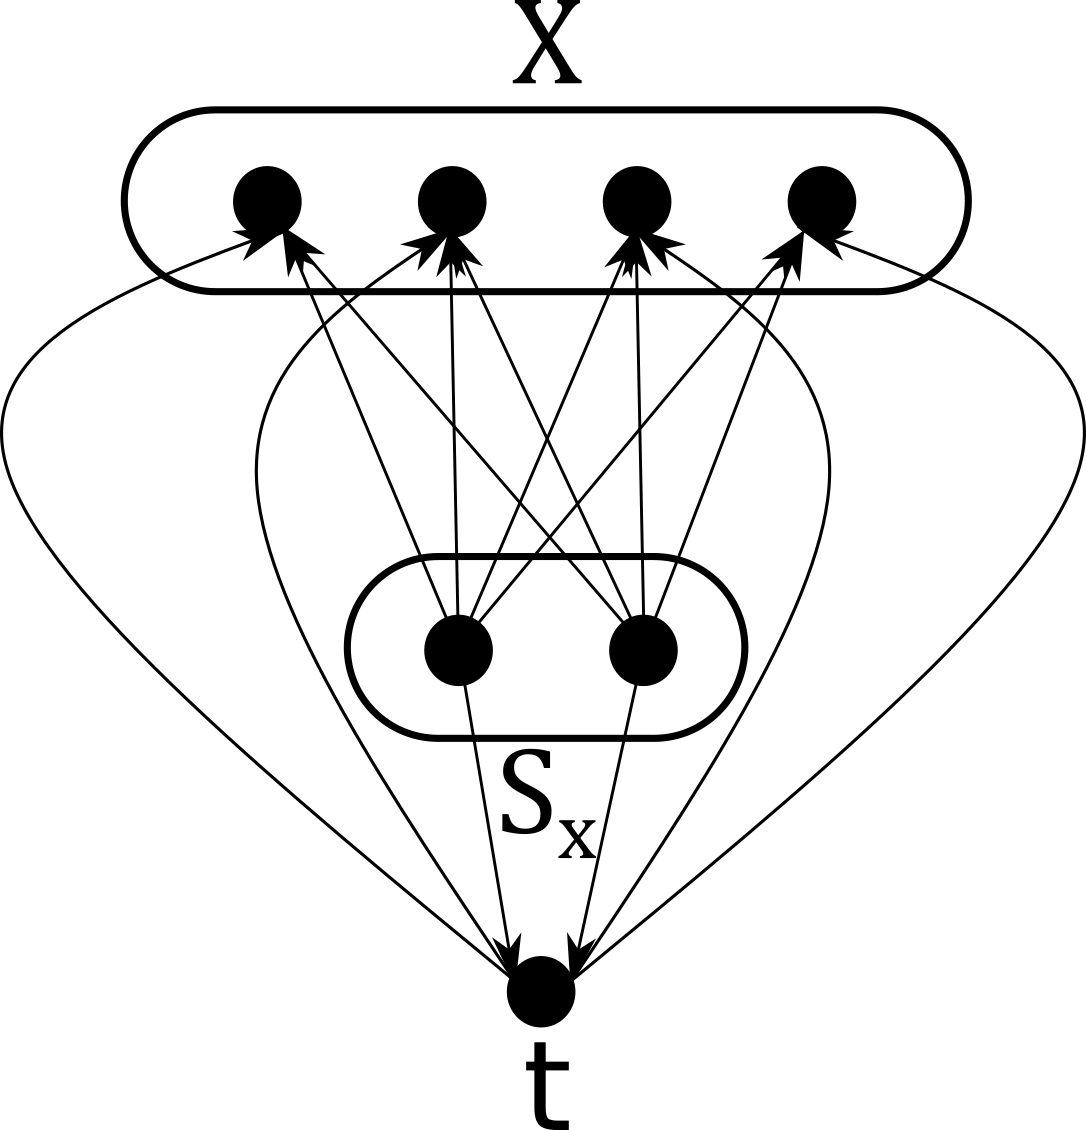
\includegraphics[width=.5\textwidth,height=.5\textheight,keepaspectratio]{TargoidSourcoid.png}}
  \caption{Veranschaulichung von Satz \ref{Theorem_TargoidEqualsSourcoid}}
  \label{fig:TargoidSourcoid}
\end{figure}

\subsection{vollständige Verbände und Summation}

\begin{definition}
  Ein binäres Relat $\mathbb{P} = (P, R)$ heißt vollständiger Verband (geordnetes Targoid), 
  falls $\mathbb{P}$ sowohl Ordnung als auch Targoid bzw. Sourcoid ist.
\end{definition}

\begin{theorem}\label{Theorem_ReflexivesRelat}
  Ist $(P, R)$ ein reflexives binäres Relat, 
  dann ist $p$ ein essentielles Target von $\{p\}$.
\end{theorem}
\begin{proof}
  Da $(p, p) \in R$ ist $p$ Target von $\{p\}$.
  Sei $t$ ein beliebiges Target von $\{p\}$.
  Dann gilt auch $p \mathrel{R} t$, womit bewiesen wäre, dass $p$ ein essentielles Target ist.
\end{proof}

\begin{theorem}\label{Theorem_AntisymmetrischesRelat}
  Ist $(P, R)$ anti-symmetrisch, so existiert zu jeder Teilmenge nur höchstens ein essentielles Target.
\end{theorem}
\begin{proof}
  Angenommen für eine Teilmenge von $P$ existieren zwei verschiedene essentielle Targets $t_1$ und $t_2$.
  Dann gilt aber auch $t_1 \mathrel{R} t_2$ und $t_2 \mathrel{R} t_1$ und wegen der 
  Anti-Symmetrie auch $t_1 = t_2$. Widerspruch.
\end{proof}

\begin{definition}
  Sei $(P, R)$ ein binäres Relat und sei $\alpha \colon I \to P$ eine Abbildung.
  Dann heiße $t \in P$ [essentielles] Target von $\alpha$ in $(P, R)$,
  falls $t$ ein [essentielles] Target von $\alpha(I)$ ist.
\end{definition}

\begin{lemma}\label{Lemma_TransitivesRelat}
  Sei $(P, R)$ ein transitives binäres Relat. Dann gilt:
  Sind $\alpha \colon I \to P$ und $\eta \colon I \to A$ Abbildungen derart, 
  dass für alle $a \in A$ zu $\alpha_{\mid \eta^{-1}(a)}$ stets ein essentielles Target $t_a$ existiert
  und ein $t \in P$ existiert, welches ein essentielles Target von $\alpha$ ist,
  so ist $t$ auch essentielles Target von $\beta \colon A \to P, a \mapsto t_a$.
\end{lemma}
\begin{proof}
  Da $t$ ein Target von $\alpha$ ist,
  ist $t$ auch gleichzeitig Target von $\alpha_{\mid \eta^{-1}(a)}$
  für alle $a \in A$.
  Da $t_a$ das essentielle Target von $\alpha_{\mid \eta^{-1}(a)}$ ist, ist auch $t_a \mathrel{R} t$.
  Das bedeutet, dass für alle $a \in A$ gilt: $\beta(a) \mathrel{R} t$, womit gezeigt wäre, 
  dass $t$ ein Target von $\beta$ in $(P, R)$ ist.

  Sei $u \in P$ ein weiteres Target von $\beta$ in $(P, R)$.
  Das heißt $\forall a \in A \colon t_a \mathrel{R} u$.
  Für jedes $a \in A$ ist $t_a$ aber auch Target von $\alpha_{\mid \eta^{-1}(a)}$,
  weshalb $\forall i \in \eta^{-1}(a) \colon \alpha(i) \mathrel{R} t_a$.
  Da $(P, R)$ transitiv ist gilt damit $\forall a \in A \forall i \in \eta^{-1}(a) \colon \alpha(i) \mathrel{R} u$
  und somit $\forall i \in I \colon \alpha(i) \mathrel{R} u$, d.h. $u$ ist Target von $\alpha$ in $(P, R)$.
  Da $t$ ein essentielles Target von $\alpha$ in $(P, R)$ ist, gilt $t \mathrel{R} u$.

  Damit ist die Behauptung bewiesen.
\end{proof}

\begin{figure}
  \centering {\includegraphics[width=0.75\textwidth,height=0.75\textheight,keepaspectratio]{transitivesRelat.png}}
  \caption{Veranschaulichung von Lemma \ref{Lemma_TransitivesRelat}}
  \label{fig:TransitivesRelat}
\end{figure}

\begin{definition}
  Sei $\mathbb{P} = (P, R)$ ein vollständiger Verband.
  Dann ist $\text{sup}_\mathbb{P}$ eine Klassenabbildung,
  die jeder Abbildung $\alpha \colon I \to P$
  das essentielle Target von $\alpha$ in $\mathbb{P}$ zuordnet.
  $\text{sup}_\mathbb{P}(\alpha)$ wird auch als das Supremum von $\alpha$ bezeichet.

  Analog ist die Klassenabbildung $\text{inf}_\mathbb{P}$ definiert,
  die jeder Abbildung $\alpha \colon I \to P$
  die essentielle Source von $\alpha$ in $\mathbb{P}$ zuordnet.
  $\text{inf}_\mathbb{P}(\alpha)$ wird auch als das Infimum von $\alpha$ bezeichet.
\end{definition}

\begin{theorem}\label{Theorem_VerbandSummationsstruktur}
  Ist $\mathbb{P} = (P, R)$ ein vollständiger Verband, 
  so ist $(P, \text{sup}_\mathbb{P})$
  eine idempotente Summationsstruktur.
\end{theorem}
\begin{proof}
  Sei $\alpha \colon \{i\} \to P$ eine Abbildung.
  Wegen der Reflexivität von $(P, R)$ besitzt $\alpha$ laut Satz \ref{Theorem_AntisymmetrischesRelat} genau ein essentielles Target,
  welches laut Satz \ref{Theorem_ReflexivesRelat} $\alpha(i)$ ist.
  Also ist $\text{sup}_\mathbb{P}(\alpha) = \alpha(i)$ und das Fundierungsaxiom gilt.

  Seien weiterhin $\alpha \colon I \to P$, $\eta \colon I \to A$
  und  $\beta \colon A \to P, a \mapsto \text{sup}_\mathbb{P}(\alpha_{\mid \eta^{-1}(a)})$ Abbildungen.
  Aufgrund der Antisymmetrie besitzt $\alpha$ genau ein essentielles Target $\text{sup}_\mathbb{P}(\alpha)$ in $(P, R)$ (Satz \ref{Theorem_AntisymmetrischesRelat}).
  Aus dem selben Grund besitzt $\alpha_{\mid \eta^{-1}(a)}$ für alle $a \in A$ ein essentielles Target $\text{sup}_\mathbb{P}(\alpha_{\mid \eta^{-1}(a)}) = \beta(a)$.
  Durch das soeben bewiesenen Lemma \ref{Lemma_TransitivesRelat} ergibt sich somit, 
  dass das essentielle Target von $\beta$ gleich dem essentiellen Target von $\alpha$ ist.
  Damit ist $\text{sup}_\mathbb{P}(\alpha) = \text{sup}_\mathbb{P}(\beta)$, womit gezeigt ist, dass auch das Teilsummenaxiom erfüllt ist.

  Zu zeigen bleibt also noch die Idempotenz.
  Dazu sei $\alpha \colon I \to P, i \mapsto p$ eine konstante Abbildung.
  $\sup_\mathbb{P}(\alpha)$ ist das (eindeutig bestimmte) essentielle Target von $\alpha(I) = \{p\}$.
  Dies entspricht laut Satz \ref{Theorem_ReflexivesRelat} $p$ selbst, also gilt für alle $i \in I$: $\sup_\mathbb{P}(\alpha) = p = \alpha(i)$.

\end{proof}

\begin{theorem}
  Ist $\mathbb{S} = (S, \Sigma)$ eine idempotente finitäre Summationsstruktur 
  und $+$ die durch $\mathbb{S}$ induzierte Addition, 
  so gilt für $\leq_\mathbb{S} = \{(x, y) \in S^2 \mid \exists s \in S \colon x + s = y\}$ stets,
  dass $(S, \leq_{\mathbb{S}})$ ein vollständiger Verband ist.
\end{theorem}
\begin{proof}
  Es gilt $x + 0_\mathbb{S} = x$ und damit $x \leq_\mathbb{S} x$ für alle $x \in X$.
  Ist außerdem $x \leq_\mathbb{S} y$ und $y \leq_\mathbb{S} z$ für $x, y, z \in S$,
  so gibt es $s_1, s_2 \in S$ mit $y = x + s_1$ und $z = y + s_2$
  und damit auch $z = x + (s_1 + s_2)$, also $x \leq_\mathbb{S} z$.
  Weiterhin ist $(S, +, 0)$ laut Satz \ref{Theorem_IdempotentSumMonoid} idempotent, da $\mathbb{S}$ idempotent ist.
  Seien $x, y \in S$ und gelte $x \leq_\mathbb{S} y$ und $y \leq_\mathbb{S} x$, d.h.
  es existieren $s_1, s_2 \in S$ mit $x + s_1 = y$ und $y + s_2 = x$. Dann gilt:
  \begin{equation*}
    y = x + s_1 = x + (x + s_1) = x + y = y + x = y + (y + s_2) = y + s_2 = x.
  \end{equation*}

  Zu zeigen bleibt also noch, dass jede Teilmenge von $S$ ein essentielles Target besitzt.
  Sei also $X \subseteq S$ eine Teilmenge von $S$ und $t = \text{max}(X)$.
  Dann ist $t$ das essentielle Target von $X$ und die Aussage ist bewiesen.
\end{proof}

\newpage
\section{Summoide}

\begin{definition}
  Ein Summoid ist definiert als Quadrupel $\mathcal{S} = (S, \Sigma, *, \varepsilon)$,
  bestehend aus einer Summationsstruktur $\mathcal{S}_\text{Sum} = (S, \Sigma)$ und 
  einem Monoid $\mathcal{S}_\text{Mult} = (S, *, \varepsilon)$, sodass
  für ein Element $s \in S$ und eine Abbildung $\alpha \colon I \to S$ folgende Distributivgesetze gelten:
  \begin{align*}
    s \ast \Sigma(\alpha) = \Sigma(s \ast \alpha) \text{ mit } s \ast \alpha \colon I \to S, i \mapsto s \ast \alpha(i) \\
    \Sigma(\alpha) \ast s = \Sigma(\alpha \ast s) \text{ mit } \alpha \ast s \colon I \to S, i \mapsto \alpha(i) \ast s
  \end{align*}
  Ein Summoid $\mathcal{S}$ heißt finitär wenn $\mathcal{S}_\text{Sum}$ eine finitäre Summationsstruktur ist.
\end{definition}

\begin{example}
  Sei $\Omega$ eine Menge. Dann ist $\mathcal{S}_\Omega = (\mathcal{P}(\Omega), \bigcup, \cap, \Omega)$ 
  das sogenannte Potenzmengensummoid.
\end{example}

\begin{example}
  Das Quadrupel $\mathcal{S}_\text{Real} = ([0, \infty], \Sigma, \ast, 1)$ ist das reelle Summoid,
  wobei $\Sigma(\alpha) = \sup_{J \subseteq_\text{fin} I}(\Sigma(\alpha_{\mid J}))$ für jede Abbildung $\alpha \colon I \to[0, \infty]$
  bzgl. der Ordnung $\leq$ mit $x \leq y \iff \exists t \in [0, \infty] \colon x + t = y$ und
  $\cdot$ die übliche Multiplikation darstellt mit $x \cdot \infty = \infty \cdot x = \infty$.
\end{example}

\begin{example}
  Das Quadrupel $\mathcal{S}_\text{trop} = ([0, \infty], \Sigma_\text{trop}, \cdot_\text{trop}, 1_\text{trop})$
  ist das reelle tropische Summoid, wobei für jede Abbildung $\alpha \colon I \to [0, \infty]$
  \begin{equation*}
    \Sigma_\text{trop}(\alpha) = \inf_{([0, \infty], \leq)}\alpha
  \end{equation*}
  und für $x, y \in [0, \infty]$
  \begin{equation*}
    x \cdot_\text{trop} y = 
    \begin{cases}
      x + y &\quad\text{falls } \infty \notin \{x, y\} \\
      \infty &\quad\text{sonst}
    \end{cases} 
  \end{equation*}
  sowie $1_\text{trop} = 0$.

  Achtung: $0_\text{trop} = \Sigma_\text{trop}(\emptyset \to [0, \infty]) = \infty$.
\end{example}

\begin{example}\label{Exmaple_Relationensummoid}
  Sei $P$ eine Menge. Dann ist $\text{Rel}_2P = (\mathcal{P}(P \times P), \bigcup, \ast, \Delta_P)$ mit
  $R \ast S = \{(p, q) \in P \times P \mid \exists t \in P \colon p \mathrel{R} t \wedge t \mathrel{S} q\}$
  sowie $\Delta_P = \{(p, p) \mid p \in P\}$ (die diagonale Gleichheitsrelation) ein Summoid,
  welches das Relationensummoid zu $P$ genannt wird.
\end{example}

\begin{theorem}
  Das Relationensummoid $\text{Rel}_2P = (\mathcal{P}(P \times P), \bigcup, \ast, \Delta_P)$ aus Beispiel \ref{Exmaple_Relationensummoid}
  ist ein Summoid.
\end{theorem}
\begin{proof}
  An dieser Stelle soll nur die Linksdistributivität gezeigt werden.
  Seien dazu $R \in \mathcal{P}(P \times P)$ und 
  $S \colon \Lambda \to \mathcal{P \times P}$ eine Abbildung für eine beliebige Indexmenge $\Lambda$.
  %$(S_\lambda)_{\lambda \in \Lambda} \in (\mathcal{P}(P \times P))^\Lambda$ für eine Indexmenge $\Lambda$.
  Für alle $(p, q) \in P \times P$ gilt: 
  \begin{align*}
    (p, q) \in R \ast \bigcup_{\lambda \in \Lambda}S_\lambda &\iff \exists t \in P \colon (p, t) \in R \wedge (t, q) \in \bigcup_{\lambda \in \Lambda}S_\lambda \\
    &\iff \exists t \in P \colon (p, t) \in R \wedge \exists \lambda \in \Lambda \colon (t, q) \in S_\lambda \\
    &\iff \exists \lambda \in \Lambda \exists t \in P \colon (p, t) \in R \wedge  (t, q) \in S_\lambda \\
    &\iff (p, q) \in \bigcup_{\lambda \in \Lambda}R \ast S_\lambda.
  \end{align*}
\end{proof}

\begin{definition}
  Wir setzen $0_\mathcal{S} = 0_{\mathcal{S}_\text{Sum}}$.
\end{definition}

\begin{definition}
  Ein Summoid $\mathcal{S}$ heißt kommutativ falls $\mathcal{S}_\text{Mult}$ kommutativ ist.
\end{definition}

\begin{definition}
  Sei $\mathbb{S} = (S, \Sigma)$ eine [finitäre] Summationsstruktur.
  Dann wird $\text{End}(\mathbb{S}) = (\text{End}_\mathbb{S}, \bar\Sigma, \circ, \text{id}_S)$ als [finitäres] Endomorphismen-Summoid bezeichnet,
  wobei $\bar\Sigma(\varphi)$ für eine Abbildung $\varphi \colon \Lambda \to \text{End}_\mathbb{S}$ definiert ist als
  \begin{equation*}
    \bar\Sigma(\varphi) \colon S \to S, s \mapsto \sum_{\lambda \in \Lambda}\varphi_\lambda(s).
  \end{equation*}
  Ist $\mathcal{S}$ ein Summoid,
  so ist $\text{End}_\mathcal{S} = \text{End}(\mathcal{S}_\text{Sum})$.
\end{definition}

\begin{theorem}\label{Theorem_SummationEndomorphismus}
  Sei $\mathbb{S} = (S, \Sigma)$ eine [finitäre] Summationsstruktur.
  Dann ist das Endomorphismen-Summoid $\text{End}(\mathbb{S}) = (\text{End}_\mathbb{S}, \bar\Sigma, \circ, \text{id}_S)$ ein Summoid.
\end{theorem}
\begin{proof}
  Zunächst soll gezeigt werden, dass $(\text{End}_\mathbb{S}, \bar\Sigma)$ eine Summationsstruktur ist.
  Laut Satz \ref{Theorem_OmegaPotenzSumStruktur} ist bewiesen, dass $(S^S, \bar\Sigma)$ eine Summationsstruktur darstellt,
  wodurch noch zu zeigen bleibt, dass für jede beliebige Abbildung $\varphi \colon \Lambda \to \text{End}_\mathbb{S}$
  gilt: $\bar\Sigma(\varphi) \in \text{End}_\mathbb{S}$. 
  Sei dazu $\alpha \colon I \to S$ eine Abbildung.
  Dann gilt:
  \begin{align*}
    (\bar\Sigma(\varphi))(\Sigma(\alpha)) 
    &= \sum_{\lambda \in \Lambda}\varphi_\lambda(\Sigma(\alpha)) \\
    &= \sum_{\lambda \in \Lambda}\Sigma(\varphi_\lambda \circ \alpha) \\ 
    &= \sum_{\lambda \in \Lambda}\sum_{i \in I}\varphi_\lambda(\alpha(i)) \\
    &= \sum_{i \in I}\sum_{\lambda \in \Lambda}\varphi_\lambda(\alpha(i)) \\
    &= \sum_{i \in I}(\bar\Sigma(\varphi))(\alpha(i)) \\
    &= \Sigma((\bar\Sigma(\varphi)) \circ \alpha).
  \end{align*}

  Wie man leicht sieht ist $(\text{End}_\mathbb{S}, \circ, \text{id}_S)$ ein Monoid, 
  sodass nur noch die Distributivgesetze gezeigt werden müssen.
  Seien dazu $\psi \in \text{End}_\mathbb{S}$, $\varphi \colon \Lambda \to \text{End}_\mathbb{S}$.
  Dann gilt für alle $s \in S$
  \begin{align*}
    \psi((\bar\Sigma(\varphi))(s))
    = \psi \bigg(\sum_{\lambda \in \Lambda}\varphi_\lambda(s) \bigg)
    = \sum_{\lambda \in \Lambda}(\psi \circ \varphi_\lambda)(s)
    = (\bar\Sigma(\psi \circ \varphi))(s)
  \end{align*}
  und
  \begin{align*}
    (\bar\Sigma(\varphi))(\psi(s))
    = \sum_{\lambda \in \Lambda}\varphi_\lambda(\psi(s))
    = \sum_{\lambda \in \Lambda}(\varphi_\lambda \circ \psi)(s)
    = (\bar\Sigma(\varphi\circ \psi))(s).
  \end{align*}
\end{proof}

\begin{definition}
  Seien $\mathcal{S} = (S, \Sigma, \ast, \varepsilon)$ und $\mathcal{S}' = (S', \Sigma', \ast', \varepsilon')$ Summoide.
  Dann heißt eine Abbildung $\varphi$ Homomorphismus von $\mathcal{S}$ nach $\mathcal{S}'$, falls
  $\varphi$ ein Homomorphismus von $\mathcal{S}_\text{Sum}$ nach $\mathcal{S}'_\text{Sum}$ und 
  ein Homomorphismus von $\mathcal{S}_\text{Mult}$ nach $\mathcal{S}'_\text{Mult}$ ist.

  Ist $\varphi$ zudem bijektiv, so heißt $\varphi$ Isomorphismus.
\end{definition}

\begin{theorem}
  $\mathcal{S} = ([0, 1], \inf, \cdot, 1)$ und $\mathcal{S}' = ([0, \infty], \sup, +, 0)$ sind isomorph.
\end{theorem}
\begin{proof}
  Sei $\varphi \colon [0, \infty] \to [0, 1], x \mapsto 2^{-x}$, wobei $2^{-\infty} = 0$.
  $\varphi$ ist bijektiv und es gilt für jede Abbildung $\alpha \colon I \to [0, \infty]$:
  \begin{equation*}
    \varphi(\sup(\alpha))= \inf(\varphi \circ \alpha).
  \end{equation*}
  Außerdem gilt für alle $a, b \in [0, \infty]$:
  \begin{equation*}
    \varphi(a + b) = 2^{-(a+b)} = \varphi(a) \cdot \varphi(b).
  \end{equation*}
\end{proof}

\begin{theorem}
  Ist $\mathcal{S} = (S, \Sigma, \ast, \varepsilon)$ ein [finitäres] Summoid, 
  so ist die Abbildung $\lambda \colon S \to \text{End}_{\mathcal{S}_\text{Sum}}, s \mapsto \lambda_s$ mit
  $\lambda_s \colon S \to S, x \mapsto s \ast x$ ein injektiver Homomorphismus von $\mathcal{S}$ nach 
  $\text{End}_\mathcal{S} = (\text{End}_{\mathcal{S}_\text{Sum}}, \bar\Sigma, \circ, \text{id}_S)$.
\end{theorem}
\begin{proof}
  Zunächst muss gezeigt werden, dass $\lambda$ wohldefiniert ist, 
  d.h. dass für alle $s \in S$ gilt: $\lambda_s \in \text{End}_{S_\text{Sum}}$.
  Sei dazu $\alpha \colon I \to S$ eine Abbildung und $s \in S$. Dann ist 
  \begin{equation*}
    \lambda_s(\Sigma(\alpha)) = s \ast \Sigma(\alpha) = \Sigma(s \ast \alpha) = \Sigma(\lambda_s \circ \alpha).
  \end{equation*}

  Sei nun $\alpha \colon I \to S$ eine Abbildung mit [endlicher] Indexmenge $I$ und $s \in S$.
  Dann gilt 
  \begin{align*}
    (\lambda(\Sigma(\alpha)))(s)
    &= \lambda_{\Sigma(\alpha)}(s) \\
    &= \Sigma(\alpha) \ast s \\
    &= \Sigma(\alpha \ast s) \\
    &= \sum_{i \in I}(\alpha \ast s)(i) \\
    &= \sum_{i \in I}(\alpha(i) \ast s) \\
    &= \sum_{i \in I}((\lambda \circ \alpha)(i))(s)
    = (\bar\Sigma(\lambda \circ \alpha))(s).
  \end{align*}
  Seien nun $s_1, s_2, s \in S$.
  Dann ist
  \begin{align*}
    (\lambda(s_1 \ast s_2))(s)
    &= (s_1 \ast s_2) \ast s \\
    &= s_1 \ast (s_2 \ast s) \\
    &= s_1 \ast \lambda_{s_2}(s) \\
    &= \lambda_{s_1}(\lambda_{s_2}(s))
    = (\lambda(s_1) \circ \lambda(s_2))(s).
  \end{align*}
  Damit ist gezeigt, dass $\lambda$ ein Homomorphismus von $\mathcal{S}$ nach $\text{End}_\mathcal{S}$ ist.

  Um noch schließlich die Injektivität zu zeigen seien $s, t \in S$ und $\lambda(s) = \lambda(t)$.
  Dann gilt
  \begin{equation*}
    s = s \ast \varepsilon = \lambda_s(\varepsilon) = \lambda_t(\varepsilon) = t \ast \varepsilon = t. 
  \end{equation*}
\end{proof}

\begin{example}
  Sei $\text{Nat} = (\mathbb{N}, \Sigma, \cdot, 1)$ das natürliche Summoid.
  Dann ist \\$End(\text{Nat}_\text{Sum}) = (End_{\text{Nat}_\text{Sum}}, \bar\Sigma, \circ, \text{id}_\mathbb{N})$ das zur natürlichen Summationsstruktur gehörige Endomorphismen-Summoid.

  Sei $\mathbbm{1}^{[n]} \colon [n] \to \mathbb{N}, i \mapsto 1$ für jedes $n \in \mathbb{N}$.
  Dann gilt für jedes $\varphi \in End_{\text{Nat}_\text{Sum}}$:
  \begin{equation*}
    \varphi(n) = \varphi(\Sigma(\mathbbm{1}^{[n]})) = \Sigma(\varphi \circ \mathbbm{1}^{[n]}) = \sum_{i \in [n]}\varphi(1) = (\varphi(1)) \cdot n.
  \end{equation*}

  Für jedes $k \in \mathbb{N}$ ist $\lambda_k \colon \mathbb{N} \to \mathbb{N}, n \mapsto k \cdot n$
  stets ein Endomorphismus von $\text{Nat}$.
  Denn für jede Abbildung $\alpha \colon I \to \mathbb{N}$ gilt stets:
  \begin{equation*}
    \lambda_k(\Sigma(\alpha)) = k \cdot \sum_{i \in I}\alpha(i) = \sum_{i \in I}k \cdot \alpha(i) = \sum \lambda_k(\alpha).
  \end{equation*}

  Damit ist $End_{\text{Nat}_\text{Sum}} = \{\lambda_k \mid k \in \mathbb{N}\}$
  und $\psi \colon \mathbb{N} \to End_{\text{Nat}_\text{Sum}}, k \mapsto \lambda_k$
  ein Isomorphismus von $\text{Nat}$ nach $End(\text{Nat}_\text{Sum})$.
\end{example}

\subsection{Produktsummen}

\begin{definition}
  Ein Summoid $\mathcal{S}$ heißt Join-Summoid falls $\mathcal{S}_\text{Sum}$ idempotent ist.
  Für eine beliebige Abbildung wird die Summe der Abbildung auch als der Join der Abbildung in $\mathcal{S}$ bezeichnet.
\end{definition}

\begin{definition}
  Sei $\mathcal{S} = (S, \Sigma, \ast, \varepsilon)$ ein kommutatives Summoid 
  und $(S, \Pi)$ die zu $\mathcal{S}_\text{Mult}$ gehörige finitäre Summationsstruktur.
  Für jede Abbildung $\alpha \colon I \to S$ ist die Produktsumme von $\alpha$ definiert als
  \begin{equation*}
    \text{SOP}_\mathcal{S}(\alpha) = \sum_{J \subseteq_\text{fin} I}\Pi(\alpha_{\mid J}),
  \end{equation*}
\end{definition}

\begin{definition}
  Sei $(I_h)_{h \in H} \in \mathcal{P}(I)^H$ eine Mengenfamilie für eine endliche Menge $H$ und eine beliebige Menge $I$.
  Dann ist 
  \begin{equation*}
    \bigtimes_{h \in H}I_h = \{\gamma \colon H \to \bigcup_{h \in H}I_h \mid \forall h \in H \colon \gamma(h) \in I_h\}.
  \end{equation*}
\end{definition}

\begin{example}
  Seien $H = \{1, 2\}$ und $I = \{a, b, c, d\}$ Mengen und $F \in \mathcal{P}(I)^H$ 
  mit $F = (\{a\}, \{b, c\})$ eine Familie.
  Dann ist
  \begin{align*}
    \bigtimes_{h \in H}F = \{&\gamma_1 \colon H \to \{a, b, c\}, \{ 1 \mapsto a, 2 \mapsto b\}, \\ 
                              &\gamma_2 \colon H \to \{a, b, c\}, \{ 1 \mapsto a, 2 \mapsto c\} \}.
  \end{align*}
\end{example}

\begin{theorem}\label{Theroem_Ausmultiplitzieren}
  Sei $\mathcal{S} = (S, \Sigma, \ast, \varepsilon)$ ein kommutatives Summoid.
  Dann gilt für jede endliche Menge $H$ und jede beliebige Menge $I$ sowie für jede beliebige Mengenfamilie $I_h = (I_h)_{h \in H} \in \mathcal{P}(I)^H$
  und jede Familie $(\alpha_h)_{h \in H}$ von Abbildungen $\alpha_h \colon I_h \to S$ stets:
  \begin{equation*}
    \prod_{h \in H}\sum_{i_h \in I_h}\alpha_h(i_h) = \sum_{(i_h)_{h \in H} \in \bigtimes_{h \in H}I_h}\prod_{h \in H}\alpha_h(i_h),
  \end{equation*}
  wobei $(S, \Pi)$ die zu $\mathcal{S}_\text{Mult}$ gehörige finitäre Summationsstruktur ist.
\end{theorem}
\begin{proof}
  Sei $H = \{h_1, h_2, ..., h_n\}$. Dann ist
  \begin{align*}
    \prod_{h \in H}\sum_{i_h \in I_h}\alpha_h(i_h)
    &= \sum_{i_1 \in I_1}\alpha_1(i_1) \ast \sum_{i_2 \in I_2}\alpha_2(i_2) \ast \dots \ast \sum_{i_n \in I_n}\alpha_n(i_n) \\
    &= \sum_{i_n \in I_n} \left( \dots \left( \sum_{i_2 \in I_2} \left( \sum_{i_1 \in I_1}\alpha_1(i_1) \right) \ast \alpha_2(i_2) \right) \dots \ast \alpha_n(i_n) \right) \\
    &= \sum_{i_n \in I_n} \dots \sum_{i_2 \in I_2} \sum_{i_1 \in I_1} \Big(\alpha_1(i_1) \ast \alpha_2(i_2) \ast \dots \alpha_n(i_n)\Big) \\
    &= \sum_{(i_n, \dots, i_1) \in I_n \times \dots \times I_1}\prod_{h \in H}\alpha_h(i_h) \\
    &= \sum_{(i_h)_{h \in H} \in \bigtimes_{h \in H}I_h}\prod_{h \in H}\alpha_h(i_h).
  \end{align*}  
\end{proof}

\begin{example}
  \begin{equation*}
    \sum_{i \in I_1}\alpha_1(i_1) \ast \sum_{i_2 \in I_2}\alpha_2(i_2) = \sum_{(i_1, i_2) \in I_1 \times I_2} \Big( \alpha_1(i_1) \ast \alpha_2(i_2) \Big)
  \end{equation*}
\end{example}

\begin{lemma}\label{Lemma_SOPTeilsumme}
  Sei $\mathcal{S} = (S, \Sigma, \ast, \varepsilon)$ ein kommutatives Summoid und
  sei $(S, \Pi)$ die zu $\mathcal{S}_\text{Mult}$ gehörige finitäre Summationsstruktur.
  Weiterhin seien $\alpha \colon I \to S$, $\eta \colon I \to A$ und $\beta \colon A \to S, a \mapsto \text{SOP}_\mathcal{S}(\alpha_{\mid \eta^{-1}(a)})$ Abbildungen.
  Dann gilt:
  \begin{equation*}
    \text{SOP}_\mathcal{S}(\beta) = \sum_{B \subseteq_\text{fin} A}\sum_{J \subseteq_\text{fin} \eta^{-1}(B)}\Pi(\alpha_{\mid J}).
  \end{equation*}
\end{lemma}
\begin{proof}
  Laut Definition von SOP gilt zunächst
  \begin{equation*}
    \text{SOP}_\mathcal{S}(\beta) = \sum_{B \subseteq_\text{fin} A}\Pi(\beta_{\mid B}).
  \end{equation*}
  Für $B \subseteq_\text{fin} A$ gilt
  \begin{align*}
    \Pi(\beta_{\mid B}) 
    &= \prod_{b \in B}\beta(b) \\
    &= \prod_{b \in B}\text{SOP}_\mathcal{S}(\alpha_{\mid \eta^{-1}(b)}) \\
    &= \prod_{b \in B}\sum_{J_b \subseteq_\text{fin}\eta^{-1}(b)}\Pi(\alpha_{\mid J_b}) \\
    &= \sum_{(J_b)_{b \in B} \in \bigtimes_{b \in B}\mathcal{P}_\text{fin}(\eta^{-1}(b))}\prod_{b \in B}\Pi(\alpha_{\mid J_b}),
  \end{align*}
  wobei sich die letzte Gleichung aus Satz \ref {Theroem_Ausmultiplitzieren} ergibt.
  Für alle $a, c \in B$ mit $a \neq c$ ist $J_a \cap J_c = \emptyset$, 
  da $\eta^{-1}(a) \cap \eta^{-1}(c) = \emptyset$,
  weshalb laut dem Teilsummenaxiom für $(S, \Pi)$ gilt
  \begin{equation*}
    \prod_{b \in B}\prod_{j_b \in J_b}\alpha(j_b) = \prod_{i \in \bigcup_{b \in B}J_b}\alpha(i).
  \end{equation*}
  Damit ergibt sich schließlich
  \begin{align*}
    \Pi(\beta_{\mid B}) 
    = \sum_{(J_b)_{b \in B} \in \bigtimes_{b \in B}\mathcal{P}_\text{fin}(\eta^{-1}(b))}\Pi(\alpha_{\mid \bigcup_{b \in B}J_b}) 
    = \sum_{J \subseteq_\text{fin}\eta^{-1}(B)}\Pi(\alpha_{\mid J}). 
  \end{align*}
\end{proof}

\begin{theorem}
  Sei $\mathcal{S} = (S, \Sigma, \ast, \varepsilon)$ ein kommutatives Join-Summoid,
  $(S, \Pi)$ die zu $\mathcal{S}_\text{Mult}$ gehörige finitäre Summationsstruktur
  und $(S, +, \varepsilon)$ das zu $\mathcal{S}_\text{Sum}$ gehörige kommutative Monoid,
  sodass $0_\mathcal{S} = \varepsilon$.
  Dann ist $(S, \text{SOP}_\mathcal{S})$ eine Summationsstruktur.
\end{theorem}
\begin{proof}
  Sei $\alpha \colon \{i\} \to S$ eine Abbildung.
  Es gilt:
  \begin{align*}
    \text{SOP}_\mathcal{S}(\alpha) &= \sum_{J \subseteq_{\text{fin}} \{i\}}\Pi(\alpha_{\mid J}) \\
    &= \Pi(\alpha_{\mid \{i\}}) + \Pi(\alpha_{\mid \emptyset}) \\
    &= \alpha(i) + \varepsilon \\
    &= \alpha(i) + 0_\mathcal{S} \\
    &= \alpha(i).
  \end{align*}
  Damit ist das Fundierungsaxiom gezeigt. 
  
  Seien nun $\alpha \colon I \to S$,
  $\eta \colon I \to A$
  sowie $\beta \colon A \to S, a \mapsto \text{SOP}_\mathcal{S}(\alpha_{\mid \eta^{-1}(a)})$ Abbildungen.
  Ferner sei $H = \{(B, J) \in \mathcal{P}_\text{fin}(A) \times \mathcal{P}_\text{fin}(I) \mid J \subseteq \eta^{-1}(B)\}$ eine Menge.
  Es gilt laut Lemma \ref{Lemma_SOPTeilsumme}
  \begin{equation*}
    \text{SOP}_\mathcal{S}(\beta) 
    = \sum_{B \subseteq_\text{fin} A}\sum_{J \subseteq_\text{fin} \eta^{-1}(B)}\Pi(\alpha_{\mid J})
    = \sum_{(B, J) \in H} \Pi(\alpha_{\mid J}).
  \end{equation*}
  Seien weiterhin $\varphi \colon \mathcal{P}_\text{fin}(I) \to S, j \mapsto \Pi(\alpha_{\mid J})$
  und $\tau \colon H \to \mathcal{P}_\text{fin}(I), (J, B) \mapsto J$ Abbildungen,
  wobei $\tau$ surjektiv ist.
  Es gilt
  \begin{equation*}
    \Sigma(\varphi).
    = \sum_{J \in \mathcal{P}_\text{fin}(I)} \varphi(J)
    = \sum_{J \subseteq_\text{fin} I} \Pi(\alpha_{\mid J})
    = \text{SOP}_\mathcal{S}(\alpha)
  \end{equation*}
  und außerdem
  \begin{equation*}
    \Sigma(\varphi \circ \tau)
    = \sum_{(B, J) \in H} \varphi(\tau(B, J))
    = \sum_{(B, J) \in H} \varphi(J)
    = \sum_{(B, J) \in H} \Pi_{\alpha_{\mid J}}
    = \text{SOP}_\mathcal{S}(\beta).
  \end{equation*}
  Da $\mathcal{S}_\text{Sum}$ idempotent ist gilt laut Satz \ref{Theorem_IdempotentSurjektion} $\Sigma(\varphi) = \Sigma(\varphi \circ \tau)$
  und damit schließlich $\text{SOP}_\mathcal{S}(\alpha) = \text{SOP}_\mathcal{S}(\beta)$,
  womit auch das Teilsummenaxiom bewiesen wäre.
\end{proof}

\begin{example}
  Es ist $([0, \infty], \sup, +, 0)$ ein Summoid.
  Nach dem soeben bewiesenen Satz, ist also auch $([0, \infty], \Sigma, \cdot, 1)$ ein Summoid,
  wobei für $\alpha \colon I \to S$
  \begin{equation*}
    \sum_{i \in I} \alpha(i)
    = \sup_{J \subseteq_\text{fin} I} \bigg( {\sum_{i \in J}}^\text{fin} \alpha(i) \bigg),
  \end{equation*}
  wobei $(S, \Sigma^\text{fin})$ die zu $[0, \infty], +, 0)$ gehörige finitäre Summationsstruktur ist.
\end{example}

\newpage
\section{Łukasiewicz-Norm und -Monoid}

\begin{definition}
  Die Łukasiewicz-Norm ist eine innere zweistellige Verknüpfung $\ast \colon [0, 1]^2 \to [0, 1], (x, y) \mapsto \max(x+y-1, 0)$.

  Das Łukasiewicz-Monoid ist definiert als $\mathbb{L} = ([0, 1], \ast, 1)$.
\end{definition}

\begin{theorem}
  Sei $\ast$ die Łukasiewicz-Norm.
  Dann gilt für beliebige Tupel \\ $(x_0, \dots, x_n) \in [0, 1]^{n+1}$:
  \begin{equation*}
    x_0 \ast x_1 \ast \dots \ast x_n = \max((x_0 + x_1 + \dots + x_n) - n, 0).
  \end{equation*}
\end{theorem}
\begin{proof}
  Der Beweis erfolgt per vollständiger Induktion.
  Der Induktionsanfang ergibt sich direkt aus der Definition der Łukasiewicz-Norm.
  Sei also die Behauptung für ein $n \in \mathbb{N}_{\geq 1}$ bereits gezeigt.
  Dann gilt:
  \begin{align*}
    (x_0 \ast \dots \ast x_n) \ast x_{n+1} &= \max((x_0 + x_1 + \dots + x_n) - n, 0) \ast x_{n+1} \\
    &= \max(\max((x_0 + \dots + x_n) - n, 0) + x_{n+1} - 1, 0) \\
    &= \max(\max((x_0 + \dots + x_n) - n + x_{n+1} - 1, x_{n+1} - 1), 0) \\
    &= \max((x_0 + \dots + x_n + x_{n+1}) - (n + 1), 0)
  \end{align*}
  Die letzte Gleichung ergibt sich aus folgender Überlegung:
  Gilt \\ $(x_0 + \dots + x_n) - n \geq 0$,
  so folgt die Behauptung sofort. \\
  Ist dagegen $(x_0 + \dots + x_n) - n < 0$ so gilt 
  \begin{align*}
    &\max(\max((x_0 + \dots + x_n) - n + x_{n+1} - 1, x_{n+1} - 1), 0) \\
    &= \max(x_{n+1} - 1, 0) = 0 \\
    &= \max((x_0 + \dots + x_n + x_{n+1}) - (n + 1), 0),
  \end{align*}
  da $x_{n+1} \in [0, 1]$ und somit $x_{n+1} - 1 \leq 0$.
\end{proof}

\begin{theorem}
  Das Łukasiewicz-Monoid ist ein Monoid.
\end{theorem}
\begin{proof}
  Als erstes soll die Assoziativität gezeigt werden.
  Für $x, y, z \in [0, 1]$ gilt
  \begin{align*}
    (x \ast y) \ast z &= \max(((x + y) + z) - 2, 0) \\
    &= \max((x + (y + z)) - 2, 0) = x \ast (y \ast z).
  \end{align*}
  $1$ ist das neutrale Element, da für alle $x \in [0, 1]$
  \begin{equation*}
    1 \ast x = \max(1 + x - 1, 0) = \max(x, 0) = x = \max(x + 1 - 1, 0) = x \ast 1 \qedhere
  \end{equation*}
\end{proof}

\begin{definition}
  Seien $a, b \in [0, 1]$. Es gelten folgende Schreibweisen:
  \begin{itemize}
    \item $\overline{a} = 1 - a$
    \item $a \vee b = max(a, b)$
    \item $a \wedge b = min(a, b)$
  \end{itemize}
  Der Operator $\bar{\cdot}$ heißt Fuzzy-Negation und ist involutorisch (selbstinvers).
\end{definition}

\begin{theorem}
  Sei $\ast$ die Łukasiewicz-Norm und $a, b \in [0, 1]$. \\
  Dann gilt $a \ast b = \overline{(\overline{a} + \overline{b})} \vee 0$.
\end{theorem}
\begin{proof}
  \begin{align*}
    \overline{(\overline{a} + \overline{b})} \vee 0 = (1 - (1 - a) - (1 - b)) \vee 0 = ((a+b) - 1 )\vee 0 = a \ast b.
  \end{align*}
\end{proof}

\begin{theorem}
  Sei $a, b \in [0, 1]$.
  Dann gilt:
  \begin{equation*}
    \overline{\overline{a} \vee \overline{b}} = a \wedge b.
  \end{equation*}
\end{theorem}
\begin{proof}
  Ohne Beschränkung der Allgemeinheit sei $a \geq b$.
  Dann ist 
  \begin{equation*}
    \overline{\overline{a} \vee \overline{b}} = 1 - ((1 - a) \vee (1 - b)) = 1 - (1 - b) = b = a \wedge b.
  \end{equation*}
\end{proof}

\begin{theorem}
  Die Fuzzy-Negation ist ein Ordnungsisomorphismus zwischen den Ordnungen $([0, 1], \leq)$ und $([0, 1], \geq)$.
  Die Fuzzy-Negation ist deshalb ein Antiautomorphismus.
\end{theorem}
\begin{proof}
  Sei $a, b \in [0, 1]$ mit $a \leq b$.
  Dann gilt
  \begin{equation*}
    a \leq b \iff -a \geq -b \iff 1 - a \geq 1 - b \iff \overline{a} \geq \overline{b}.
  \end{equation*}
\end{proof}

\begin{theorem}
  Sei $\mathbb{L} = ([0, 1], \ast, 1)$ das Łukasiewicz-Monoid,
  $([0, 1], \Pi)$ die zu $\mathbb{L}$ gehörige finitäre Summationsstruktur
  und $([0, 1], \Sigma)$ die zu $([0, 1], +, 0)$ gehörige finitäre Summationsstruktur.
  Dann gilt für jede Abbildung $\alpha \colon I \to [0, 1]$
  mit endlicher Indexmenge
  \begin{equation*}
    \Pi(\alpha) = \overline{(\sum_{i \in I}(\overline{\alpha(i)}))} \vee 0
  \end{equation*}
\end{theorem}
\begin{proof}
  Es gilt für $I = \{i_1, \dots, i_n\}$
  \begin{align*}
    \overline{(\sum_{i \in I}(\overline{\alpha(i)}))} \vee 0
    &= (1-((1 - \alpha(1)) + \dots + (1 - \alpha(n)))) \vee 0 \\
    &= (1 - (n - (\alpha(1) + \dots + \alpha(n)))) \vee 0 \\
    &= ((\alpha(1) + \dots + \alpha(n)) - (n - 1)) \vee 0 \\
    &= \alpha(1) \ast \dots \ast \alpha(n) \\
    &= \Pi(\alpha)
  \end{align*}
\end{proof}

\begin{definition}
  Seien $a, c \in [0, 1]$. Das größte $b \in [0, 1]$, für das $a \wedge b \leq c$ gilt wird mit $a \overset{\wedge}{\rightarrow} c$ bezeichnet.

  $a \overset{\wedge}{\rightarrow} c$ ist also definiert als 
  \[   
  a \overset{\wedge}{\rightarrow} c = 
    \begin{cases}
      1 &\quad\text{wenn } a \leq c \\
      c &\quad\text{sonst.}
    \end{cases}
  \]
\end{definition}

\begin{definition}
  Sei $\ast$ die Łukasiewicz-Norm und $a, c \in [0, 1]$.
  Das größte $b \in [0, 1]$ mit $a \ast b \leq c$ wird mit $a \overset{\ast}{\rightarrow} c$ bezeichnet.
\end{definition}

\begin{theorem}
  $a \overset{\ast}{\rightarrow} c = (\overline{a} + c) \wedge 1$.
\end{theorem}
\begin{proof}
  Für $x = a \overset{\ast}{\rightarrow} c$ muss folgende Ungleichung gelten:
  \begin{equation*}
    a + x - 1 \leq a \ast x \leq c.
  \end{equation*}
  Also gilt
  \begin{equation*}
    x \leq (1 - a) + c = \overline{a} + c.
  \end{equation*}
  Ist $\overline{a} + c \geq 1$, so muss $a \overset{\ast}{\rightarrow} c = 1$ sein und ansonsten $\overline{a} + c$.
\end{proof}

\begin{definition}
  Sei $\Omega$ eine Menge und seien $A, C \subseteq \Omega$. 
  Die größte Menge $B \subseteq \Omega$ mit $A \cap B \subseteq C$ wird bezeichnet als $A \overset{\cap}{\rightarrow} C$.
\end{definition}
\begin{theorem}
  \[   
  A \overset{\cap}{\rightarrow} C = 
    \begin{cases}
      \Omega &\quad\text{wenn } A \subseteq C \\
      \bar{A} \cup C &\quad\text{sonst.}
    \end{cases}
  \]
\end{theorem}
\begin{proof}
  Für $A \subseteq C$ ist die Aussage offensichtlich erfüllt.
  Ist dagegen $A \nsubseteq C$, so gilt
  \begin{equation*}
    A \cap (\bar{A} \cup C) = (A \cap \bar{A}) \cup (A \cap C) = A \cap C \subseteq C.
  \end{equation*}
  Es bleibt zu zeigen, dass $\bar{A} \cup C$ die größe Menge mit dieser Eigenschaft ist.
  Dazu sei angenommen es existiere eine weitere Menge $Y$ mit $(\bar{A} \cup C) \subsetneq Y$
  und $A \cap Y \subseteq C$.
  Sei $y \in Y \setminus (\bar{A} \cup C) = (Y \setminus \bar{A}) \cap (Y \setminus C)$.
  Das beudetet, dass $y \in A$ und $y \notin C$.
  Aus $y \in A$ folgt aber auch laut Voraussetzung $y \in C$.
\end{proof}

\newpage
\section{Summoid-Module}

\begin{definition}
  Sei $\mathbb{M} = (M, \Sigmacirc)$ eine Summationsstruktur, $\mathcal{S} = (S, \Sigma, \ast, \varepsilon)$ ein Summoid
  und $\text{scal} \colon S \to \text{End}_\mathbb{M}$ ein Homomorphismus von $\mathcal{S}$ nach $\text{End}(\mathbb{M})$
  mit $\text{End}(\mathbb{M}) = (\text{End}_\mathbb{M}, \bar\Sigma, \circ, \text{id}_M)$.
  Dann ist $\mathfrak{M} = (\mathcal{S}, \mathbb{M}, \text{scal})$ ein (linksseitiges) Summoid-Modul.
\end{definition}

\begin{definition}
  Sei $\mathfrak{M} = (\mathcal{S}, \mathbb{M}, \text{scal})$ ein Summoid-Modul mit
  $\mathbb{M} = (M, \Sigmacirc)$ und $\mathcal{S} = (S, \Sigma, \ast, \varepsilon)$.
  Dann heißt eine Abbildung 
  \begin{equation*}
    \cdot \colon S \times M \to M, (s, m) \mapsto s \cdot m = (\text{scal}(s))(m)
  \end{equation*}
  (linksseitiges) Scaling bzgl. $(\mathcal{S}, \mathbb{M})$.
\end{definition}

\begin{remark}
  Sei $\mathfrak{M} = (\mathcal{S}, \mathbb{M}, \text{scal})$ ein Summoid-Modul wie oben.
  Dann gelten folgende Eigenschaften:
  \begin{enumerate}
    \item Da $\text{scal}$ ein Homomorphismus ist, gilt für alle $(s_i)_{i \in I} \in S^I$
          \begin{equation*}
            \text{scal}\bigg(\sum_{i \in I}s_i\bigg) = \sumbar_{i \in I} \text{scal}(s_i),
          \end{equation*}
          d.h. für alle $m \in M$ ist
          \begin{equation*}
            \bigg(\sum_{i \in I}s_i\bigg) \cdot m = \sumcirc_{i \in I} \big(s_i \cdot m\big),
          \end{equation*}
    \item Da $\text{scal}$ ein Homomorphismus ist, gilt für $s, t \in S$ stets
          \begin{equation*}
            \text{scal}(s \ast t) = \text{scal}(s) \circ \text{scal}(t),
          \end{equation*}
          d.h. für alle $m \in M$ ist
          \begin{equation*}
            (s \ast t) \cdot m = s \cdot (t \cdot m).
          \end{equation*}
    \item Da $\text{scal}$ ein Homomorphismus ist, gilt
          \begin{equation*}
            \text{scal}(\varepsilon) = \text{id}_M,
          \end{equation*}
          d.h. für alle $m \in M$ ist
          \begin{equation*}
            \varepsilon \cdot m = m.
          \end{equation*}
    \item Für $s \in S$ ist stets $\text{scal}(s) \in \text{End}_\mathbb{M}$,
          also gilt für alle $(m_i)_{i \in I} \in M^I$
          \begin{equation*}
            (\text{scal}(s))\bigg(\sumcirc_{i \in I} m_i\bigg) = \sumcirc_{i \in I}(\text{scal}(s))(m_i),
          \end{equation*}
          bzw.
          \begin{equation*}
            s \cdot \sumcirc_{i \in I}m_i = \sumcirc_{i \in I}s \cdot m_i.
          \end{equation*}
  \end{enumerate}
\end{remark}

\begin{definition}
  Sei $P$ eine Menge, $\mathbb{W} = (W, \ast, \varepsilon)$ ein Monoid
  und $\varphi$ ein Homomorphismus zwischen $\mathbb{W}$ und $(P^P, \circ, \text{id}_P)$.
  Dann wird $\mathcal{W} = (P, \mathbb{W}, \varphi)$ (linksseitige) Monoid-Wirkung
  genannt.

  Die Abbildung $\cdot \colon W \times P \to P, (w, p) \mapsto (\varphi(w))(p)$
  wird dann die zu $\mathcal{W}$ gehörige Wirkung von $\mathbb{W}$ auf $P$ genannt.
\end{definition}

\begin{remark}
  Für eine Monoid-Wirkung gilt:
  \begin{itemize}
    \item $\forall u, w \in W \colon \varphi(u) \circ \varphi(w) = \varphi(u \ast w)$.
    \item $\varphi(\varepsilon) = \text{id}_P$, d.h. $\forall p \in P \colon \varepsilon \cdot p = p$.
  \end{itemize}
\end{remark}

\begin{remark}
  Für ein Summoid-Modul $\mathfrak{M} = (\mathcal{S}, \mathbb{M}, \text{scal})$ mit $\mathbb{M} = (M, \Sigmacirc)$
  ist daher $(M, \mathcal{S}_\text{Mult}, \text{scal})$ eine Monoid-Wirkung
  mit zugehöriger Wirkung von $\mathcal{S}_\text{Mult}$ auf $M$,
  welche der skalaren Multiplikation entspricht.
\end{remark}

\begin{definition}
  Sei $\mathcal{S} = (S, \Sigma, \ast, \varepsilon)$ ein Summoid und $N$ eine Menge.
  Dann ist $\text{Mod}(\mathcal{S}, N) = ({\mathcal{S}_\text{Sum}}^N, \mathcal{S}, \text{scal})$
  mit ${\mathcal{S}_\text{Sum}}^N = (S^N, \Sigmacirc)$
  das $N$-freie Summoid-Modul über $\mathcal{S}$, wobei
  $\text{scal} \colon S \to \text{End}_{{\mathcal{S}_\text{Sum}}^N}$ eine Abbildung mit
  \begin{equation*}
    \text{scal}(s) \colon S^N \to S^N, v \mapsto (s \ast v(n))_{n \in N}
  \end{equation*}
  für alle $s \in S$ ist.
\end{definition}

\begin{theorem}
  Sei $\mathcal{S} = (S, \Sigma, \ast, \varepsilon)$ ein Summoid und $N$ eine Menge.
  Dann ist $\text{Mod}(\mathcal{S}, N)$ ein Summoid-Modul.
\end{theorem}
\begin{proof}
  Es ist zu zeigen, dass $\text{scal}$ ein Homomorphismus 
  zwischen $\mathcal{S}$ und dem Endomorphismen-Summoid $\text{End}({\mathcal{S}_\text{Sum}}^N) = (\text{End}_{{\mathcal{S}_\text{Sum}}^N}, \bar\Sigma, \circ, \text{id}_S)$ ist.

  Es sei $\varphi \in S^N$ und $n \in N$ sowie $(s_i)_{i \in I} \in S^I$ für eine Menge $I$. 
  Dann ist
  \begin{align*}
    \Bigg(\Bigg(\text{scal}\bigg(\sum_{i \in I}s_i\bigg)\Bigg)(\varphi)\Bigg)(n) 
    &= \bigg(\sum_{i \in I} s_i \bigg) \ast \varphi(n) \\
    &= \sum_{i \in I} \big(s_i \ast \varphi(n)\big) \\
    &= \sum_{i \in I} ((\text{scal}(s_i))(\varphi))(n) \\
    &= \bigg(\sumcirc_{i \in I} (\text{scal}(s_i))(\varphi)\bigg)(n) \\
    &= \Bigg(\bigg(\sumbar_{i \in I}\text{scal}(s_i)\bigg)(\varphi)\Bigg)(n).
  \end{align*}

  Außerdem ist für $s, t \in S$
  \begin{align*}
    ((\text{scal}(s \ast t))(\varphi))(n)
    &= (s \ast t) \ast \varphi(n) \\
    &= s \ast (t \ast \varphi(n)) \\
    &= s \ast (\text{scal}(t)(\varphi))(n) \\
    &= (\text{scal}(s)(\text{scal}(t)(\varphi)))(n) \\
    &= (\text{scal}(s) \circ \text{scal}(t))(n).
  \end{align*}
\end{proof}

\begin{definition}
  Sei $\mathcal{S} = (S, \Sigma, \ast, \varepsilon)$ ein Summoid und $N$ eine Menge.
  Dann heiße die Abbildung $\delta^N \colon N \to S^N, n \mapsto \delta^N_n$ mit
  \begin{equation*}
    \delta^N_n \colon N \to S, n' \mapsto
    \begin{cases}
      \varepsilon & \text{falls } n' = n \\
      0_\mathcal{S} & \text{sonst}
    \end{cases}
  \end{equation*}
  die Standardbasis von $\text{Mod}(\mathcal{S}, N)$.
\end{definition}

\begin{definition}
  Sei $\mathfrak{M} = (\mathcal{S}, \mathbb{M}, \text{scal})$ mit $\mathbb{M} = (M, \Sigmacirc)$ ein Summoid-Modul und $N$ eine Menge.
  Eine Abbildung $\gamma \colon N \to M$ heißt $N$-fache Vektorenfamilie von $\mathfrak{M}$.
\end{definition}

\begin{definition}
  Sei $\mathfrak{M} = (\mathcal{S}, \mathbb{M}, \text{scal})$ mit $\mathcal{S} = (S, \Sigma, \ast, \varepsilon)$ ein Summoid-Modul und $N$ eine Menge.
  Eine Abbildung $u \colon N \to S$ heißt $N$-fache Familie von Skalaren von $\mathfrak{M}$.
\end{definition}

\begin{definition}
  Sei $\mathfrak{M} = (\mathcal{S}, \mathbb{M}, \text{scal})$ ein Summoid-Modul mit
  $\mathbb{M} = (M, \Sigmacirc)$ und $\mathcal{S} = (S, \Sigma, \ast, \varepsilon)$.
  Weiterhin seien $N$ eine Menge und $u \in S^N$ und $\gamma \in M^N$ Abbildungen.
  Dann ist die Linearkombination von $u$ und $\gamma$ gegeben durch
  \begin{equation*}
    u \odot \gamma = \sumcirc_{n \in N}u(n) \cdot \gamma(n).
  \end{equation*}
\end{definition}

\begin{definition}
  Sei $\mathfrak{M}$ ein Summoid-Modul, $N$ eine Menge und $\gamma \in M^N$ eine $N$-fache Vektorenfamilie von $\mathfrak{M}$.
  Dann ist $f_\gamma$ definiert als
  \begin{equation*}
    f_\gamma \colon S^N \to M, u \mapsto u \odot \gamma
  \end{equation*}
  die lineare Fortsetzung von $\gamma$.
\end{definition}

\begin{definition}
  Seien $\mathfrak{M} = (\mathcal{S}, \mathbb{M}, \text{scal})$
  mit $\mathbb{M} = (M, \Sigmacirc)$
  und $\mathcal{S} = (S, \Sigma, \ast, \varepsilon)$
  sowie $\mathfrak{M}' = (\mathbb{M}', \mathcal{S}, \text{scal}')$
  mit $\mathbb{M}' = (M', \Sigmacirc')$ Summoid-Module.
  Dann heißt eine Abbildung $f \colon M \to M'$ 
  $\mathcal{S}$-lineare Abbildung von $\mathfrak{M}$ nach $\mathfrak{M}'$, 
  falls $f$ ein Homomorphismus von $\mathbb{M}$ nach $\mathbb{M}'$ ist und außerdem
  \begin{equation*}
    s \cdot' f(m) = f(s \cdot m)
  \end{equation*}
  für alle $s \in S$ und $m \in M$ gilt.
\end{definition}

\begin{theorem}\label{Theorem_FGammaSLinear}
  Sei $\mathcal{S} = (S, \Sigma, \ast, \varepsilon)$ ein Summoid und $N$ eine Menge.
  Sei weiterhin $\text{Mod}(\mathcal{S}, N) = ({\mathcal{S}_\text{Sum}}^N, \mathcal{S}, \text{scal})$
  mit ${\mathcal{S}_\text{Sum}}^N = (S^N, \Sigmacirc)$ das $N$-freie Summoid-Modul über $\mathcal{S}$
  sowie $\mathfrak{M} = (\mathcal{S}, \mathbb{M}, \text{scal'})$
  mit $\mathbb{M} = (M, \Sigmacirc')$ ein Summoid-Modul.
  Ist außerdem $\gamma \in M^N$ eine $N$-fache Vektorenfamilie von $\mathfrak{M}$.
  Dann ist $f_\gamma$ eine $\mathcal{S}$-lineare Abbildung von $\text{Mod}(\mathcal{S}, N)$ nach $\mathfrak{M}$.
\end{theorem}
\begin{proof}
  Sei $I$ eine Menge und $(u_i)_{i \in I} \in (S^N)^I$ eine $I$-fache Vektorenfamilie über $\text{Mod}(\mathcal{S}, N)$.
  Dann ist
  \begin{align*}
    f_\gamma\bigg(\sumcirc_{i \in I} u_i\bigg)
    &= \bigg(\sumcirc_{i \in I} u_i\bigg) \odot \gamma \\
    &= {\sumcirc_{n \in N}}' \bigg(\sumcirc_{i \in I} u_i\bigg)(n) \cdot \gamma(n) \\
    &= {\sumcirc_{n \in N}}' \bigg(\sum_{i \in I} u_i(n)\bigg) \cdot \gamma(n) \\
    &= {\sumcirc_{n \in N}}' {\sumcirc_{i \in I}}' u_i(n) \cdot \gamma(n) \\
    &= {\sumcirc_{i \in I}}' {\sumcirc_{n \in N}}' u_i(n) \cdot \gamma(n) \\
    &= {\sumcirc_{i \in I}}' f_\gamma(u_i).
  \end{align*}
  Also ist $f_\gamma$ ein Homomorphismus von ${\mathcal{S}_\text{Sum}}^N$ nach $\mathbb{M}$.

  Sei nun $v \in S^N$ und $s \in S$.
  Dann ist
  \begin{align*}
    s \cdot ' f_\gamma(v)
    &= s \cdot' \sumcirc_{n \in N} v(n) \cdot \gamma(n) \\
    &= \sumcirc_{n \in N} s \cdot (v(n) \cdot \gamma(n)) \\
    &= \sumcirc_{n \in N} (s \cdot v(n)) \cdot \gamma(n) \\
    &= \sumcirc_{n \in N} (s \cdot v)(n) \cdot \gamma(n) \\
    &= f_\gamma(s \cdot v).
  \end{align*}
\end{proof}

\begin{theorem}\label{Theorem_DeltaNIdSN}
  Sei $\mathcal{S} = (S, \Sigma, \ast, \varepsilon)$ ein Summoid, $N$ eine Menge und $\delta^N$
  die Standardbasis von $\text{Mod}(\mathcal{S}, N)$.
  Dann gilt:
  \begin{equation*}
    f_{\delta^N} = \text{id}_{S^N}.
  \end{equation*}
\end{theorem}
\begin{proof}
  Sei $v \in S^N$. Dann ist
  \begin{align*}
    f_{\delta^N}(v)
    = v \odot \delta^N
    = \sumcirc_{n \in N} v(n) \cdot \delta^N_n
    = v.
  \end{align*}
\end{proof}

\begin{theorem}
  Sei $\mathfrak{M} = (\mathcal{S}, \mathbb{M}, \text{scal})$ mit $\mathbb{M} = (M, \Sigmacirc)$ ein Summoid-Modul, $N$ eine Menge,
  $\delta^N$ die Standardbasis von $\text{Mod}(\mathcal{S}, N)$,
  $\gamma \in M^N$ eine Vektorenfamilie und
  $f_\gamma$ die lineare Fortsetzung von $\gamma$.
  Dann gilt $f_\gamma \circ \delta^N = \gamma$.
\end{theorem}
\begin{proof}
  Sei $n \in N$.
  Dann ist
  \begin{align*}
    (f_\gamma \circ \delta^N)(n) 
    &= f_\gamma(\delta^N(n)) \\
    &= f_\gamma(\delta^N_n) \\
    &= \delta^N_n \odot \gamma \\
    &= \sumcirc_{n' \in N}\delta^N_n(n') \cdot \gamma(n') \\
    &= \varepsilon \cdot \gamma(n) \\
    &= \gamma(n).
  \end{align*}
\end{proof}

\begin{definition}
  Sei $\mathfrak{M} = (\mathcal{S}, \mathbb{M}, \text{scal})$ mit $\mathbb{M} = (M, \Sigmacirc)$ ein Summoid-Modul, $N$ eine Menge
  und $\gamma \colon N \to M$ eine Vektorenfamilie.
  \begin{itemize}
    \item $\gamma$ heißt erzeugend in $\mathfrak{M}$ falls $f_\gamma$ surjektiv ist.
    \item $\gamma$ heißt (linear) unabhängig in $\mathfrak{M}$ falls $f_\gamma$ injektiv ist.
    \item $\gamma$ heißt Basis von $\mathfrak{M}$ falls $f_\gamma$ bijektiv ist.
  \end{itemize}
\end{definition}

\begin{theorem}
  Sei $\mathcal{S}$ ein Summoid und
  $N$ eine Menge. Desweiteren sei
  $\text{Mod}(\mathcal{S}, N)$ das $N$-freie Summoid-Modul über $\mathcal{S}$ sowie
  $\delta^N$ die Standardbasis zu $\text{Mod}(\mathcal{S}, N)$.
  Dann ist $\delta^N$ eine Basis von $\text{Mod}(\mathcal{S}, N)$.
\end{theorem}
\begin{proof}
  Die Aussage folgt direkt aus Satz \ref{Theorem_DeltaNIdSN}.
\end{proof}

\begin{lemma}\label{Lemma_UnabhEinschr}
  Sei $\mathfrak{M} = (\mathcal{S}, \mathbb{M}, \text{scal})$
  mit $\mathcal{S} = (S, \Sigma, \ast, \varepsilon)$ ein Summoid-Modul
  und $N'$, $N$ mit $N' \subseteq N$ Mengen.
  Sei zudem $\gamma \in M^N$ eine linear unabhängige Vektorenfamilie.
  Dann ist $\gamma_{\mid N'}$ linear unabhängig.
\end{lemma}
\begin{proof}
  Seien $u', w' \in S^{N'}$ Familien von Skalaren.
  Sei weiterhin eine Abbildung
  \begin{equation*}
    u \colon N \to S, n \mapsto
    \begin{cases}
      u'(n) & \text{falls } n \in N' \\
      0_\mathcal{S} & \text{sonst}
    \end{cases}
  \end{equation*}
  mit $u_{\mid N'} = u'$ sowie analog dazu eine Abbildung $w \colon N \to S$ definiert.
  Dann gilt
  \begin{equation*}
    u' \odot \gamma_{\mid N'} = w' \odot \gamma_{\mid N'} \iff u \odot \gamma = w \odot \gamma,
  \end{equation*}
  woraus wegen der Unabhängigkeit von $\gamma$ demnach $u = w$ und damit $u' = w'$ folgt.
\end{proof}

\begin{theorem}
  Sei $\mathfrak{M} = (\mathcal{S}, \mathbb{M}, \text{scal})$ 
  mit $\mathcal{S} = (S, \Sigma, \ast, \varepsilon)$
  und $\mathbb{M} = (M, \Sigmacirc)$ ein Summoid-Modul.
  Seien weiterhin $K, N$ Mengen sowie $\kappa \colon K \to N$ eine Abbildung und $\gamma \in M^N$ eine Vektorenfamilie.
  Dann gilt
  \begin{enumerate}
    \item Ist $\kappa$ surjektiv und $\gamma$ erzeugend, so ist auch $\gamma \circ \kappa$ erzeugend in $\mathfrak{M}$.
    \item Ist $\kappa$ injektiv und $\gamma$ unabhängig, so ist auch $\gamma \circ \kappa$ unabhängig in $\mathfrak{M}$.
    \item Ist $\kappa$ bijektiv und $\gamma$ eine Basis, so ist auch $\gamma \circ \kappa$ eine Basis in $\mathfrak{M}$.
  \end{enumerate}
\end{theorem}
\begin{proof}
  Sei $m \in M$. 
  Da $\gamma$ erzeugend ist existiert ein $u \in S^N$ mit $u \odot \gamma = m$.
  Da $\kappa$ surjektiv ist existiert eine Abbildung $\eta \colon N \to K$
  mit $\kappa \circ \eta = \text{id}_N$.
  Sei
  \begin{equation*}
    w \colon K \to S, k \mapsto
    \begin{cases}
      u(\kappa(k)) & \text{falls } k \in \eta(N) \\
      0_\mathcal{S} & \text{sonst}
    \end{cases}  
  \end{equation*}
  eine Abbildung.
  Dann gilt:
  \begin{align*}
    w \odot (\gamma \circ \kappa) 
    &= \sumcirc_{k \in K}w(k) \cdot \gamma(\kappa(k)) \\
    &= \sumcirc_{k \in \eta(N)}u(\kappa(k)) \cdot \gamma(\kappa(k)) \\
    &= \sumcirc_{n \in N} u(n) \cdot \gamma(n) \\
    &= u \odot \gamma = m.
  \end{align*}
  Damit wäre die erste Aussage bewiesen.

  Für die zweite Aussage sei $w, w' \in S^K$.
  Da $\kappa$ injektiv ist, existiert eine bijektive Abbildung $\eta \colon \kappa(K) \to K$
  mit $\kappa \circ \eta = \text{id}_N$.
  Dann folgt aus
  \begin{equation*}
    \sumcirc_{k \in K} w(k) \cdot (\gamma \circ \kappa)(k) = \sumcirc_{k \in K} w'(k) \cdot (\gamma \circ \kappa)(k)
  \end{equation*}
  mithilfe des Umbenennungssatzes
  \begin{alignat*}{2}
    &\sumcirc_{n \in \kappa(K)} w(\eta(n)) \cdot (\gamma \circ \kappa)(\eta(n)) &&= \sumcirc_{n \in \kappa(K)} w'(\eta(n)) \cdot (\gamma \circ \kappa)(\eta(n)) \\
    &\iff \sumcirc_{n \in \kappa(K)} w(\eta(n)) \cdot \gamma(n) &&= \sumcirc_{n \in \kappa(K)} w'(\eta(n)) \cdot \gamma(n) \\
    &\iff (w \circ \eta) \odot \gamma_{\mid \kappa(k)} &&= (w' \circ \eta) \odot \gamma_{\mid \kappa(k)}.
  \end{alignat*}
  Aus Lemma \ref{Lemma_UnabhEinschr} folgt damit $w \circ \eta = w' \circ \eta$
  und daraus schließlich $w = w'$.

  Die dritte Aussage ergibt sich aus den ersten beiden.
\end{proof}

\begin{definition}
  Sei $\mathcal{S} = (S, \Sigma, \ast, \varepsilon)$ ein Summoid.
  Seien weiterhin $K$, $N$ Mengen und die Abbildung $\kappa \colon K \to N$ gegeben.
  Dann ist folgende Abbildung definiert:
  \begin{equation*}
    \varphi_\kappa \colon S^N \to S^K, u \mapsto u \circ \kappa.
  \end{equation*}
\end{definition}

\begin{definition}
  Sei $\mathcal{S} = (S, \Sigma, \ast, \varepsilon)$ ein Summoid und $N$ und $J$ Mengen.
  Dann ist die charakteristische Abbildung zu $J$ in $N$ bzgl. $\mathcal{S}$ definiert als
  \begin{equation*}
    \chi^N_J \colon N \to S, n \mapsto
    \begin{cases}
      \varepsilon & n \in J \\
      0_\mathcal{S} & \text{sonst.}
    \end{cases}
  \end{equation*}
\end{definition}

\begin{theorem}
  Sei $\mathcal{S} = (S, \Sigma, \ast, \varepsilon)$ ein Summoid.
  Seien weiterhin $K$, $N$ Mengen, $\delta^N$ die Standardbasis von $\text{Mod}(S, N)$
  und eine Abbildung $\kappa \colon K \to N$ gegeben.
  Dann gilt für alle $k \in K$:
  \begin{equation*}
    \varphi_\kappa(\delta^N_{\kappa(k)})= \chi^K_{\kappa^{-1}(\kappa(k))}.
  \end{equation*}
\end{theorem}
\begin{proof}
  Sei $k' \in K$. Dann ist
  \begin{align*}
    (\varphi_\kappa(\delta^N_{\kappa(k)}))(k')
    = \delta^N_{\kappa(k)}(\kappa(k'))
    &= \begin{cases}
      \varepsilon & \text{falls } \kappa(k) = \kappa(k') \\
      0_\mathcal{S} & \text{sonst}
    \end{cases} \\
    &= \chi^K_{\kappa^{-1}(\kappa(k))}(k').
  \end{align*}
\end{proof}

\begin{corollary}
  Ist $\kappa$ zudem injektiv, so gilt:
  \begin{equation*}
    \varphi_\kappa(\delta^N_{\kappa(k)}) = \delta^K_k. 
  \end{equation*}
\end{corollary}

\begin{definition}
  Sei $\mathcal{S} = (S, \Sigma, \ast, \varepsilon)$ ein Summoid.
  Seien weiterhin $K$, $N$ Mengen und die Abbildung $\kappa \colon K \to N$ gegeben.
  Dann ist folgende Abbildung definiert:
  \begin{equation*}
    \psi_\kappa \colon S^K \to S^N, v \mapsto \Bigg(\sum_{k \in \kappa^{-1}(n)} v(k)\Bigg)_{n \in N\text{.}}
  \end{equation*}
\end{definition}

\begin{theorem}
  Sei $\mathcal{S} = (S, \Sigma, \ast, \varepsilon)$ ein Summoid.
  Seien weiterhin $K$ und $N$ Mengen und $\delta^N$ und $\delta^K$ die
  Standardbasen von $\text{Mod}(\mathcal{S}, N)$ bzw. $\text{Mod}(\mathcal{S}, K)$
  sowie $\kappa \colon K \to N$ eine Abbildung.
  Dann gilt:
  \begin{equation*}
    \psi_\kappa \circ \delta^K = \delta^N \circ \kappa.
  \end{equation*}
\end{theorem}
\begin{proof}
  Sei $k \in K$ und $n \in N$. Dann ist
  \begin{align*}
    (\psi_\kappa(\delta^K(k)))(n) 
    &= \sum_{k' \in \kappa^{-1}(n)}\delta^K_k(k') \\
    &= \begin{cases}
      \varepsilon & \kappa(k) = n \\
      0_\mathcal{S} & \text{sonst}
    \end{cases} \\
    &= (\delta^N_\kappa(k))(n).
  \end{align*}
\end{proof}

\begin{theorem}
  Seien $\mathfrak{M} = (\mathcal{S}, \mathbb{M}, \text{scal})$ ein Summoid-Modul
  mit $\mathbb{M} = (M, \Sigmacirc)$,
  $K$ und $N$ Mengen, $\gamma \in M^N$ und $\lambda \in M^K$
  Vektorenfamilien von $\mathfrak{M}$ sowie eine Abbildung $\kappa \colon K \to N$ gegeben,
  sodass $\lambda = \gamma \circ \kappa$.
  Dann gilt
  \begin{equation*}
    f_\lambda = f_\gamma \circ \psi_\kappa.
  \end{equation*} 
\end{theorem}
\begin{proof}
  Sei $v \in S^K$. Dann ist
  \begin{align*}
    f_\lambda(v)
    &= v \odot (\gamma \circ \kappa) \\
    &= \sumcirc_{k \in K}v(k) \cdot \gamma(\kappa(k)) \\
    &= \sumcirc_{n \in N}\sumcirc_{k \in \kappa^{-1}(n)} \big(v(k)\cdot \gamma(\kappa(k))\big) \\
    &= \sumcirc_{n \in N}\sumcirc_{k \in \kappa^{-1}(n)} \big(v(k)\cdot \gamma(n)\big) \\
    &= \sumcirc_{n \in N}\bigg(\sum_{k \in \kappa^{-1}(n)} v(k) \bigg) \cdot \gamma(n) \\
    &= \sumcirc_{n \in N}(\psi_\kappa(v))(n) \cdot \gamma(n) \\
    &=  \psi_\kappa(v) \odot \gamma \\
    &= f_\gamma(\psi_\kappa(v)).
  \end{align*}
\end{proof}

\begin{theorem}
  Sei $\mathcal{S} = (S, \Sigma, \ast, \varepsilon)$ ein Summoid.
  Seien weiterhin $K$ und $N$ Mengen, $\kappa \colon K \to N$ eine Abbildung
  und $\delta^N$ die Standardbasis von $\text{Mod}(\mathcal{S}, N)$.
  Dann gilt:
  \begin{equation*}
    \psi_\kappa = f_{\delta^N \circ \kappa}.
  \end{equation*}
\end{theorem}
\begin{proof}
  Sei $v \in S^K$ und $n \in N$. Dann ist
  \begin{align*}
    (f_{\delta^N \circ \kappa}(v))(n)
    &= (v \odot (\delta^N \circ \kappa))(n) \\
    &= \bigg(\sumcirc_{k \in K} v(k) \cdot \delta^N_{\kappa(k)}\bigg)(n) \\
    &= \sum_{k \in K} v(k) \cdot \delta^N_{\kappa(k)}(n) \\
    &= \sum_{k \in \kappa^{-1}(n)} v(k) \\
    &= (\psi_\kappa(v))(n).
  \end{align*}
\end{proof}

\begin{theorem}
  Sei $\mathcal{S} = (S, \Sigma, \ast, \varepsilon)$ ein Summoid und $N$ eine Menge.
  Sei weiterhin $\text{Mod}(\mathcal{S}, N) = ({\mathcal{S}_\text{Sum}}^N, \mathcal{S}, \text{scal})$
  mit ${\mathcal{S}_\text{Sum}}^N = (S^N, \Sigmacirc)$ das $N$-freie Summoid-Modul über $\mathcal{S}$
  sowie $\mathfrak{M} = (\mathcal{S}, \mathbb{M}, \text{scal'})$
  mit $\mathbb{M} = (M, \Sigmacirc')$ ein Summoid-Modul.
  Seien zudem $f$ und $g$ $\mathcal{S}$-lineare Abbildungen von $\text{Mod}(S, N)$ nach $\mathfrak{M}$.
  Dann gilt
  \begin{equation*}
    f \circ \delta^N = g \circ \delta^N \implies f = g.
  \end{equation*}
\end{theorem}
\begin{proof}
  Sei $v \in S^N$. Dann ist
  \begin{align*}
    f(v) 
    &= f(v \odot \delta^N) \\
    &= f\bigg(\sumcirc_{n \in N}v(n) \cdot \delta^N_n\bigg) \\
    &= {\sumcirc_{n \in N}}' v(n) \cdot f(\delta^N_n) \\
    &= {\sumcirc_{n \in N}}' v(n) \cdot g(\delta^N_n) \\
    &= g(\sumcirc_{n \in N} v(n) \cdot \delta^N_n) \\
    &= g(v \odot \delta^N) \\
    &= g(v). 
  \end{align*}
\end{proof}

\subsection{Matrizen und lineare Abbildungen}

\begin{definition}
  Seien $K$, $N$ und $S$ Mengen und $\rho \in (S^N)^K$ eine Abbildung.
  Dann ist $(K, N, \text{mat}(\rho))$ mit $\text{mat}(\rho) \colon K \times N \to S, (k, n) \mapsto (\rho(k))(n)$
  die zu $\rho$ gehörige $(K \times N)$-Matrix über $S$.
\end{definition}

\begin{definition}
  Sei $\mathcal{S} = (S, \Sigma, \ast, \varepsilon)$ ein Summoid
  und $K$ und $N$ Mengen.
  Sei desweiteren $f \colon S^K \to S^N$ eine $\mathcal{S}$-lineare
  Abbildung von $\text{Mod}(\mathcal{S}, K)$ nach $\text{Mod}(\mathcal{S}, N)$.
  Dann ist $\alpha = \text{mat}(f \circ \delta^K)$
  die zu $(f, \delta^K, \delta^N)$ gehörige Matrix.
\end{definition}

\begin{theorem}
  Sei $\mathcal{S} = (S, \Sigma, \ast, \varepsilon)$ ein Summoid,
  $K$ und $N$ Mengen und eine Abbildung $\kappa \colon K \to N$ gegeben.
  Sei weiterhin $\alpha_\kappa$ die zu $(f_{\delta^N \circ \kappa}, \delta^K, \delta^N)$
  gehörige Matrix.
  Dann gilt für beliebige $k \in K$:
  \begin{equation*}
    \alpha_\kappa(k, \cdot) = \delta^N_{\kappa(k)}.
  \end{equation*}
\end{theorem}
\begin{proof}
  Sei $k \in K$. Dann ist
  \begin{align*}
    \alpha_\kappa(k, \cdot)
    &= (f_{\delta^N \circ \kappa} \circ \delta^K)(k) \\
    &= f_{\delta^N \circ \kappa}(\delta^K_k) \\
    &= \sumcirc_{k' \in K}\delta^K_k(k') \cdot (\delta^N \circ \kappa)(k') \\
    &= (\delta^N \circ \kappa)(k) \\
    &= \delta^N_{\kappa(k)}.
  \end{align*}
\end{proof}

\begin{remark}
  Das heißt, dass $\alpha_\kappa$ in jeder Zeile $k$ genau an den Stellen $\kappa(k)$
  den Eintrag $\varepsilon$ und ansonsten $0_\mathcal{S}$ hat.

  Ist $\kappa$ eine Permutation, so steht in jeder Zeile und jeder Spalte genau ein $\varepsilon$.
  In diesem Fall ist $\alpha_\kappa$ also eine Permutationsmatrix.
\end{remark}

\begin{definition}
  Sei $\mathcal{S} = (S, \Sigma, \ast, \varepsilon)$ ein Summoid, $K$ und $N$ Mengen und
  $\alpha \colon K \times N \to S$ eine Abbildung.
  Dann ist $f_{\text{row}(\alpha)}$ die zu $\alpha$ gehörige $\mathcal{S}$-lineare Abbildung.
\end{definition}

\begin{theorem}
  Seien $\mathcal{S} = (S, \Sigma, \ast, \epsilon)$ ein Summoid und $K$ und $N$ Mengen.
  Dann gilt
  \begin{enumerate}
    \item Ist $f$ eine $\mathcal{S}$-lineare Abbildung von $\text{Mod}(\mathcal{S}, K)$ nach $\text{Mod}(\mathcal{S}, N)$
          und $\alpha$ die zu $(f, \delta^K, \delta^N)$ gehörige Matrix.
          Dann ist die zu $\alpha$ gehörige lineare Abbildung gleich $f$.
    \item Ist umgekehrt eine $(K \times N)$-Matrix $(K, N, \alpha)$ gegeben,
          so entspricht die zu $(f_{\text{row}(\alpha)}, \delta^K, \delta^N)$
          gehörige Matrix genau $\alpha$. 
  \end{enumerate}
\end{theorem}
\begin{proof}
  Die zu $f$ gehörige Matrix $\alpha$ ist gegeben durch
  \begin{equation*}
    \alpha = \text{mat}(f \circ \delta^K) \colon K \times N \to S, (k, n) \mapsto ((f \circ \delta^K)(k))(n).
  \end{equation*}
  Also ist $\text{row}(\alpha) = f \circ \delta^K$.
  Somit gilt für alle $u \in S^K$
  \begin{equation*}
    f_{\text{row}(\alpha)}(u)
    = f_{f \circ \delta^K}(u)
    = \sumcirc_{k \in K}u(k) \cdot f(\delta^K_k)
    = f \bigg( \sumcirc_{k \in K}u(k) \cdot \delta^K_k \bigg)
    = f(u),
  \end{equation*}
  womit die erste Aussage bewiesen wäre.

  Seien nun $k \in K$ und $n \in N$. Dann ist
  \begin{align*}
    \text{mat}(f_{\text{row}(\alpha)} \circ \delta^K)(k, n)
    &= (f_{\text{row}(\alpha)}(\delta^K_k))(n) \\
    &= \bigg(\sumcirc_{k' \in K} \delta^K_k(k') \cdot \text{row}_\alpha(k')\bigg)(n) \\
    &= (\text{row}_\alpha(k))(n) \\
    &= (\alpha(k, \cdot))(n) \\
    &= \alpha(k, n)
  \end{align*}
  und somit der zweite Teil des Satzes bewiesen.
\end{proof}

\begin{definition}
  Seien $\mathfrak{M} = (\mathcal{S}, \mathbb{M}, \text{scal})$ und $\mathfrak{M}' = (\mathcal{S}, \mathbb{M}', \text{scal}')$ Summoid-Module.
  Sei weiterhin $\lambda$ eine $K$-Basis von $\mathfrak{M}$
  und $\gamma$ eine $N$-Basis von $\mathfrak{M}'$
  sowie eine $\mathcal{S}$-lineare Abbildung $g$ von $\mathfrak{M}$ nach $\mathfrak{M}'$ gegeben.
  Dann ist die zu $(g;\lambda, \gamma)$ gehörige Matrix definiert
  als die zu $f$ gehörige Matrix,
  wobei $f = f_\gamma^{-1} \circ g \circ f_\lambda$.
\end{definition}

\begin{theorem}
  Die zu $(g;\lambda, \gamma)$ gehörige Matrix ist eindeutig bestimmt.
\end{theorem}
\begin{proof}
  Sei $\alpha = \text{mat}(f \circ \delta^K)$ die zu $f$ gehörige Matrix.
  Laut Voraussetzung ist weiterhin
  \begin{equation*}
    f_\gamma \circ f = g \circ f_\lambda.
  \end{equation*}
  Für $f_\gamma \circ f$ und $k \in K$ gilt:
  \begin{equation*}
    (f_\gamma \circ f)(\delta^K_k)
    = f_\gamma((f \circ \delta^K)(k))
    = f_\gamma(\alpha(k, \cdot))
    = \sumcirc_{n \in N}\alpha(k, n) \cdot \gamma(n).
  \end{equation*}
  Für $g \circ f_\lambda$ und $k \in K$ gilt dagegen:
  \begin{equation*}
    (g \circ f_\lambda)(\delta^K_k)
    = g \bigg( \sumcirc_{k' \in K} \delta^K_k(k') \cdot \lambda(k') \bigg)
    = g(\lambda(k)).
  \end{equation*}
  Zusammengefasst gilt also
  \begin{equation*}
    g(\lambda(k)) = \sumcirc_{n \in N}\alpha(k, n) \cdot \gamma(n) = f_\gamma(\alpha(k, \cdot)).
  \end{equation*}
  Da $f_\gamma$ bijektiv ist, gibt es für jedes $k \in K$ genau ein $\alpha(k, \cdot)$,
  welches diese Gleichung erfüllt.
\end{proof}

\begin{definition}
  Sei $\mathcal{S} = (S, \Sigma, \ast, \varepsilon)$ ein Summoid, $K$ und $N$ Mengen und
  $\alpha \colon K \times N \to S$ eine Abbildung.
  Sei nun $u \in S^K$. Dann ist
  \begin{equation*}
    u \otimes \alpha = f_{\text{row}(\alpha)}(u) = \sumcirc_{k \in K}u(k) \cdot \text{row}_\alpha(k)
  \end{equation*}
  das Vektor-Matrix-Produkt von $u$ mit $\alpha$.
\end{definition}

\begin{definition}
  Sei $\mathcal{S} = (S, \Sigma, \ast, \varepsilon)$ ein Summoid, $J$, $K$ und $N$ Mengen und
  $\alpha \colon J \times K \to S$ und $\beta \colon K \to N$ Abbildungen.
  Dann ist
  \begin{equation*}
    \alpha \otimes \beta = \Bigg(\sumcirc_{k \in K} \alpha(j, k) \ast \beta(k, n) \Bigg)_{j, n \in J \times N}
  \end{equation*}
  das Matrix-Matrix-Produkt von $\alpha$ und $\beta$.
\end{definition}

\begin{theorem}\label{Theorem_ModSKMSPhiSLinear}
  Sei $\mathfrak{M} = (\mathcal{S}, \mathbb{M}, \text{scal})$ ein Summoid-Modul
  mit $\mathbb{M} = (M, \Sigmacirc)$ und $\mathcal{S} = (S, \Sigma, \ast, \varepsilon)$
  sowie $K$ eine Menge.
  Eine Abbildung $\varphi \colon S^K \to M$ ist genau dann $\mathcal{S}$-linear von
  $\text{Mod}(\mathcal{S}, K)$ nach $\mathfrak{M}$ wenn eine Vektorenfamilie
  $\gamma \in M^K$ existiert mit $f_\gamma = \varphi$.
\end{theorem}
\begin{proof}
  Angenommen $\varphi$ ist $\mathcal{S}$-linear.
  Dann ist $\varphi = f_{\varphi \circ \delta^K}$, also $\gamma = \varphi \circ \delta^K$,
  denn für $u \in S^K$ ist
  \begin{equation*}
    f_{\varphi \circ \delta^K}(u)
    = \sumcirc_{k \in K} u(k) \cdot \varphi(\delta^K_k)
    = \varphi \bigg( \sumcirc_{k \in K} u(k) \cdot \delta^K_k \bigg)
    = \varphi(u).
  \end{equation*}

  Angenommen es existiert eine Abbildung $\gamma \in M^K$ für die gilt $\varphi = f_\gamma$.
  Dann ist $\varphi$ laut Satz \ref{Theorem_FGammaSLinear} $\mathcal{S}$-linear.
\end{proof}

\begin{theorem}
  Sei $\mathcal{S} = (S, \Sigma, \ast, \varepsilon)$ ein Summoid
  sowie $K$ und $N$ Mengen.
  Dann ist $\varphi \colon S^K \to S^N$ eine $\mathcal{S}$-lineare Abbildung von $\text{Mod}(\mathcal{S}, K)$
  nach $\text{Mod}(\mathcal{S}, N)$ genau dann wenn
  eine $(K \times N)$-Matrix über $\mathcal{S}$ existiert mit $\varphi = f_{\text{row}(\alpha)}$.
\end{theorem}
\begin{proof}
  Angenommen $\varphi$ ist $\mathcal{S}$-linear. 
  Dann gilt, wie in Satz \ref{Theorem_ModSKMSPhiSLinear} gezeigt,
  \begin{equation*}
    \varphi = f_{\varphi \circ \delta^K}
  \end{equation*}
  und damit auch
  \begin{equation*}
    \varphi = f_{\text{row}(\text{mat}(\varphi \circ \delta^K))}.
  \end{equation*}
  Das heißt, dass $\alpha = \text{mat}(\varphi \circ \delta^K)$.

  Die andere Richtung folgt wieder sofort.
\end{proof}

\begin{theorem}
  Sei $\mathcal{S} = (S, \Sigma, \ast, \varepsilon)$ ein Summoid
  sowie $J$, $K$ und $N$ Mengen.
  Dann gilt für die Abbildungen $\alpha \in S^{J \times K}$ und $\beta \in S^{K \times N}$
  \begin{equation*}
    f_{\text{row}(\alpha)} \bullet f_{\text{row}(\beta)} = f_{\text{row}(\alpha \otimes \beta)}.
  \end{equation*}
\end{theorem}
\begin{proof}
  Sei $u \in S^K$ und $n \in N$.
  Dann ist
  \begin{align*}
    ((u \otimes \alpha) \otimes \beta)(n)
    &= \sum_{k \in K}(u \ast \alpha)(k) \ast \beta(k, n) \\
    &= \sum_{k \in K}\bigg(\sum_{j \in J} u(j) \ast \alpha(j, k)\bigg) \ast \beta(k, n) \\
    &= \sum_{k \in K}\sum_{j \in J} u(j) \ast (\alpha(j, k) \ast \beta(k, n)) \\
    &= \sum_{j \in J}u(j)\sum_{k \in K}\alpha(j, k) \ast \beta(k, n) \\
    &= (u \otimes (\alpha \otimes\beta))(n).
  \end{align*}
\end{proof}

\newpage
\section{Netzwerke und Aktionsnetzwerke}

\subsection{Netzwerke}

\begin{definition}
  Ein Tupel $G = (V, E, \varrho)$ heißt Netzwerk (bzw. gerichteter Multigraph), wobei $V$ und $E$ Mengen sind
  und $\varrho \colon E \to V \times V$ eine Abbildung ist.

  $V$ wird dabei als die Knotenmenge von $G$ bezeichnet.
  $E$ ist die Menge der Kanten.
  $\varrho$ wird auch die Graphenabbildung genannt und induziert die Abbildungen $\sigma = \Pi_1 \circ \varrho$ und $\tau = \Pi_2 \circ \varrho$,
  wobei $\Pi_n$ die Projektion auf die $n$-te Kompenente ist.
  $\sigma$ wird auch als die Source-Map und $\tau$ als die Target-Map bezeichet.

  Für eine Kante $e \in E$ ist $\sigma(e)$ der Anfangsknoten und $\tau(e)$ der Zielknoten.  
\end{definition}

\begin{definition}
  Ein Netzwerk $G = (V, E, \varrho)$ heiße dünn, falls $\varrho$ injektiv ist.
\end{definition}

\begin{definition}
  Ein Netzwerk $G = (V, E, \varrho)$ heiße $n$-knotig, falls $|V| = n$. 
\end{definition}

\begin{example}
  Sei $\mathbb{P} = (P, R)$ ein binäres Relat.
  Dann ist $G(\mathbb{P}) = (P, R, \varrho)$ mit $\varrho \colon R \to P \times P, (p, q) \mapsto (p, q)$
  ein dünnes Netzwerk, 
  welches wir das relationelle Netzwerk zu $\mathbb{P}$ nennen.
  Wir sagen auch $G(\mathbb{P})$ ist $\mathbb{P}$ als Netzwerk.
\end{example}

\begin{example}
  Sei $P$ Menge. Dann ist $G(P) = (P, P \times P, \text{id}_{P \times P})$ das zu $P$ gehörige logistische Netzwerk.
\end{example}

\begin{example}
  Sei $M$ eine Menge und $\bot$ ein Symbol.
  Dann ist das Netzwerk $G(M, \bot) = (\{\bot\}, M, \varrho)$
  mit $\varrho \colon M \to \{\bot\} \times \{\bot\}, m \mapsto (\bot, \bot)$
  ein einknotiges Netzwerk, 
  welches wir das Kleeblattnetzwerk zu $(M, \bot)$ nennen.
\end{example}

\begin{definition}
  Sei $G = (V, E, \varrho)$ ein Netzwerk.
  Dann sind für einen Knoten $v \in V$ die Mengen
  \begin{equation*}
    \text{In}_G(v) = \{e \in E \mid \tau(e) = v\}
  \end{equation*}
  sowie
  \begin{equation*}
    \text{Out}_G(v) = \{e \in E \mid \sigma(e) = v\}
  \end{equation*}
  definiert.
\end{definition}

\begin{definition}
  Seien $G = (V, E, \varrho)$ und $G' = (V', E', \varrho')$ Netzwerke.
  Das Paar $(\varphi, \psi)$ bestehend aus den bijektiven Abbildungen $\varphi \colon V \to V'$
  und $\psi \colon E \to E'$ ist ein Homomorphismus zwischen $G$ und $G'$, falls für jedes $e \in E$
  \begin{equation*}
    \varphi(\varrho(e)) = \varrho'(\psi(e)).
  \end{equation*}
\end{definition}

\begin{definition}
  Sei $G = (V, E, \varrho)$ ein Netzwerk und
  $\mathcal{S} = (S, \Sigma, \ast, \varepsilon)$ ein Summoid.
  Eine Abbildung $n \colon V \to S$ heißt Knotenbewertung bzgl. $(G, \mathcal{S})$.
  Eine Abbildung $u \colon E \to S$ heißt Kantenbewertung bzgl. $(G, \mathcal{S})$.
\end{definition}

\begin{definition}
  Sei $G = (V, E, \varrho)$ ein Netzwerk und
  $\mathcal{S} = (S, \Sigma, \ast, \varepsilon)$ ein Summoid.
  Seien weiterhin $m, n \in S^V$ Knotenbewertungen.
  Dann ist
  \begin{equation*}
    m \odot n = \sum_{v \in V}m(v) \ast n(v).
   \end{equation*}  
\end{definition}

\begin{definition}
  Sei $G = (V, E, \varrho)$ ein Netzwerk und
  $\mathcal{S} = (S, \Sigma, \ast, \varepsilon)$ ein Summoid.
  Seien weiterhin $n \in S^V$ eine Knotenbewertung
  und $u \in S^E$ eine Kantenbewertung.
  Dann ist
  \begin{align*}
    n \curlyvee u &\colon V \to S, v \mapsto \sum_{\text{In}_G(v)} n(\sigma(e)) \ast u(e) \\
    u \curlywedge n &\colon V \to S, v \mapsto \sum_{\text{Out}_G(v)} u(e) \ast n(\tau(e)).
  \end{align*}
\end{definition}

\begin{theorem}\label{Theorem_KnotenKantenFaltung}
  Sei $G = (V, E, \varrho)$ ein Netzwerk und
  $\mathcal{S} = (S, \Sigma, \ast, \varepsilon)$ ein Summoid.
  Seien weiterhin $m, n \in S^V$ Knotenbewertungen und $u \in S^E$ eine Kantenbewertung.
  Dann gilt:
  \begin{equation*}
    (m \curlyvee u) \odot n = m \odot (u \curlywedge n).
  \end{equation*}
\end{theorem}
\begin{proof}
  \begin{align*}
    (m \curlyvee u) \odot n
    &= \sum_{v \in V}(m \curlyvee u)(v) \ast n(v) \\
    &= \sum_{v \in V}\sum_{e \in \text{In}_G(v)}(m(\sigma(e)) \ast u(e)) \ast n(v) \\
    &= \sum_{e \in E} (m(\sigma(e)) \ast u(e)) \ast n(\tau(e)) \\
    &= \sum_{e \in E} m(\sigma(e)) \ast (u(e) \ast n(\tau(e))) \\
    &= \sum_{v \in V}\sum_{e \in \text{Out}_G(v)} m(v) \ast (u(e) \ast n(\tau(e))) \\
    &= \sum_{v \in V} m(v) \ast \sum_{e \in \text{Out}_G(v)}(u(e) \ast n(\tau(e))) \\
    &= \sum_{v \in V} m(v) \ast (u \curlywedge n)(v) \\
    &= m \odot (u \curlywedge n).
  \end{align*}
\end{proof}

\begin{theorem}
  Sei $G = (V, E, \varrho)$ ein Netzwerk und
  $\mathcal{S} = (S, \Sigma, \ast, \varepsilon)$ ein Summoid.
  Seien weiterhin $m, n \in S^V$ Knotenbewertungen und $u, w \in S^E$ eine Kantenbewertung.
  Dann gilt:
  \begin{equation*}
    ((m \curlyvee u) \curlyvee w) \odot n = m \odot (u \curlywedge (w \curlywedge n)).
  \end{equation*}
\end{theorem}
\begin{proof}
  Sei $m' = m \curlyvee u$ und $n' = w \curlywedge n$.
  Dann erhält man durch mehrfaches Einsetzen und Anwenden von Satz \ref{Theorem_KnotenKantenFaltung}
  \begin{align*}
    ((m \curlyvee u) \curlyvee w) \odot n
    &= (m' \curlyvee w) \odot n \\
    &= m' \odot (w \curlywedge n) \\
    &= (m \curlyvee u) \odot n' \\
    &= m \odot (u \curlywedge n') \\
    &= m \odot (u \curlywedge (w \curlywedge n)).
  \end{align*}
\end{proof}

\begin{definition}
  Sei $G = (V, E, \varrho)$ ein Netzwerk und
  $\mathcal{S} = (S, \Sigma, \ast, \varepsilon)$ ein Summoid.
  Dann ist für eine Kantenbewertung $u \in S^E$
  \begin{equation*}
    \text{in}_u \colon V \to S, v \mapsto \sum_{e \in \text{In}_G(v)}u(e)
  \end{equation*} 
  die Inflow-Map von $u$ auf $G$ über $\mathcal{S}$ und
  \begin{equation*}
    \text{out}_u \colon V \to S, v \mapsto \sum_{e \in \text{Out}_G(v)}u(e)
  \end{equation*}
  die Outflow-Map von $u$ auf $G$ über $\mathcal{S}$. 
\end{definition}

\begin{definition}
  Sei $G = (V, E, \varrho)$ ein Netzwerk, 
  $\mathcal{S} = (S, \Sigma, \ast, \varepsilon)$ ein Summoid
  und $u \in S^E$ eine Kantenbewertung.
  Dann ist $u$ eine Flow-Map auf $V_0 \subseteq V$ über $\mathcal{S}$, falls für alle $v \in V_0$
  \begin{equation*}
    \text{in}_u(v) = \text{out}_u(v).
  \end{equation*} 
  Die Kantenbewertung $u$ ist eine Flow-Map auf $G$ über $\mathcal{S}$ falls
  $u$ eine Flow-Map auf $V$ ist.
\end{definition}

\begin{definition}
  Sei $G = (V, E, \varrho)$ ein Netzwerk und $n \in \mathbb{N}_{\geq 1}$.
  Dann ist
  \begin{equation*}
    E^{\langle n \rangle} = \{(e_1, \dots, e_n) \in E^n \mid \forall i \in [n] \colon \tau(e_i) = \sigma(e_{i+1})\}
  \end{equation*}
  die Menge der Pfade der Länge $n$ in $G$.

  Außerdem ist
  \begin{equation*}
    E^{\langle + \rangle} = \bigcup_{n \in \mathbb{N}_{\geq 1}}E^{\langle n \rangle}
  \end{equation*}
  die Menge aller Pfade beliebiger Länge in $G$.
\end{definition}

\begin{definition}
  Sei $G = (V, E, \varrho)$ ein Netzwerk.
  Dann sind für einen Knoten $v \in V$ und eine Zahl $n \in \mathbb{N}$ die Mengen
  \begin{equation*}
    \text{In}^{\langle n \rangle}_G(v) = \{(e_1, \dots, e_n) \in E^{\langle n \rangle} \mid \tau(e_n) = v\}
  \end{equation*}
  sowie
  \begin{equation*}
    \text{Out}^{\langle n \rangle}_G(v) = \{(e_1, \dots, e_n) \in E^{\langle n \rangle} \mid \sigma(e_1) = v\}
  \end{equation*}
  definiert.
\end{definition}

\begin{theorem}\label{Theorem_PreMasterformel}
  Sei $G = (V, E, \varrho)$ ein Netzwerk und 
  $\mathcal{S} = (S, \Sigma, \ast, \varepsilon)$ ein Summoid.
  Seien weiterhin $m \in S^V$ eine Knotenbewertung und $u, w \in S^E$ Kantenbewertungen.
  Dann gilt für alle $v \in V$
  \begin{equation*}
    ((m \curlyvee u) \curlyvee w)(v) = \sum_{(e_1, e_2) \in \text{In}_G^{\langle 2 \rangle}(v)} m(\sigma(e_1)) \ast u(e_1) \ast w(e_2).
  \end{equation*}
\end{theorem}
\begin{proof}
  Es sei $m' = m \curlyvee u$ und $v \in V$. Dann ist
  \begin{align*}
    (m' \curlyvee w)(v)
    &= \sum_{e_2 \in \text{In}_G(v)} m' (\sigma(e_2)) \ast w(e_2) \\
    &= \sum_{e_2 \in \text{In}_G(v)} \bigg(\sum_{e_1 \in \text{In}_G(\sigma(e_2))}m(\sigma(e_1)) \ast u(e_1)) \bigg) \ast w(e_2) \\
    &= \sum_{e_2 \in \text{In}_G(v)} \sum_{e_1 \in \text{In}_G(\sigma(e_2))}m(\sigma(e_1)) \ast u(e_1) \ast w(e_2) \\
    &= \sum_{(e_1, e_2) \in \text{In}_G^{\langle 2 \rangle}(v)}m(\sigma(e_1)) \ast u(e_1) \ast w(e_2).
  \end{align*}
\end{proof}

\begin{theorem}\label{Theorem_Masterformel}
  Sei $G = (V, E, \varrho)$ ein Netzwerk und 
  $\mathcal{S} = (S, \Sigma, \ast, \varepsilon)$ ein Summoid.
  Seien weiterhin $m \in S^V$ eine Knotenbewertung und $u_1, \dots, u_k \in S^E$ mit $k \geq 2$ Kantenbewertungen.
  Dann gilt für alle $v \in V$
  \begin{equation*}
    ((\dots (m \curlyvee u_1) \dots) \curlyvee u_k)(v) = \sum_{(e_1, \dots e_k) \in \text{In}_G^{\langle k \rangle}(v)}m(\sigma(e_1)) \prod_{i = 1}^k u_i(e_i),
  \end{equation*}
  wobei $(S, \Pi)$ die zu $\mathcal{S}_\text{Mult}$ gehörige finitäre Summationsstruktur ist.
\end{theorem}
\begin{proof}
  Der Beweis erfolgt per vollständiger Induktion über $k$.
  Der Induktionsanfang wurde in Satz \ref{Theorem_PreMasterformel} bereits gezeigt.
  Sei nun angenommen, dass die Aussage für ein $k \geq 2$ gilt.
  Dann ist für $m' = ((\dots (m \curlyvee u_1) \dots) \curlyvee u_k)$
  \begin{align*}
    (m' \curlyvee u_{k + 1})(v)
    &= \sum_{e_{k+1} \in \text{In}_G(v)} m' (\sigma(e_{k+1})) \ast u_{k+1}(e_{k+1}) \\
    &= \sum_{e_{k+1} \in \text{In}_G(v)} \sum_{(e_1, \dots e_k) \in \text{In}_G^{\langle k \rangle}(\sigma(e_{k+1}))}m(\sigma(e_1)) \ast \prod_{i = 1}^{k+1} u_i(e_i) \\
    &= \sum_{(e_1, \dots e_{k+1}) \in \text{In}_G^{\langle k + 1 \rangle}(v)}m(\sigma(e_1)) \ast \prod_{i = 1}^{k+1} u_i(e_i).
  \end{align*}
\end{proof}

\subsection{Aktionsnetzwerke}

\begin{definition}
  Ein Aktionsnetzwerk ist ein Tupel $\mathbb{G} = (G, \star, \text{id})$ 
  bestehend aus einem Netzwerk $G = (V, E, \varrho)$
  sowie den Abbildungen $\star \colon E^{\langle 2 \rangle} \to E$ und $\text{id} \colon V \to E$,
  sodass folgende Bedingungen gelten:
  \begin{itemize}
    \item $\forall (e_1, e_2) \in E^{\langle 2 \rangle} \colon \varrho(e_1 \star e_2) = (\sigma(e_1), \tau(e_2))$
    \item $\forall (e_1, e_2, e_3) \in E^{\langle 3 \rangle} \colon (e_1 \star e_2) \star e_3 = e_1 \star (e_2 \star e_3)$
    \item $\forall v \in V \colon \varrho(\text{id}(v)) = (v, v)$
    \item $\forall e \in E \colon \text{id}(\sigma(e)) \star e = e = e \star \text{id}(\tau(e))$
  \end{itemize}
  $E$ wird als die Menge von Aktionen (Handlungen) interpretiert,
  wobei $V$ eine Menge von Zuständen darstellt.
  $e_1 \star e_2$ ist die Verknüpfung von Aktionen $e_1$ und $e_2$,
  was nur möglich ist, wenn $(e_1, e_2)$ verkettbar sind, 
  d.h. falls $\tau(e_1) = \sigma(e_2)$.
  Das entspricht der Aussage, dass $e_2$ erst anfangen kann, wenn $e_1$ aufhört.
\end{definition}

\begin{definition}
  Ein partielles Aktionsnetzwerk ist ein Tripel $\mathbb{G} = (G, \star, \text{id})$
  bestehend aus einem Netzwerk $G = (V, E, \varrho)$ spwie den Abbildungen 
  $\text{id} \colon V  \to E$ und $\star \colon R \to E$, wobei $R \subseteq E^{\langle 2 \rangle}$,
  sodass folgende Bedingungen gelten:
  \begin{itemize}
      \item $\forall (e_1, e_2) \in R \colon \varrho(e_1 \star e_2) = (\sigma(e_1), \tau(e_2))$
      \item Existieren $e_1 \star (e_2 \star e_3)$ und $(e_1 \star e_2) \star e_3$
            so gilt $e_1 \star (e_2 \star e_3) = (e_1 \star e_2) \star e_3$
      \item Es gilt $(e_1, e_2) \in R$ mit $(e_1 \star e_2, e_3) \in R$ genau dann wenn 
            $(e_2, e_3) \in R$ mit $(e_1, e_2 \star e_3) \in R$
      \item Aus $(e_1, e_2) \in R$ mit $(e_1 \star e_2, e_3) \in R$ und
            $(e_2, e_3) \in R$ mit $(e_1, e_2 \star e_3) \in R$ folgt stets:
            $e_1 \star (e_2 \star e_3) = (e_1 \star e_2) \star e_3$
      \item $\forall v \in V \colon \varrho(\text{id}(v)) = (v, v)$
      \item $\forall e \in E \colon (\text{id}(\sigma(e)), e) \in R \wedge (e, \text{id}(\tau(e))) \in R$
      \item $\forall e \in E \colon \text{id}(\sigma(e)) \star e = e = e \star \text{id}(\tau(e))$
  \end{itemize}
\end{definition}

\begin{example}
  Sei $\mathbb{P} = (P, R)$ eine Präordnung.
  Dann ist $\mathbb{G}(\mathbb{P}) = (G(\mathbb{P}), \star, \text{id})$
  mit  $\star \colon R^{\langle 2 \rangle} \to R, ((p, t), (t, q)) \mapsto (p, q)$
  sowie $\text{id} \colon P \to R, p \mapsto (p, p)$
  das Aktionsnetzwerk zu $\mathbb{P}$.
\end{example}

\begin{example}
  Sei $P$ eine Menge. Dann ist $\mathbb{G}((P, P \times P))$
  das sogenannte logistische Aktionsnetzwerk zu $P$.

  Beachte: $(P, P \times P)$ ist eine Präordnung.
\end{example}

\begin{example}
  Sei $\mathbb{M} = (M, \ast, \varepsilon)$ ein Monoid und $\bot$ ein Symbol.
  Dann nennen wir $\mathbb{G}(\mathbb{M}, \bot) = (G(M, \bot), \ast, \text{id})$
  mit $\text{id} \colon \{\bot\} \to M, \bot \mapsto \varepsilon$
  das zu $(\mathbb{M}, \bot)$ gehörige Aktionsnetzwerk.
\end{example}

\begin{example}
  Sei $G = (V, E, \varrho)$ ein Netzwerk, $W$ eine Menge und $w \colon V \to W$
  mit $W \cap E^{\langle + \rangle} = \emptyset$ eine Bijektion.

  Wir definieren zuerst $E^{\langle \ast \rangle} = W \cup E^{\langle + \rangle}$.
  Weiterhin sei $P(G, w) = (V, E^{\langle \ast \rangle}, \varrho^\ast)$,
  wobei $\varrho^\ast \colon E^{\langle \ast \rangle} \to V \times V$
  eine Abbildung ist mit $\varrho^\ast((e_1, \dots, e_n)) = (\sigma(e_1), \tau(e_n))$
  für $(e_1, \dots, e_n) \in E^{\langle n \rangle}$ und $n \in \mathbb{N}_{\geq 1}$
  sowie $\varrho^\ast(w(v)) = (v, v)$.

  Dann ist das $\mathbb{P}(G, w) = (P(G, w), \star, \text{id})$ 
  das Pfadaktionsnetzwerk zu $(G, w)$,
  wobei
  \begin{itemize}
    \item $(a_1, \dots, a_m) \star (b_1, \dots b_n) = (a_1, \dots a_m, b_1, \dots b_n)$
          für $(a_1, \dots a_m) \in E^{\langle m \rangle}$
          und $(b_1, \dots b_n) \in E^{\langle n \rangle}$
          mit $m, n \in \mathbb{N}_{\geq 1}$
    \item $w(\sigma(a_1)) \star (a_1, \dots, a_m) = (a_1, \dots, a_m) = (a_1, \dots, a_m) \star w(\tau(a_m))$
          für $(a_1, \dots, a_m) \in E^{\langle m \rangle}$ und $m \in \mathbb{N}_{\geq 1}$
    \item $w(v) \star w(v) = w(v)$
  \end{itemize}
  und $\text{id} \colon V \to E^{\langle \ast \rangle}, v \mapsto w(v)$.
\end{example}

\begin{definition}
  Sei $\mathbb{G} = (G, \star, \text{id})$ mit $G = (V, E, \varrho)$ ein Aktionsnetzwerk.
  Eine Teilmenge $D \subseteq E$ der Kantenmenge bildet eine Unterstruktur von $\mathbb{G}$
  falls gilt
  \begin{itemize}
    \item $\forall (e_1, e_2) \in E^{\langle 2 \rangle} \colon e_1, e_2 \in D \implies e_1 \star e_2 \in D$
    \item $\text{id}(V) \subseteq D$
  \end{itemize}
  In diesem Fall ist $\mathbb{G}_{\mid D} = (G_{\mid D}, \star^D, \text{id}^D)$
  bestehend aus $G_D = (V, E, \varrho_{\mid D})$,
  $\star^D \colon D^{\langle 2 \rangle}, (d_1, d_2) \mapsto d_1 \star d_2$
  und $\text{id}^D \colon V \to D, v \mapsto \text{id}(v)$
  die Einschränkung von $\mathbb{G}$ auf $D$.
\end{definition}

\begin{theorem}
  Ist $P$ eine Menge und $R \subseteq P \times P$.
  Dann bildet R genau dann eine Unterstruktur von $\mathbb{G}_P = (G_P, \star, \text{id}_{P \times P})$
  mit $G_P = (P, P \times P, \text{id})$
  wenn $(P, R)$ eine Präordnung ist.
\end{theorem}
\begin{proof}
  Es gilt: $(p, t), (t, q) \in R$ genau dann wenn $(p, q) = (p, t) \star (t, q) \in R$.
  Weiterhin ist $R$ genau dann reflexiv wenn $\text{id}(P) = \{(p, p) \mid p \in P\} \subseteq R$.
\end{proof}

\begin{remark}
  Ist $\mathbb{P} = (P, R)$ eine Präordnung,
  so ist $\mathbb{G}(\mathbb{P}) = (\mathbb{G}_P)_{\mid R}$.
\end{remark}

\begin{definition}
  Sei $\mathbb{G} = (G, \star, \text{id})$ mit $G = (V, E, \varrho)$ ein Aktionsnetzwerk.
  Dann ist
  \begin{equation*}
    \mink \colon \mathcal{P}(E) \times \mathcal{P}(E), (A, B) \mapsto \{a \star b \mid (a, b) \in E^{\langle 2 \rangle} \cap A \times B\}
  \end{equation*}
  das Minkowski-Produkt in $\mathbb{G}$.
\end{definition}

\begin{definition}
  Sei $\mathbb{G} = (G, \star, \text{id})$ mit $G = (V, E, \varrho)$ ein Aktionsnetzwerk.
  Dann ist $\text{Minsk}(\mathbb{G}) = (\mathcal{P}(E), \bigcup, \mink, \text{id}(V))$
  ein Join-Summoid, welches wir das Minkowski-Summoid zu $\mathbb{G}$ nennen.
\end{definition}

\begin{theorem}
  Sei $\mathbb{G} = (G, \star, \text{id})$ mit $G = (V, E, \varrho)$ ein Aktionsnetzwerk.
  Dann ist das Minkowski-Summoid $\text{Minsk}(\mathbb{G}) = (\mathcal{P}(E), \bigcup, \mink, \text{id}(V))$
  ein Join-Summmoid.
\end{theorem}
\begin{proof}
  $(\mathcal{P}(E), \bigcup)$ ist eine idempotente Summationsstruktur.
  
  $\mink$ ist assoziativ, da $\star$ assoziativ ist und es gilt
  \begin{equation*}
    A \mink \text{id}(V) 
    = \{a \star e \mid (a, e) \in E^{\langle 2 \rangle} \cap A \times \text{id}(V)\}
    = A
    = \text{id}(V) \mink A.
  \end{equation*}
  Also ist $\text{Minsk}(\mathbb{G})_\text{Mult}$ ein Monoid.

  Und schließlich ist für $A \in \mathcal{P}(E)$ und $\beta \colon I \to \mathcal{P}(E)$
  \begin{align*}
    A \mink \bigcup_{i \in I} \beta(i)
    &= \{a \star b \mid (a, b) \in E^{\langle 2 \rangle} \cap A \times \bigcup_{i \in I} \beta(i)\} \\
    &= \bigcup_{i \in I} \{a \star b \mid (a, b) \in E^{\langle 2 \rangle} \cap A \times \beta(i)\} \\
    &= \bigcup_{i \in I} A \mink \beta(i).
  \end{align*}
  Das Argument kann auch analog für die Rechtsdistributivität verwendet werden.
\end{proof}

\begin{example}
  Sei $\mathbb{M} = (M, +, \varepsilon)$ ein kommutatives Monoid.
  In $\mathbb{G}(\mathbb{M})$ ist das Minkowski-Produkt gerade die Minkowski-Summe,
  d.h.
  \begin{equation*}
    A \mink B = \{a + b \mid a \in A, b \in B\}.
  \end{equation*}
\end{example}

\begin{definition}
  Sei $\mathbb{G} = (G, \star, \text{id})$ mit $G = (V, E, \varrho)$ ein Aktionsnetzwerk.
  Für jede Kantenmenge $A \subseteq E$ und jedes $n \in \mathbb{N}$ ist $A^{(n)}$ rekursiv wie folgt definiert:
  \begin{itemize}
    \item $A^{(0)} = \text{id}(V)$
    \item $A^{(1)} = A$
    \item $A^{(n + 1)} = A^{(n)} \mink A$ für alle $n \in \mathbb{N}_{\geq 1}$
  \end{itemize}
  Der Kleenestern von $A$ bzgl. $\mathbb{G}$ ist dann definiert als
  \begin{equation*}
    A^{(\ast)} = \bigcup_{n \in \mathbb{N}} A^{(n)}.
  \end{equation*}
\end{definition}

\begin{theorem}
  Sei $\mathbb{G} = (G, \star, \text{id})$ mit $G = (V, E, \varrho)$ ein Aktionsnetzwerk
  und $A \subseteq E$.
  Dann ist $A^{(\ast)}$ die kleinste Unterstruktur von $\mathbb{G}$, die $A$ enthält.
\end{theorem}
\begin{proof}
  Es gilt $\text{id}(V) = A^{(0)} \subseteq A^{(\ast)}$ und $A = A^{(1)} \subseteq A^{(\ast)}$.
  Seien $(e_1, e_2) \in E^{\langle 2 \rangle}$ mit $e_1, e_2 \in A^{(\ast)}$, d.h. es existieren $m, n \in \mathbb{N}$,
  sodass $e_1 \in A^{(m)}$ und $e_2 \in A^{(n)}$.
  Dann ist 
  \begin{equation*}
    e_1 \star e_2 \in A^{(m)} \mink A^{(n)} \subseteq A^{(\ast)}.
  \end{equation*}
  Also ist $A^{(\ast)}$ eine Unterstruktur von $\mathbb{G}$,
  die $A$ ennthält.

  Sei nun $D \subseteq E$ eine Unterstruktur von $\mathbb{G}$ mit $A \subseteq D$.
  Wir zeigen, dass $A^{(n)} \subseteq D$ für alle $n \in \mathbb{N}$
  per Induktion über $n$.
  Es gilt $A^{(0)} \subseteq D$ und $A^{(1)} \subseteq D$.
  Sei also die Aussage für $n \in \mathbb{N}_{\geq 1}$ bereits erfüllt
  und sei $a \in A^{(n+1)}$.
  Das heißt $a \in A^{(n)} \mink A$,
  also $a = e_1 \star e_2$ mit $(e_1, e_2) \in E^{\langle 2 \rangle}$
  sowie $e_1 \in A^{(n)}$ und $e_2 \in A$.
  Da laut Voraussetzung sowohl $A \subseteq D$ also auch $A^{(n)} \subseteq D$,
  ist $a = e_1 \star e_2 \in D$, da $D$ eine Unterstruktur ist.
\end{proof}

\begin{example}
  Sei $\mathbb{G} = \mathbb{G}(\mathbb{N}_\text{add})$
  und $A = \{2, 5\}$.
  Dann ist
  \begin{align*}
    A^{(0)} &= \{0\} \\
    A^{(1)} &= A = \{2, 5\} \\
    A^{(2)} &= A \mink A = \{2+2, 5+2, 2+5, 5+5\} = \{4, 7, 10\} \\
    A^{(3)} &= A^{(2)} \mink A = \{4+2, 4+5, 7+2, 7+5, 10+2, 10+5\} = \{6, 9, 12, 15\} \\
    \dots \\
    A^{(\ast)} &= \bigcup_{n \in \mathbb{N}} A^{(n)} = \mathbb{N} \setminus \{1, 3\}.
  \end{align*}
\end{example}

\begin{example}
  Sei $P$ eine Menge und $A, B \subseteq P$.
  Dann entspricht das Minkowski-Produkt von $A$ und $B$ gerade dem Relationenprodukt von $A$ und $B$.
\end{example}

\begin{definition}
  Sei $\mathbb{G} = (G, \star, \text{id})$ ein Aktionsnetzwerk mit $G = (V, E, \varrho)$
  Für $e \in E$ ist der Split von $e$ definiert als
  \begin{equation*}
    \text{Split}_\mathbb{G}(e) = \{(c, d) \in E^{\langle 2 \rangle} \mid c \star d = e\}.
  \end{equation*}
  Allgemein ist der $n$-Split von $e$ für $n \in \mathbb{N}_{\geq 2}$ definiert als
  \begin{equation*}
    n\text{-Split}_\mathbb{G}(e) = \{(e_1, \dots, e_n) \in E^{\langle n \rangle} \mid e_1 \star \dots \star e_n = e\}.
  \end{equation*}
\end{definition}

\begin{definition}
  Sei $\mathbb{G} = (G, \star, \text{id})$ ein Aktionsnetzwerk mit $G = (V, E, \varrho)$
  und $\mathcal{S} = (S, \Sigma, \ast, \varepsilon)$ ein Summoid.
  Für die Kantenbewertungen $u, w \in S^E$ ist dann die Faltung bzgl. $(\mathbb{G}, \mathcal{S})$
  definiert als
  \begin{equation*}
    u \circledast w \colon E \to S, e \mapsto \sum_{(c, d) \in \text{Split}_\mathbb{G}(e)}u(c) \ast w(d).
  \end{equation*}
\end{definition}

\begin{theorem}
  Sei $\mathbb{G} = (G, \star, \text{id})$ mit $G = (V, E, \varrho)$ ein Aktionsnetzwerk
  und weiterhin $\mathcal{S} = (S, \Sigma, \ast, \varepsilon)$ ein Summoid.
  Für die Kantenbewertungen $u_1, \dots, u_k \in S^E$ mit $k \geq 2$ 
  und $e \in E$ gilt
  \begin{equation*}
    ((\dots (u_1 \circledast u_2) \circledast \dots ) \circledast u_k)(e) = \sum_{(e_1, \dots, e_k) \in k\text{-Split}_\mathbb{G}(e)}u_1(e_1) \ast \dots \ast u_k(e_k).
  \end{equation*}
\end{theorem}
\begin{proof}
  Der Beweis erfolgt per vollständiger Induktion über $k$.
  Für $k = 2$ folgt die Gleichung sofort aus der Definition.
  Gelte sie nun für ein beliebiges $k \geq 2$.
  Sei nun $u = (\dots(u_1 \circledast u_2) \circledast \dots) \circledast u_k$.
  Dann ist für $e \in E$
  \begin{align*}
    (u \circledast u_{k + 1})(e)
    &= \sum_{(c, d) \in \text{Split}_\mathbb{G}(e)} u(c) \ast u_{k + 1}(d) \\
    &= \sum_{(c, d) \in \text{Split}_\mathbb{G}(e)} \sum_{(e_1, \dots e_k) \in k\text{-Split}_\mathbb{G}(c)} u_1(e_1) \ast \dots \ast u_k(e_k) \ast u_{k + 1}(d) \\
    &= \sum_{(e_1, \dots, e_{k + 1}) \in (k + 1)\text{-Split}_\mathbb{G}(e)} u_1(e_1) \ast \dots \ast u_{k + 1}(e_{k + 1}).
   \end{align*}
\end{proof}

\begin{remark}
  Analog gilt auch
  \begin{equation*}
    (u_1 \circledast (u_2 \circledast (\dots (u_{k - 1} \circledast u_k) \dots ))) = \sum_{(e_1, \dots, e_k) \in k\text{-Split}_\mathbb{G}(e)}u_1(e_1) \ast \dots \ast u_k(e_k).
  \end{equation*}
  Damit ist gleichzeitig gezeigt, dass $\circledast$ assoziativ ist.
\end{remark}

\begin{definition}
  Sei $\mathbb{G} = (G, \star, \text{id})$ mit $G = (V, E, \varrho)$ ein Aktionsnetzwerk
  und $\mathcal{S} = (S, \Sigma, \ast, \varepsilon)$ ein Summoid.
  Dann ist $\mathcal{S}[\mathbb{G}] = (S^E, \bar\Sigma, \circledast, I_\mathbb{G})$ mit
  \begin{equation*}
    \overline{\sum_{\nu \in N}} u_\nu \colon E \to S, e \mapsto \sum_{\nu \in N}u_\nu(e)
  \end{equation*}
  für beliebige $(u_\nu)_{\nu \in N} \in (S^E)^N$
  und
  \begin{equation*}
    I_G \colon E \to S, e \mapsto
    \begin{cases}
      \varepsilon & \text{falls } e \in \text{id}(V) \\
      0_\mathcal{S} & \text{sonst}
    \end{cases}
  \end{equation*} 
  das Faltungssumoid zu $\mathbb{G}$ über $\mathcal{S}$.
\end{definition}

\begin{theorem}
  Sei $\mathbb{G} = (G, \ast, \text{id})$ mit $G = (V, E, \varrho)$ ein Aktionsnetzwerk
  und weiterhin $\mathcal{S} = (S, \Sigma, \ast, \varepsilon)$ ein Summoid.
  Dann ist $\mathcal{S}[\mathbb{G}] = (S^E, \bar\Sigma, \circledast, I_\mathbb{G})$ ebenfalls ein Summoid.
\end{theorem}
\begin{proof}
  $(S^E, \bar\Sigma)$ ist eine Summationsstruktur nach Satz \ref{Theorem_OmegaPotenzSumStruktur}.
  
  Weiterhin wissen wir bereits, dass $\circledast$ assoziativ ist.
  Sei also $u \in S^E$.
  Dann ist für $e \in E$
  \begin{equation*}
    (u \circledast I_\mathbb{G})(e) 
    = \sum_{c \star d = e} u(c) \ast I_\mathbb{G}(d)
    = u(c)
    = \sum_{c \star d = e} I_\mathbb{G}(c) \ast u(d)
    = (I_\mathbb{G} \circledast u)(e),
  \end{equation*}
  da $c \star d = e$ für $d \in \text{id}(V)$ nur gilt, wenn $c = e$.

  Sei nun $(u_i)_{i \in I} \in (S^E)^I$ sowie $w \in S^E$ und $e \in E$.
  Dann ist
  \begin{align*}
    \bigg( w \circledast \sumbar_{i \in I} u_i \bigg)(e)
    &= \sum_{c \star d = e} w(c) \ast \bigg( \sumbar_{i \in I} u_i \bigg)(d) \\
    &= \sum_{c \star d = e} w(c) \ast \sum_{i \in I} u_i(d) \\
    &= \sum_{c \star d = e} \sum_{i \in I} w(c) \ast u_i(d) \\
    &= \sum_{i \in I} \sum_{c \star d = e} w(c) \ast u_i(d) \\
    &= \bigg( \sumbar_{i \in I} w \circledast u_i \bigg)(e)
  \end{align*}
  und analog für die Rechtsdistributivität.
\end{proof}

\begin{definition}
  Sei $P$ eine Menge und $\mathcal{S} = (S, \Sigma, \ast, \varepsilon)$ ein Summoid.
  Dann nennen wir $\text{Mat}_P(\mathcal{S}) = \mathcal{S}[\mathbb{G}_P]$ das Summoid der $(P \times P)$-Matrix über $\mathcal{S}$.
\end{definition}

\begin{remark}
  Die Faltung von $\text{Mat}_P(\mathcal{S})$ von $u, w \in S^{P \times P}$ ist
  \begin{equation*}
    u \circledast w \colon P \times P \to S, (p, q) \mapsto \sum_{t \in P} u(p, t) \ast w(t, q).
  \end{equation*}
  Außerdem ist
  \begin{equation*}
    I_{\mathbb{G}_P} \colon P \times P \to S, (p, q) \mapsto
    \begin{cases}
      \varepsilon & p = q \\
      0_\mathcal{S} & \text{sonst.}
    \end{cases}
  \end{equation*}
  die Einheitsmatrix und $\bar\Sigma$ die punktweise Summation von $\mathcal{S}$-Matrizen.
\end{remark}

\subsection{$\mathcal{S}$-Algebren}

\begin{definition}
  Sei $\mathcal{S} = (S, \Sigma, \ast, \varepsilon)$ ein kommutatives Summmoid.
  Eine $\mathcal{S}$-Algebra ist definiert als das Tupel $\mathfrak{A} = (\mathcal{A}, \mathcal{S}, \text{scal})$
  bestehend aus einem Summoid $\mathcal{A} = (A, \Sigmacirc, \algebra, a)$,
  sodass $(\mathcal{A}_\text{Sum}, \mathcal{S}, \text{scal})$ ein Summoid-Modul bildet,
  wobei für alle $s \in S$ und $x, y \in A$
  \begin{equation*}
    s \cdot (x \algebra y) = (s \cdot x) \algebra y = x \algebra (s \cdot y).
  \end{equation*}
\end{definition}

\begin{theorem}
  Sei $\mathbb{G} = (G, \star, \text{id})$ mit $G = (V, E, \varrho)$ ein Aktionsnetzwerk
  und weiterhin $\mathcal{S} = (S, \Sigma, \ast, \varepsilon)$ ein kommutatives Summoid.
  Dann bildet $(\mathcal{S}[\mathbb{G}], \mathcal{S}, \text{scal})$
  bestehend aus $\mathcal{S}[\mathbb{G}] = (S^E, \bar\Sigma, \circledast, I_G)$
  und der Skalarmultiplikation aus $\text{Mod}(\mathcal{S}, E)$
  eine $\mathcal{S}$-Algebra.
\end{theorem}
\begin{proof}
  Da $\mathcal{S}[\mathbb{G}]$ ein Summoid
  und $(\mathcal{S}[\mathbb{G}])_\text{Sum} = (\mathcal{S}_\text{Sum})^E$ ist,
  ist $(\mathcal{S}[\mathbb{G}], \mathcal{S}, \text{scal})$ ein Summoid-Modul.

  Sei nun $s \in S$, $u, w \in S^E$ sowie $e \in E$.
  Dann ist
  \begin{align*}
    (s \cdot (u \circledast w))(e)
    &= s \cdot \sum_{c \star d = e} u(c) \ast w(d)\\
    &= \sum_{c \star d = e} s \ast (u(c) \ast w(d)) \\
    &= \sum_{c \star d = e} (s \ast u(c)) \ast w(d) \\
    &= ((s \cdot u) \circledast w)(e) \\
    &= (u \circledast (s \cdot w))(e)
  \end{align*}
\end{proof}

\begin{theorem}
  Sei $\mathcal{S} = (S, \Sigma, \ast, \varepsilon)$ ein Summoid,
  $\mathbb{M} = (M, +, 0)$ ein Monoid und 
  $\mathfrak{A} = (\mathcal{A}, \mathcal{S}, \text{scal})$ mit
  $\mathcal{A} = (A, \Sigmacirc, \algebra, a)$ eine $\mathcal{S}$-Algebra.
  Dann induziert jeder Homomorphismus $\kappa$ von $\mathbb{M}$ auf $\mathcal{A}_\text{Mult}$
  durch $f_\kappa$ einen Homomorphismus von $\mathcal{S}[\mathbb{G}(\mathbb{M}, \bot)]$ nach $\mathcal{A}$.
\end{theorem}
\begin{proof}
  \begin{align*}
    (u \circledast w) \odot \kappa
    &= \sumcirc_{m \in M} \bigg(\sum_{c + d = m} u(c) \ast w(d) \bigg) \cdot\kappa(m) \\
    &= \sumcirc_{m \in M} \sumcirc_{c + d = m} (u(c) \ast w(d)) \cdot \kappa(c + d) \\
    &= \sumcirc_{m \in M} \sumcirc_{c + d = m} (u(c) \ast w(d)) \cdot (\kappa(c) \algebra \kappa(d)) \\
    &= \sumcirc_{m \in M} \sumcirc_{c + d = m} (u(c) \cdot \kappa(c)) \algebra (w(d) \cdot \kappa(d)) \\
    &= \sumcirc_{(c, d) \in M \times M} (u(c) \cdot \kappa(c)) \algebra (w(d) \cdot \kappa(d)) \\
    &= \sumcirc_{c \in M} u(c) \cdot \kappa(c) \algebra \sumcirc_{d \in M}w(d) \cdot \kappa(d) \\
    &= (u \odot \kappa) \algebra (w \odot\kappa).
  \end{align*}

  ???
\end{proof}

\begin{example}
  Sei $\mathbb{M} = \mathbb{N}_\text{add} = (\mathbb{N}, +, 0)$,
  $\mathcal{S} = (S, \Sigma, \ast, \varepsilon)$ ein kommutatives Summoid
  und $\mathfrak{A} = (\mathcal{S}, \mathcal{S}, \text{scal})$
  eine $\mathcal{S}$-Algebra ($\mathcal{S}$ als $\mathcal{S}$-Algebra).
  Für jedes $r \in S$ ist $\kappa_r \colon \mathbb{N} \to S, n \mapsto r^n$
  ein Monoid-Homomorphismus von $\mathbb{M}$ nach $\mathcal{S}_\text{Mult}$.
  Dann ist 
  \begin{equation*}
    f_\kappa \colon S^\mathbb{N} \to S, u \mapsto \sum_{n \in \mathbb{N}}u(n) \cdot \kappa(n)
  \end{equation*}
  ein Summoid-Homomorphismus von $\mathcal{S}[\mathbb{G}(\mathbb{N}_\text{add}, \bot)]$ nach $\mathbb{S}$.
  Das heißt folgendes: Für $u \in S^\mathbb{N}$, welches als Polynom
  \begin{equation*}
    u[x] = \sum_{n \in \mathbb{N}} u(n) \cdot x^n
  \end{equation*}
  aufgefasst wird, ist
  \begin{equation*}
    (f_\kappa(u))(r) = \sum_{n \in \mathbb{N}} u(n)\cdot r^n.
  \end{equation*}
  Die Abbildung $f_\kappa$ heißt deshalb Einsetzungs-Homomorphismus von $r$ für jede formale Potenzreihe $u[x]$.
\end{example}

\begin{example}
  Sei $\Omega$ eine endliche Menge
  und $(\mathcal{S}, \Sigma, \ast, \varepsilon)$ ein Summoid.
  Weiterhin ist $\mathbb{M} = (\mathbb{N}_\text{add})^\Omega$ ein kommutatives Monoid.
  Für $r \in S^\Omega$ ist 
  \begin{equation*}
    \kappa_r \colon \mathbb{N}^\Omega \to S, \alpha \mapsto \prod_{i \in \Omega}r_i^{\alpha_i}
  \end{equation*}
  ein Monoid-Homomorphismus zwischen $(\mathbb{N}_\text{add})^\Omega$ und $\mathcal{S}_\text{Mult}$.
  Für $i \in \Omega$ setze $x_i = \delta^{\mathbb{N}^\Omega}_{\delta^\Omega_i}$
  und für $\alpha \in \mathbb{N}^\Omega$ sei $x^\alpha = \delta^{\mathbb{N}^\Omega}_\alpha$.
  Dann ist
  \begin{equation*}
    x^\alpha = \prod_{i \in \Omega}x_i^{\alpha(i)}.
  \end{equation*}
  Dann ist für $u \in \mathcal{S}^{\mathbb{N}^\Omega}$
  \begin{equation*}
    f_\kappa(n) = \sum_{\alpha \in \mathbb{N}^\Omega}u(\alpha) \cdot x^\alpha = \sum_{\alpha \in \mathbb{N}^\Omega}u(\alpha)\cdot \prod_{i \in \Omega}x_i^{\alpha(i)}
  \end{equation*}
  das Einsetzen von $r$ in jede multivariable formale Potenzreihe.
  ???
\end{example}

\subsection{Automaten}

\begin{definition}\label{Definition_Preautomat}
  Sei $\mathcal{B} = (\mathbbm{2}, \Sigma, \ast, 1)$ ein Summoid,
  wobei für $\alpha \colon I \to \mathbbm{2}$
  \begin{equation*}
    \sum_{i \in I}\alpha(i) = 
    \begin{cases}
      1 & \text{falls } \alpha \neq 0^I \\
      0 & \text{sonst.}
    \end{cases}
  \end{equation*}
  und $s \ast t = \min \{s, t\}$ für $s, t \in \mathbbm{2}$.
  Sei weiterhin $P$ eine Menge von Zuständen 
  und $\mathbb{M} = (M, \circ, \varepsilon)$ ein Monoid (Wortmonoid)
  sowie $\mathcal{B}[\mathbb{G}_P]$ das Faltungssumoid zu $\mathbb{G}$ über $\mathcal{B}$.
  Dann wird ein Homomorphismus $\kappa$ von $\mathbb{M}$ nach $\mathcal{B}[\mathbb{G}_P]_\text{Mult}$ Präautomat genannt.

  Der Homomorphismus $\kappa$ ordnet jedem Wort ein Element aus $\mathbbm{2}^{P \times P}$ zu
  und kann deshalb als Übergangsmatrix aufgefasst werden.
\end{definition}

\begin{remark}
  Ist $\mathcal{B} = (\mathbbm{2}, \Sigma, \ast, 1)$ wie in Definition \ref{Definition_Preautomat} gegeben.
  Dann ist $\mathcal{B}[\mathbb{G}_P]_\text{Mult} = (\mathbbm{2}^{P \times P}, \circledast, I_{\mathbb{G}_P})$
  ein Monoid mit
  \begin{equation*}
    I_{\mathbb{G}_P} \colon P \times P \to \mathbbm{2}, (p, q) \mapsto
    \begin{cases}
      1 & p = q \\
      0 & \text{sonst}
    \end{cases}
  \end{equation*}
  und für $u, w \in \mathbbm{2}^{P \times P}$
  \begin{equation*}
    u \circledast w \colon P \times P \to \mathbbm{2}, (p, q) \mapsto
    \sum_{c \star d = (p, q)} u(c) \ast w(d).
  \end{equation*}
  Das heißt es gilt
  \begin{equation*}
    (u \circledast w)(p, q) = 1 \iff \exists t \in P \colon u(p, t) = 1 \wedge w(t, q) = 1.
  \end{equation*}
\end{remark}

\begin{definition}
  Sei $B$ ein Alphabet
  und $G = G(B, \bot) = (\{\bot\}, B, \varrho)$ das Kleeblattnetzwerk zu $(B, \bot)$.
  Sei weiterhin $\mathbb{P}(G, w) = (P(G, w), \star, \text{id})$ das Pfadaktionsnetzwerk
  zu $(G, w)$
  mit $w \colon \{\bot\} \to \{\varepsilon\}, \bot \mapsto \varepsilon$
  und $P(G, w) = (\{\bot\}, B^{\langle \ast \rangle}, \varrho^\ast)$.
  Dann ist $\mathbb{B}^{\langle \ast \rangle} = (B^{\langle \ast \rangle}, \star, \varepsilon)$
  das Wortmonoid zu $(B, \varepsilon)$.
\end{definition}

\begin{remark}
  Ist $B$ ein Alphabet und $G = (G, \bot) = (\{\bot\}, B, \varrho)$
  das Kleeblattnetzwerk zu $(B, \bot)$.
  Dann ist
  \begin{equation*}
    B^{\langle + \rangle} = \bigcup_{n \in \mathbb{N}_{\geq 1}} B^n.
  \end{equation*}
  Für $w \colon \{\bot\} \to \{\varepsilon\}$
  ist also $B^{\langle \ast \rangle} = \{\varepsilon\} \cup B^{\langle + \rangle}$. \\
  Dann ist für $(w_1, \dots, w_m) \in B^m$ und $(v_1, \dots, v_n) \in B^n$
  \begin{itemize}
    \item $(w_1, \dots, w_m) \star (v_1, \dots, v_m) = (w_1, \dots, w_m, v_1, \dots, v_m)$
    \item $\varepsilon \star (w_1, \dots, w_m) = (w_1, \dots, w_m) = (w_1, \dots, w_m) \star \varepsilon$ und
    \item $\varepsilon \star \varepsilon = \varepsilon.$
  \end{itemize}
  Das heißt, dass $\star$ als Konkatenation von Wörtern über dem Alphabet $B$ aufgefasst werden kann.
\end{remark}

\begin{remark}
  Ist $\kappa \colon B^{\langle \ast \rangle} \to \mathbbm{2}^{P \times P}$ ein Präautomat zum Wortmonoid $\mathbb{B}^{\langle \ast \rangle}$,
  dann ordnet $\kappa$ jedem Wort eine Übergangsmatrix zu,
  wobei $(\kappa(w))(p, q)$ angibt, ob ein Wort $w$
  erkannt wird, wenn man von Zustand $p$ in Zustand $q$ geht.
  Da $\kappa$ ein Homomorphismus ist, gilt für $w_1, w_2 \in B^{\langle \ast \rangle}$
  \begin{equation*}
    \kappa(w_1 \star w_2) = \kappa(w_1) \circledast \kappa(w_2).
  \end{equation*}
  Das heißt, dass die Konkatenation von $w_1$ und $w_2$ beim
  Übergang von $p$ nach $q$ erkannt werden kann
  genau dann wenn ein Zustand $t \in P$ existiert,
  sodass $w_1$ beim Übergang von $p$ nach $t$
  und $w_2$ beim Übergang von $t$ nach $q$ erkannt werden kann.
\end{remark}

\begin{theorem}
  Sei $B$ ein Alphabet, $P$ eine Menge von Zuständen
  und $\lambda \colon B \to \mathbbm{2}^{P \times P}$ eine Abbildung.
  Dann ist durch $\lambda$ ein Präautomat $\kappa_\lambda$ eindeutig bestimmt.
\end{theorem}
\begin{proof}
  Sei zunächst $\kappa_\lambda(b) = \lambda(b)$ für alle $b \in B$.
  Da $\kappa$ ein Homomorphismus ist, muss für $b_1, \dots, b_n \in B$ gelten
  \begin{align*}
    \kappa_\lambda((b_1, \dots, b_m))
    &= \kappa_\lambda(b_1 \star \dots \star b_m) \\
    &= \kappa_\lambda(b_1) \circledast \dots \circledast \kappa_\lambda(b_n) \\
    &= \lambda(b_1) \circledast \dots \circledast \lambda(b_n).
  \end{align*}
\end{proof}

\begin{definition}
  Sei $\mathcal{B} = (\mathbbm{2}, \Sigma, \ast, 1)$ ein Summoid wie in Definition \ref{Definition_Preautomat},
  $\mathbb{M}$ ein Monoid
  sowie $\kappa$ ein Präautomat.
  Sei weiterhin $P$ eine Menge von Zuständen
  und $p, q \in P$.
  Dann ist das Tupel $\mathbb{D} = (\mathbb{M}, \mathcal{B}[\mathbb{G}_P]_\text{Mult}, \kappa, \delta^P_p, \delta^P_q)$
  ein klassischer Automat,
  wobei $p$ den Startzustand und $q$ den Endzustand darstellen.

  Ein Wort $w \in B^{\langle \ast \rangle}$ wird durch $\mathbb{D}$ erkannnt,
  falls $\delta^P_p \circledast \kappa(w) = \delta^P_q \circledast \kappa(w)$,
  d.h. $(\kappa(w))(p, q) = 1$.
\end{definition}

\begin{definition}
  Sei $\mathbb{M}$ ein Monoid,
  $P$ eine Menge von Zuständen
  und weiterhin $\mathcal{S} = (S, \Sigma, \ast, \varepsilon)$.
  Dann heiße $\mathbb{A} = (\mathbb{M}, (\text{Mat}_P(\mathcal{S}))_\text{Mult}, \kappa)$
  ein $\mathcal{S}$-Präautomat bzgl. $(P, \mathbbm{M}, \mathcal{S}, \kappa)$,
  falls $\kappa$ ein Homomorphismus von $\mathbb{M}$ nach $(\text{Mat}_P(\mathcal{S}))_\text{Mult}$
  ist.

  Seien zusätzlich $\alpha, \omega \in S^P$,
  so ist $\mathcal{A} = (\mathbb{M}, (\text{Mat}_P(\mathcal{S}))_\text{Mult}, \kappa, \alpha, \omega)$
  ein $\mathcal{S}$-Automat bzgl. $(P, \mathbbm{M}, \mathcal{S}, \kappa, \alpha, \omega)$.
\end{definition}

\begin{remark}
  Präautomaten können also als $\mathcal{B}$-Präautomaten aufgefasst werden.
\end{remark}

\begin{definition}
  Sei $\mathbb{G} = (G, \star, \text{id})$ mit $G = (V, E, \varrho)$ ein Aktionsnetzwerk, 
  $\mathcal{S} = (S, \Sigma, \ast, \varepsilon)$ ein Summoid
  und $\mathbb{M}$ ein Monoid
  sowie $\kappa$ ein Homomorphismus von $\mathbb{M}$ nach $(\mathcal{S}[\mathbb{G}])_\text{Mult}$.
  Dann ist $\mathbb{A} = (\mathbb{M}, (\mathcal{S}[\mathbb{G}])_\text{Mult}, \kappa)$
  ein verallgemeinerter Präautomat bzgl. $(\mathbb{M}, \mathbb{G}, \mathcal{S}, \kappa)$.

  Seien zusätzlich $\alpha, \omega \in S^V$,
  so ist
  $\mathcal{A} = (\mathbb{M}, (\mathcal{S}[\mathbb{G}])_\text{Mult}, \kappa, \alpha, \omega)$
  ein verallgemeinerter Automat
  bzgl. $(\mathbb{M}, \mathbb{G}, \mathcal{S}, \kappa, \alpha, \omega)$.
\end{definition}

\begin{definition}
  Sei $\mathbb{M}$ ein Monoid,
  $\mathcal{S}$ ein kommutatives Summoid
  und weiterhin $\mathfrak{A} = (\mathcal{A}, \mathcal{S}, \text{scal})$
  eine $\mathcal{S}$-Algebra.
  Ist $\kappa$ ein Homomorphismus von $\mathbb{M}$ nach $\mathcal{A}_\text{Mult}$,
  so heißt $(\mathbb{M}, \mathcal{A}_\text{Mult}, \kappa)$
  verallgemeinerter $\mathcal{S}$-Präautomat bzgl. $(\mathbb{M}, \mathcal{A}_\text{Mult}, \kappa)$.
\end{definition}

\end{document}